%  LaTeX support: latex@mdpi.com
%  In case you need support, please attach all files that are necessary for compiling as well as the log file, and specify the details of your LaTeX setup (which operating system and LaTeX version / tools you are using).

%=================================================================
\documentclass[journal,article,submit,moreauthors,pdftex]{Definitions/mdpi}

% If you would like to post an early version of this manuscript as a preprint, you may use preprint as the journal and change 'submit' to 'accept'. The document class line would be, e.g., \documentclass[preprints,article,accept,moreauthors,pdftex]{mdpi}. This is especially recommended for submission to arXiv, where line numbers should be removed before posting. For preprints.org, the editorial staff will make this change immediately prior to posting.

%--------------------
% Class Options:
%--------------------
%----------
% journal
%----------
% Choose between the following MDPI journals:
% acoustics, actuators, addictions, admsci, aerospace, agriculture, agriengineering, agronomy, algorithms, animals, antibiotics, antibodies, antioxidants, applsci, arts, asc, asi, atmosphere, atoms, axioms, batteries, bdcc, behavsci , beverages, bioengineering, biology, biomedicines, biomimetics, biomolecules, biosensors, brainsci , buildings, cancers, carbon , catalysts, cells, ceramics, challenges, chemengineering, chemistry, chemosensors, children, cleantechnol, climate, clockssleep, cmd, coatings, colloids, computation, computers, condensedmatter, cosmetics, cryptography, crystals, dairy, data, dentistry, designs , diagnostics, diseases, diversity, drones, econometrics, economies, education, electrochem, electronics, energies, entropy, environments, epigenomes, est, fermentation, fibers, fire, fishes, fluids, foods, forecasting, forests, fractalfract, futureinternet, futurephys, galaxies, games, gastrointestdisord, gels, genealogy, genes, geohazards, geosciences, geriatrics, hazardousmatters, healthcare, heritage, highthroughput, horticulturae, humanities, hydrology, ijerph, ijfs, ijgi, ijms, ijns, ijtpp, informatics, information, infrastructures, inorganics, insects, instruments, inventions, iot, j, jcdd, jcm, jcp, jcs, jdb, jfb, jfmk, jimaging, jintelligence, jlpea, jmmp, jmse, jnt, jof, joitmc, jpm, jrfm, jsan, land, languages, laws, life, literature, logistics, lubricants, machines, magnetochemistry, make, marinedrugs, materials, mathematics, mca, medicina, medicines, medsci, membranes, metabolites, metals, microarrays, micromachines, microorganisms, minerals, modelling, molbank, molecules, mps, mti, nanomaterials, ncrna, neuroglia, nitrogen, notspecified, nutrients, ohbm, particles, pathogens, pharmaceuticals, pharmaceutics, pharmacy, philosophies, photonics, physics, plants, plasma, polymers, polysaccharides, preprints , proceedings, processes, proteomes, psych, publications, quantumrep, quaternary, qubs, reactions, recycling, religions, remotesensing, reports, resources, risks, robotics, safety, sci, scipharm, sensors, separations, sexes, signals, sinusitis, smartcities, sna, societies, socsci, soilsystems, sports, standards, stats, surfaces, surgeries, sustainability, symmetry, systems, technologies, test, toxics, toxins, tropicalmed, universe, urbansci, vaccines, vehicles, vetsci, vibration, viruses, vision, water, wem, wevj

%---------
% article
%---------
% The default type of manuscript is "article", but can be replaced by:
% abstract, addendum, article, benchmark, book, bookreview, briefreport, casereport, changes, comment, commentary, communication, conceptpaper, conferenceproceedings, correction, conferencereport, expressionofconcern, extendedabstract, meetingreport, creative, datadescriptor, discussion, editorial, essay, erratum, hypothesis, interestingimages, letter, meetingreport, newbookreceived, obituary, opinion, projectreport, reply, retraction, review, perspective, protocol, shortnote, supfile, technicalnote, viewpoint
% supfile = supplementary materials

%----------
% submit
%----------
% The class option "submit" will be changed to "accept" by the Editorial Office when the paper is accepted. This will only make changes to the frontpage (e.g., the logo of the journal will get visible), the headings, and the copyright information. Also, line numbering will be removed. Journal info and pagination for accepted papers will also be assigned by the Editorial Office.

%------------------
% moreauthors
%------------------
% If there is only one author the class option oneauthor should be used. Otherwise use the class option moreauthors.

%---------
% pdftex
%---------
% The option pdftex is for use with pdfLaTeX. If eps figures are used, remove the option pdftex and use LaTeX and dvi2pdf.

%*** My packages ***
\usepackage{amsmath,amssymb,amsfonts}
\usepackage{algorithmic}
\usepackage{graphicx}
\graphicspath{{pic/}}
\usepackage{textcomp}
\def\BibTeX{{\rm B\kern-.05em{\sc i\kern-.025em b}\kern-.08em
    T\kern-.1667em\lower.7ex\hbox{E}\kern-.125emX}}

\usepackage{mathptmx}
%*** Checkmark ***
\usepackage{amssymb}
\usepackage{pifont}
\newcommand{\cmark}{\ding{51}}
\newcommand{\xmark}{\ding{55}}
%*** This package used with flowchart ***
\usepackage{tikz}
\usetikzlibrary{shapes,arrows}
%***  to use figure caption ***
\usepackage{caption}
%*** Cite ***
%\usepackage[numbers]{natbib}
%\citestyle{nature}
%\usepackage{usebib}
%\newbibfield{editor}
%\newbibfield{author}
%\newbibfield{publisher}
%\bibinput{ref}

%*** To use frame with verbatim ***
\usepackage{varwidth}
\usepackage{fancyvrb}

%*** To specify font size between tiny and scriptsize ***
\makeatletter
\newcommand\notsotiny{\@setfontsize\notsotiny{6.31415}{7.1828}}
\newcommand\notsotinynew{\@setfontsize\notsotinynew{6}{7}}
\makeatother
%*** BAN logic package ***
\usepackage{mathtools}
%*** To increase arrow for public key in BAN logic ***
\def\mylongmapsto#1{%
\begin{tikzpicture}
\draw (0,0.5mm) -- (0,-0.5mm);
\newlength\mylength
\setlength{\mylength}{\widthof{#1}}
\draw[->] (0,0) -- (1.2\mylength,0) node[above,midway] {#1};
\end{tikzpicture}
}
%*** Using H ***
\usepackage{float}
%*** doublequotation ***
\usepackage{csquotes}
%*** To correct ref with table ***
%\usepackage{cleveref}
%*** The amssymb package provides various useful mathematical symbols ***
\usepackage{amssymb}
\usepackage{latexsym}

%***  enumitem package ***
\usepackage{enumitem}
%*** Add box or frame to minipage ***
\usepackage{tcolorbox}


%\usepackage[T1]{fontenc}
%\usepackage[utf8]{inputenc}
%\usepackage[french]{babel}

\usepackage{varwidth}
%***

%=================================================================
\firstpage{1}
\makeatletter
\setcounter{page}{\@firstpage}
\makeatother
\pubvolume{xx}
\issuenum{1}
\articlenumber{5}
\pubyear{2019}
\copyrightyear{2019}
%\externaleditor{Academic Editor: name}
\history{Received: date; Accepted: date; Published: date}
%\updates{yes} % If there is an update available, un-comment this line

%% MDPI internal command: uncomment if new journal that already uses continuous page numbers
%\continuouspages{yes}

%------------------------------------------------------------------
% The following line should be uncommented if the LaTeX file is uploaded to arXiv.org
%\pdfoutput=1

%=================================================================
% Add packages and commands here. The following packages are loaded in our class file: fontenc, calc, indentfirst, fancyhdr, graphicx, lastpage, ifthen, lineno, float, amsmath, setspace, enumitem, mathpazo, booktabs, titlesec, etoolbox, amsthm, hyphenat, natbib, hyperref, footmisc, geometry, caption, url, mdframed, tabto, soul, multirow, microtype, tikz

%=================================================================
%% Please use the following mathematics environments: Theorem, Lemma, Corollary, Proposition, Characterization, Property, Problem, Example, ExamplesandDefinitions, Hypothesis, Remark, Definition
%% For proofs, please use the proof environment (the amsthm package is loaded by the MDPI class).

%=================================================================
% Full title of the paper (Capitalized)
\Title{PAX: Using Pseudonymization and Anonymization to Protect Patients' Identities and Data in the Healthcare System}

% Author Orchid ID: enter ID or remove command
\newcommand{\orcidauthorA}{0000-0002-3149-9129} % Add \orcidA{} behind the author's name
\newcommand{\orcidauthorB}{0000-0001-6622-0346} % Add \orcidB{} behind the author's name

% Authors, for the paper (add full first names)
\Author{Mishall Al-Zubaidie $^{1,2}$*\orcidA{}, Zhongwei Zhang $^{2}$*\orcidB{} and Ji Zhang $^{2}$}

% Authors, for metadata in PDF
\AuthorNames{Firstname Lastname, Firstname Lastname and Firstname Lastname}

% Affiliations / Addresses (Add [1] after \address if there is only one affiliation.)
\address{%
$^{1}$ \quad Thi-Qar University, Nasiriya 64001, Iraq; mishallhammed@yahoo.com\\
$^{2}$ \quad Faculty of Health, Engineering and Sciences, University of Southern Queensland, Toowoomba, QLD 4350, Australia; u1070801@umail.usq.edu.au}

% Contact information of the corresponding author
\corres{Correspondence: Mishall.Al-Zubaidie@usq.edu.au; Tel.: +61469869029}

%\simplesumm{} % Simple summary

%\conference{} % An extended version of a conference paper

% Abstract (Do not insert blank lines, i.e. \\)
\abstract{Electronic health record (EHR) systems are extremely useful for managing patients' data in
the healthcare industries or sectors. The main problem with these systems is how to maintain the privacy
of patients.  The status quo is the inability of fully protecting the records from unauthorised
users, EHR systems are unable to provide the privacy for protected health information. Moreover,
weak security measures adopted by EHR systems could allow the authorised users to exceed their
specific privileges to access sensitive medical records.  Thus, some of the EHR systems are not
regarded as trustworthy sources, and hence are undesirable for the healthcare providers. Therefore,
an authorisation system, that validates the user's privileges when accessing patients' data, is
required to address these security issues. That is, users' privilege precautions should be
raised for specific categories of users, doctor advisors, physician researchers, emergency doctors,
and patients' relatives.
\\
To address the privilege misuse or abuse problems associated with specific users, we develop a patients' identities protection system by using Pseudonymization and Anonymization with the XACML (PAX) technology. The implementation of PAX is based on the client and server model. PAX provides a security solution to the privacy issues and the problem of safe-access decisions for patients' data in the EHR systems.
The results of theoretical and experimental security analysis show that PAX provides security features
in preserving the privacy of the healthcare users and is safe against the known attacks.}

% Keywords
\keyword{Anonymity; ECDSA; electronic health record (EHR); PAX; pseudonym; XACML}

% The fields PACS, MSC, and JEL may be left empty or commented out if not applicable
%\PACS{J0101}
%\MSC{}
%\JEL{}

%%%%%%%%%%%%%%%%%%%%%%%%%%%%%%%%%%%%%%%%%%
% Only for the journal Diversity
%\LSID{\url{http://}}

%%%%%%%%%%%%%%%%%%%%%%%%%%%%%%%%%%%%%%%%%%
% Only for the journal Applied Sciences:
%\featuredapplication{Authors are encouraged to provide a concise description of the specific application or a potential application of the work. This section is not mandatory.}
%%%%%%%%%%%%%%%%%%%%%%%%%%%%%%%%%%%%%%%%%%

%%%%%%%%%%%%%%%%%%%%%%%%%%%%%%%%%%%%%%%%%%
% Only for the journal Data:
%\dataset{DOI number or link to the deposited data set in cases where the data set is published or set to be published separately. If the data set is submitted and will be published as a supplement to this paper in the journal Data, this field will be filled by the editors of the journal. In this case, please make sure to submit the data set as a supplement when entering your manuscript into our manuscript editorial system.}

%\datasetlicense{license under which the data set is made available (CC0, CC-BY, CC-BY-SA, CC-BY-NC, etc.)}

%%%%%%%%%%%%%%%%%%%%%%%%%%%%%%%%%%%%%%%%%%
% Only for the journal Toxins
%\keycontribution{The breakthroughs or highlights of the manuscript. Authors can write one or two sentences to describe the most important part of the paper.}

%\setcounter{secnumdepth}{4}
%%%%%%%%%%%%%%%%%%%%%%%%%%%%%%%%%%%%%%%%%%
\begin{document}
%%%%%%%%%%%%%%%%%%%%%%%%%%%%%%%%%%%%%%%%%%

%%%%%%%%%%%%%%%%%%%%%%%%%%%%%%%%%%%%%%%%%%
%\setcounter{section}{-1} %% Remove this when starting to work on the template.

\section{Introduction}
\label{sec:introduction}
Data privacy is a prerequisite for any information system, but especially for those systems that
transmit and store user-sensitive data \cite{fp36}. Healthcare systems use the authorisation policies
to enable the healthcare providers to access some required patients' data. Ensuring patients' privacy means preventing unauthorised users from accessing patient's data. Unfortunately, many healthcare
systems transmit user requests or store policies with explicit plaintext, thus exposing patients'
data to the public. The personally controlled electronic health record (PCEHR) system provided
by the National E-health Transition Authority (NEHTA), Australia required that security and privacy
must be properly addressed in the healthcare systems \cite{fp12}.
\subsection{Security in the EHR Systems}
The security of patients' medical records in the electronic health record (EHR) system has been a major focus of the health and academic institutions, since the efficiency and quality of patients' data management \cite{fp55}, \cite{fp36} by using the World Wide Web. EHR systems store users' identifications and patients' data that require authorisation privileges to determine access control for authorised users \cite{fp8}. The integrity of patient medical data is essential for diagnosing diseases and
determining the condition of patients during their online transfer from patient to the
healthcare provider \cite{fp1}, \cite{fp2}. In addition, unauthorised access to patient medical
records of the patients with HIV infection or dermatological conditions can lead to discrimination, harassment, or even death of the patient \cite{fp3}, \cite{fp2}. In a broad sense, it
may cause national instability by disclosing patients' data, changing the data,
destroying the data, or impersonating some patients \cite{fp6}.
Healthcare systems, in particular, the EHR systems should provide end-to-end privacy for patients' data. Also, the data storage and authorisation policies for patients in a central server of the EHR systems yield data management gains but are an attractive target for hackers \cite{fp6}.
Therefore, there should be some security mechanisms to protect the integrity of the
patient medical data as well as to prevent the unauthroised access to the policies
on the server.
\subsection{Privacy of Critical Medical Cases}
The patients' medical data can be used for various purposes, such as consultations, and
accessed by a relative or caregiver, researcher, and emergency (secondary or indirect use).
The patients' privacy can be jeopardized by the authorised users. For example, the
researcher can exceed the privilege granted to him/her \cite{fp8}.
In case of emergency, when the patients' doctor is unavailable or the patient does not have the
capacity to give consent to another doctor, the patient's privacy could be seriously compromised \cite{fp13}.
Also, if the patient is incapacitated, a relative is responsible for receiving the patient's data \cite{fp14}. Sometimes, the doctor also needs to consult another doctor to treat a patient's condition. All these cases can result in the intrusion and penetration of data. The sharing of medical records
among users of the EHR system allows patients' data to be misused or abused by malicious breaches \cite{fp9}. Many examples of penetration of the medical records for patients, such as medical staff who sold medical records to cancer patients, accessed medical records for patients at Washington University \cite{fp11} or unauthorised access attacks exposed (June 2016) millions of healthcare records \cite{fp34}. In 2018, the U.S. Department of Health and Human Services pointed out that unauthorised access/disclosure attacks targeted many health institutions and penetrated huge health records \cite{fp33}. These penetrations show that the healthcare system requires a high level of security. Furthermore, an internal attack penetrates medical records more easily than external attacks because each practitioner has a privilege that allows him/her to access the server system.

Many access control models have been used in the EHR systems, such as mandatory access control (MAC), discretionary access control (DAC), role-based access control (RBAC), and attribute-based access control (ABAC), and each model has specific authorisation mechanisms for data access \cite{fp12}.
In our project, we adopted the integration of the RBAC and ABAC to support a security level based on both role and user attributes. Therefore, EHR systems require mechanisms to ensure the privacy of patients' data while protecting authorisation policies and healthcare provider requests \cite{fp10}.
The following measures are taken in our project:
\begin{enumerate}
\item Preventing attackers from accessing patient data and making data anonymous in case attackers do gain access to the data (i.e., external attacks).
\item Preventing legitimate users from exceeding their privileges (i.e., internal attacks).
\item Securing all requests, policies, and data of the change on the server or during the transfer between the clients and server to ensure the accuracy and reliability of patient data.
\item Applying anonymity to requests and policies to hide users' identities.
\item Applying random pseudonym to requests, policies, and data to separate data associated with the real attributes of patients.
\end{enumerate}

\subsection{Our Contributions}
Our contributions can be summarised as follows:
  \begin{itemize}
\item Combining ABAC and RBAC \\
We integrate two existing models (ABAC and RBAC) to develop a system that provides handling of patients' information at the coarse-grained and fine-grained levels. Our model fits the privacy and security requirements for medical records in the EHR by merging a user's ID with the role as a single attribute entered in signature to identify subjects and objects.
\item Separating users into two sets\\
We separate the users into direct and indirect sets for patients' records to allow the server to distinguish between users' requests. This significantly reduces the penetration rate of internal attacks.
\item Using ECDSA's signatures with XACML\\
The anonymity property has been applied to the requests and policies of subjects. This feature was used during the implementation of the ECDSA signature algorithm with XACML to prevent attackers from determining the identity of healthcare providers (to prevent knowledge of the relation between a physician with a particular patient).
\item Using Shamir scheme with signatures\\
The Shamir scheme with the ECDSA signatures has been used in the protocol of authorising indirect users. This procedure is necessary to verify unauthorised users of patients' data who could be conducting serious attacks on the EHR system.
\item Using random pseudonym with patients' data\\
The pseudonym property has been applied to the requests and policies of subjects and resources. This feature prevents hackers from knowing that the data belongs to a particular patient (separating data from real attributes).
\item Validating PAX scheme\\
PAX scheme has simulated with an automated validation of Internet security protocols and applications (AVISPA) tool that is an efficient and flexible tool for testing and analysis attacks in modern research. AVISPA has used to validate that PAX is secure against both passive and active attacks. Additionally, Burrows, Abadi and Needham (BAN) logic has used to ensure request source, freshness and entity legitimacy.
\end{itemize}

\subsection{Structure of the Paper}
The paper consists of 7 sections. Section~\ref{sec:related_work} discusses previous studies related to our research. Basic concepts about the techniques used in the PAX system will be introduced in Section~\ref{sec:background}. Section~\ref{sec:our_proposed} describes the proposed authorisation model. Section~\ref{sec:discussion} describes users' scenarios and security analysis in the authorisation system. Section~\ref{sec:comparison} presents comparison between PAX and previous studies. The conclusion and recommendations for future work are presented in Section~\ref{sec:conclusion}.

\section{Related Work}
\label{sec:related_work}
In this section, we discuss some related works \cite{fp12}, \cite{fp2}, \cite{fp6}, \cite{fp13}, \cite{fp16}, \cite{fp17}, \cite{fp35}, and highlight their shortcomings.

The PERMIS project was proposed by \cite{fp16} with the RBAC model. It described the conceptual authorisation of the credential validation service (CVS) before the approval stage of the access decisions for the resource as well as the distributed management of the credentials. However, the
PERMIS system does not adequately protect the CVS. PERMIS also suffers from the problem of inheriting managers for all the attributes of their followers (hospital department managers or specialist doctors who inherit all their practitioners' attributes and thus have access to patients' data, which can lead to significant internal attacks) and also uses one signature of a public key cryptography (PKC\#12) file for policies and attributes.

\citet{fp6} suggested using non-central medical records to eliminate issues of standardization and structure in data access requests. However, this scheme suffered from the use of a single aggregator that was similar to the dataset on the central server, which is vulnerable to attack.  Also, patients' data come from different sources and have different structures and standards; this difference causes a burden on the aggregator. Moreover, the authors used Rivest, Shamir, and Adleman's (RSA) encryption algorithm, and this algorithm uses a large key size of 1024 bits, which causes a burden on the server. Also, the aggregator needs time and storage to convert the data into a single context. Furthermore, this scheme suffered from the collision and doubloon problems due to the transference and transformation of patients' data contexts.

The pseudonymization of information for privacy in an e-health (PIPE) project was designed to protect health data in the EHR through a layered system that included many keys such as an external key pair, an internal key pair, a symmetric key pair, and a shared key. It relied on RBAC to protect the keys \cite{fp2}. This scheme used the Shamir scheme as a backup mechanism to retrieve the patients' keys in the case of the loss of the smart card. But, this scheme did not explain the symmetric and asymmetric encryption algorithms used to generate pseudonym for users. Also, the scheme increases the complexity of the server system with the use of many keys, especially if the scheme is used by a large health institution. In addition, the server must use the keystore to store the keys, and this requires protection and a storage space on the server.

\citet{fp12} integrated four access control models (DAC, MAC, RBAC, and purpose based access control [PBAC]) to obtain a single model that limits user access control of the medical record. However, their scheme addressed only the doctor and the patient and did not address different classes of healthcare providers. In addition, data and requests are clearly transmitted between client and server.

The healthcare system for patient privacy (HCPP) project was designed for the EHR to protect the privacy of patient data \cite{fp13}. Researchers focused on an emergency scenario regarding the protection of patients' data.  They used a backup mechanism that allows the doctor to access patients' health information without access to confidential parameters. However, this search relies on encrypting all patient data. When a client wants to access patient data, the server uses a keyword to perform an encrypted data mining operation. This process is very expensive for the server for two reasons. First, the server must encrypt the entire massive database with the continuous addition of new records, and second, the server must continuously mine each access request.  In addition, their system did not support levels of authorisation and privileges (roles and attributes) that are more secure in providing privacy to patients' records. Also, researchers have reported that the patient has not been exposed to collusion because the patient does not attack himself, but this is not true because some impersonation attacks do the job without the theft or loss of the patient's device. Moreover, this search did not specify the type of encryption algorithm used, which is very important for security and server performance, and addressed only emergency cases.

\citet{fp17} proposed an XML access control system (XACS) that enables users to access specific elements in an XML document. This system relies on removing certain parts of the XML document to allow users who are authorised to see certain parts of an XML document. However, requester information is transmitted explicitly over the Internet to a server, which makes it easier for an attacker to penetrate the privacy of users. Also, it does not address internal attacks that are applied by legitimate users even though certain parts of the XML document have been removed.

\citet{fp35} proposed an access control model based on partial encryption and XML signing in EHR's documents within a cloud environment. Their model is supported in two phases: the first phase is access control using XACML and the second is to encrypt and sign data with XML. However, the cloud environment presents multiple security and privacy problems in the EHR system because of the distributed exchange of data between various health centers. In addition, their scheme uses encryption in XML requests and responses, which will be extremely costly for legitimate entities exchanges in the healthcare systems. Also, in the first phase, requests and responses are clearly sent between the legitimate parties and therefore be exposed to attack. They also did not address the pseudonym mechanism that prevents access to real users' information.

\section{Overview of Security and Privacy techniques in EHR Systems}
\label{sec:background}
Section 2 focuses on the authorisation mechanism in the EHR systems. The EHR system collects
electronic health records and stores them on a server, and each medical record is associated with a set of attributes that allow healthcare providers or patients. Several countries, such as Australia, the USA, and the UK have implemented EHR by taking advantage of dealing with patients' data over the Internet \cite{fp1}. In this section, we describe the threat model and the basic concepts of these techniques:

\begin{itemize}
\item Threat model \\
There are many serious risks to the healthcare systems; a threat model is required to detect the
vulnerabilities of these systems. For example, Dolev-Yao threat model \cite{fp32} is a formal model, representing a practical way of analyzing authorisation protocols in real environments. This model
is very efficient in examining and analyzing various attacks including internal, external, active, and passive attacks. The attributes server ($AS$) of this model is assumed to be trustworthy and
safe against information repository penetration attacks. The following threats can be addressed as well:
\begin{itemize}
\item Flood attacks: The attacker can flood the server with intensive authorisation requests, which is to stop the service from healthcare's users and destroy the network.
\item Penetration attacks: The attacker performs an attack to penetrate the repository on the central server, to access the patient's data and reveal their identities.
\item Man-in-the-middle attacks: The attacker performs a Man-in-the-middle (MITM) attack to modify the data and to become a legitimate user in the network.
\item Impersonation attacks: The attacker sends a fake authorisation request to gain access to patient data.
\item Eavesdropping attacks: The attacker can launch an eavesdropping to obtain authorisation requests, and then perform an analysis of these requests to detect the correlation between data, information, and pseudonyms.
\item Timing attacks: The attacker can use the time period to reveal user authorisation information.
\end{itemize}

\item Access control in the EHR systems\\
An access control(AC) is required to determine users' access to the data repository in the EHR systems. There are many AC models, and each one depends on a particular method and set of rules.
One of the most distinct AC models is the role-based access control (RBAC). This model relies on the classification of users into roles, and each role has privileges and rights regarding data access \cite{fp12}. With RBAC, the security of the system is based on the structure of the system's roles assigned to users \cite{fp18}.  Each role in the system is assigned according to the job of the user in the organization \cite{fp37}. RBAC was introduced to solve problems with previous access models such as DAC. As shown in Figure~\ref{fig:rbac}, the RBAC model divides users into roles (such as a patient, doctor, and researcher).
\begin{figure*}[ht!]
\centering
\begin{minipage}{.5\textwidth}
  \centering
  \includegraphics[width=7cm,height=6cm]{RBAC.png} %width=0.95\linewidth
  \captionof{figure}{Scheme of RBAC model.}
  \label{fig:rbac}
\end{minipage}%
\begin{minipage}{.5\textwidth}
  \centering
  \includegraphics[width=7cm,height=6cm]{ABAC}
  \captionof{figure}{Scheme of ABAC model.}
  \label{fig:abac}
\end{minipage}
\end{figure*}
In recent years, there has been significant interest in using the attribute-based access control (ABAC) model for the protection of data privacy. This model is designed to access data more accurately (fine-grained) and securely. It handles user attributes (such as name, address, age, mobile, location, time) to allow users to access the server's repository. ABAC proposed to go beyond the limitations in the rules and design of the most well-known control access models (DAC, MAC, and RBAC) \cite{fp19}, \cite{fp30}. ABAC is a rich model because it deals with a wide range of user attributes. ABAC supports administration, authorisation of context-aware, risk-intelligence, and scalability in various applications such as the Internet, IoT, Big Data, cloud computing, and VANET \cite{fp28}. The attributes in ABAC are categorized into subject, object, action, and environment. As shown in Figure~\ref{fig:abac}, each user has a set of attributes that allows him/her to access data in the server.\\
\item Distributed AC implementation technology\\
The most important component in the proposed EHR system is the EHR repository. The repositories contain data in various forms because these systems have difficulties dealing with different coordinates for data. Therefore, the use of extensible access control (XML) is suitable for the exchange of various data via the Internet. XML is a symbolic language and uses a simple and flexible method designed to describe, exchange, and manage data across the Internet.\\
However, XML should support security and privacy mechanisms that provide different levels of protection of sensitive data in the whole or part of the XML document \cite{fp17}. Access to data is a major challenge in big data management systems (EHR) that use different techniques. In addition, the exchange of information over the Internet has become essential and needs to achieve access authorisation, particularly in healthcare applications. Extensible access control markup language (XACML) standards include both access control (authorisation) and data management based on XML in the different systems \cite{fp20}. Effectively, XACML offers features for data access and authorisation for the users at the fine-grained level, which is the most flexible and effective \cite{fp27}, \cite{fp29}, \cite{fp31}. This technology is presented by the organization for the advancement of structured information standards (OASIS). This standard has many of the features that qualify it for use on the Internet, such as combining policy, combining algorithm, attribute, multiple subjects, policy distribution, implementation independency and obligations \cite{fp30}, \cite{fp31}, \cite{fp21}.

This technique is based on the specific policies first and then on many modules such as policy enforcement point (PEP), policy decision point (PDP), policy administration point (PAP), policy information point (PIP), and policy retrieval point (PRP) to evaluate the request for access \cite{fp8}, as shown in Figure~\ref{fig:xacml} (PEP sends and receive requests and access responses to the repository; PDP evaluates the decision; PAP creates policies based on users' attributes; PIP retrieves users' attributes; and PRP retrieves the users' data from the repository). The result of the decision (permit, deny, not applicable, indeterminate) is sent to the subject via PEP \cite{fp30}.
\begin{figure*}[ht!]
\centering
  \includegraphics[width=14cm,height=7cm]{XACML.png}
	\caption{Scheme of XACML.}
	\label{fig:xacml}
\end{figure*}
\item Elliptic curve digital signature algorithm (ECDSA)\\
Proposed by Scott Vanstone in 1992 \cite{fp23}, the elliptic curve digital signature algorithm (ECDSA) is an asymmetric signature algorithm that depends on the use of the points on the curve to sign data. It has been used to provide integrity, authentication, and non-repudiation properties in the communications network with limited capacity in terms of power and processing. The algorithm depends on the elliptic curve discrete logarithm problem (ECDLP). It is impervious against different attacks when the parameters are accurately selected \cite{fp24}, i.e. it is difficult to obtain $k$ from $P$ and $Q$ (where $k$ is an integer and $P$ and $Q$ are two points on the curve) \cite{fp25}, \cite{fp26}.  ECDSA uses small parameters which expedites the performance of computations, thus reducing time and storage \cite{fp38}. These features are very important for large organizations and constrained-source devices such as wireless sensor networks (WSN) that require processing power, memory, bandwidth, or power consumption \cite{fp22}. More details about ECDSA's signature and verification are available in \cite{fp24}.\\
\item Shamir scheme\\
The secret sharing scheme or the Shamir ($SS_s$, $t$) scheme depends on a set of keys/sectets sharing ($SS_s$) and threshold ($t$) to produce a master key/secret ($MS$). The master secret can be created from some or all of the $SS_s$ \cite{fp39}. In this scheme, $t$ specifies the minimum number of keys/secrets that allow reconfiguring $MS$ \cite{fp40}, \cite{fp41}. This scheme consists of two phases: Generation and Reconstruction. In the Generation phase, the server divides $MS$ into a set of secrets sharing ($SS_1$, $SS_2$, .., $SS_n$), and each client ($C_i$) securely receives one secret sharing ($SS$) that is part of $MS$. In the Reconstruction phase, $C_i$ needs to achieve any set of secrets ($SS_s$) required by relying on the value of $t$ to construct $MS$ (correctness and homomorphism properties). If $C_i$ has $t$-1 from $SS_s$, $C_i$ fails to obtain information from server (secrecy property). Calculating the $MS$ is a very difficult operation for the attacker. In addition, the secrets that are configured for the $MS$ are anonymous users; the attacker does not know if these secrets belong to any of the users \cite{fp2}. The Shamir scheme provides an anonymity solution to generate a $MS$ with several features such as full security in hiding $C_i$s' $SS_s$, a $MS$ size equal to $C_i$s' $SS_s$ sizes, easy creation of a $MS$ from a set of keys/secrets, and creation of a new key/secret for one-time use \cite{fp26}.
\end{itemize}

\section{Authorisation Scheme for the Healthcare Applications}
\label{sec:our_proposed}
In this section, a new authorisation scheme is proposed for the healthcare applications. The scheme
will be divided into the network model, the concepts of privacy and the authorisation protocols
for users.

\subsection{The Network Model}
% As shown in Figure~\ref{fig:pax}, Pseudonymization and Anonymization with the XACML (PAX)
% an authorisation system that works with the EHR systems.
 The Network model consists of four entities: a client ($C_i$), a central server ($CS$), an
 attributes server ($AS$) and a data server ($DS$). These entities communicate with each
 other in the framework as shown in Figure~\ref{fig:pax}, to accomplish authorisation and
 privacy preservation of users in access to the patients' datasets.

 The proposed model is called PAX. In the PAX, the $CS$ is the portal that prevents users
 from accessing directly to both the $AS$ and the $DS$.  Patients' data are stored on the data
 server ($DS$) and are fully separated from the attributes of the users (patients and
 healthcare providers) that stored on the attributes server ($AS$). Each $C_i$ creates
 an access request and sends it to the $CS$. Then, the $CS$ verifies the authorisation
 information for the user's request, if this request is valid, $CS$ sends the authorisation
 request to $AS$ for an evaluation; otherwise, $CS$ sends the "deny" response to $C_i$. When $AS$ receives the authorisation request from $CS$, $AS$ evaluates the access request by PDPs modules, verifies signatures, pseudonyms, and other security parameters. If all evaluates and tests are valid, $AS$ sends a request to $DS$ to retrieve patient data; otherwise, $AS$ sends the "deny" response to $CS$. After that, $DS$ checks for signatures (Sigs) and privacy parameters (PP), if all operations are correctly performed, $DS$ sends the required data with pseudonyms and Sigs to $AS$ which in turn sends the "permit" response to $C_i$ by $CS$ to allow access the dataset.

 The authorised user will receive the "permit" response and the copy of the required data.
 The PAX system uses two PDPs (PDP1 and PDP2) to implement the user authorisation process,
 as shown in Figure~\ref{fig:pax}.
 %In this project, we focus on securing requests and policies to provide a high level of user privacy.
 % PAX depends on the Balana Project, which is the only open source project that implements XACML v3.0 to % ensure privacy and security for patients' medical records.
\begin{figure*}[ht!]
\centering
  \includegraphics[width=14cm,height=7cm]{PAX.png}
	 \caption{The PAX model.}
	\label{fig:pax}
\end{figure*}
% Define shape styles for tikz package with flowchart
\tikzstyle{decision} = [diamond, draw, fill=white!20, text width=4.5em, text badly centered, node distance=3cm, inner sep=0pt]
\tikzstyle{block} = [rectangle, draw, fill=white!20, text width=9em, text centered, minimum height=3em ,minimum width=4em]
\tikzstyle{line} = [draw, -latex']   %[draw, -triangle 45]
\tikzstyle{cloud} = [draw, ellipse,fill=white!20, node distance=3cm, minimum height=2em]

%fig5
\begin{figure*}[ht!]
\centering
\notsotiny
\begin{tikzpicture}[ auto]  %[ minimum size=5mm, node distance=2cm and 7cm, >=stealth,bend angle=45,auto]
% Place nodes
    \node [block] (init) {$C_i$ creates and sends the request to $CS$};
    \node [block, below of=init,node distance = 1.1cm] (cs) {$CS$ receives user’s request, verifies and sends it to $AS$};
    \node [block, below of=cs,node distance = 1.1cm] (as) {$AS$ receives user’s request, evaluates it};
    \node [decision, below of=as,node distance=1.6cm] (decide1) {Verify PP+Sigs (ECDSA)?};
    \node [block, left of=decide1, node distance=3cm] (deny) {Communication denied};
    \node [decision, below of=decide1,node distance=2.3cm] (decide2) {Is the request for direct user?};
    \node [block, left of=decide2, node distance=3cm] (evaluation1) {Evaluation of authorisation request with two PDPs (Figure~\ref{fig:indirectuser})};
    \node [block, right of=decide2, node distance=3cm] (evaluation2) {Evaluation of authorisation request with single PDP1 (Figure~\ref{fig:directuser})};
    \node [decision, below of=evaluation2,node distance=2cm] (decide3) {Is the direct user authorised?};
    \node [decision, below of=evaluation1,node distance=2cm] (decide4) {Is the indirect user authorised?};
     \node [block, below of=decide2, node distance=2cm] (access1) {Access denied (server's repository)};
     \node [block, below of=decide3, node distance=1.8cm] (access2) {Access granted for patient-specific data from $DS$};
     \node [block, below of=decide4, node distance=1.8cm] (access3) {Access granted for patient (s)-specific data from $DS$};

% Draw edges
    \path [line] (init) -- (cs);
    \path [line] (cs) -- (as);
    \path[line](as) -- (decide1);
    \path [line,above] (decide1) -- node {No}(deny);
    \path [line] (decide1) -- node {Yes}(decide2);
    \path [line,above] (decide2) -- node {No}(evaluation1);
     \path [line] (decide2) -- node {Yes}(evaluation2);
     \path [line] (evaluation2) -- node {}(decide3);
     \path [line] (evaluation1) -- node {} (decide4);
     \path [line,above] (decide3) -- node {No} (access1);
      \path [line] (decide4) -- node {No} (access1);
      \path [line] (decide3) -- node {Yes} (access2);
      \path [line] (decide4) -- node {Yes} (access3);
\end{tikzpicture}
  \caption{Authorisation of direct and indirect users.}
  \label{fig:flowchart_PAX}
\end{figure*}

\subsection{The concepts of privacy in PAX}
Next, the concept of privacy in PAX is introduced.
\begin{itemize}
\item \textbf{EHR's users in PAX}\\
Security of the EHR systems is referred to where, when, and why data is available and who can access the data repository. For instance, patients and healthcare providers require services that are efficient, fast, and continuous and at the same time incorporate strict restrictions to determine data access. Therefore, AC to the medical records raise several challenges:
\begin{enumerate}
\item Legitimate users should not exceed their privileges.
\item Users' roles in the EHR system should be defined. For example, a doctor can have several roles, such as an emergency doctor and a researcher doctor.
\item Data should be anonymous when it reaches the wrong user due to misuse or attacks.
\item Compliance with medical standards for EHR (such as HIPAA) is essential.
\end{enumerate}
Users of the EHR systems can be divided into two categories:
\begin{itemize}
\item Direct users: These users include those who are directly associated with the data, such as the patient and the doctor.
\item Indirect users: These users include those who are not directly and continuously associated with the data, such as advisors, patients' relatives, researchers, and emergency doctors.
\end{itemize}

Figure~\ref{fig:flowchart_PAX} shows a flow chart for authorisation of direct and indirect users in PAX.
\item \textbf{Users' pseudonym in PAX}\\
Several cryptographic techniques are used to protect the privacy of patients' data, such as encryption and anonymization. However, these methods have the following disadvantages~\cite{fp3}.
% For example, encryption of patients' data \cite{fp3} has the following disadvantages:
\begin{enumerate}
\item The researcher or emergency doctor will not benefit from the encrypted data.
If they can decrypt the patients' data, then it breaches the security in the
healthcare system.
\item Large database encryption is very expensive for the server system, which leads to unnecessary time consumption and reduced processor performance \cite{fp54}.
\item The database of patients' data requires the continuous addition and deletion of records, and if the data is encrypted, this will increase the burden on the server \cite{fp52}, \cite{fp53}.
\item Encryption can contain direct information about the patients. The penetration of this encryption will leave the patients' identity and information exposed \cite{fp51}.
\end{enumerate}
The anonymization of patients' data requires the following:
\begin{enumerate}
\item The removal of all the attributes associated with the patient that prevents the healthcare provider from dealing with the associated patient's data \cite{fp3}.
\item Adding a large set of counterfeit records, which greatly increases the size of the database and therefore consumes server resources, especially with the continuous use of the database by healthcare providers.
\end{enumerate}

To mitigate these problems, we separate the association between patients' attributes and medical
data by applying random pseudonyms. The medical records transmitted between the client and the
server contain no patients' attributes. In PAX, we propose to use four datasets: (1) users' attributes (patients and healthcare providers); (2) dataset for applying pseudonyms to users;
(3) dataset for users' policies (on $AS$); and (4) dataset for patients' data (on $DS$).
When the EHR system adds a new healthcare provider or patient, the PAX randomly generates a
pseudonym for that user and adds it to the second dataset.
Suppose that we have a dataset for random pseudonyms, as shown in Table~\ref{tab:r_rn_un_pseudonym}. PAX generates pseudonyms (such as $p429$ or $d761$) for patients or healthcare providers
during the addition of a letter representing the user's role ($UR$) such as $p$ or $d$ plus a
random client's number ($CN$). Each subject's pseudonym ($SP$) and object's pseudonym ($OP$)
consists of $UR$ and $CN$ (internal pseudonym), which are not transferred between entities
and are used for policy verification at $AS$. A request in PAX depends on the $SP$ and $OP$
(external pseudonym), and both $SP$ and $OP$ are divided into role's number ($RN$) and
user's number ($UN$) (after replacing $UR$ with $RN$ and  $CN$ with $RN$) and the latter are segmented into three parts (low (l), medium (m), and high (h)) with length 8 bits per part as in Table~\ref{tab:sp_op_pseudonym}.
These pseudonyms are associated with the users' IDs. It enables users to access a specific patient's data without exceeding granted privileges and rights.

\begin{table}[ht]
\begin{center}
\caption{Internal and external pseudonyms of users}
\scriptsize
\setlength{\tabcolsep}{2pt}
\begin{tabular}{|p{37pt}|p{20pt}|p{20pt}||p{39pt}|p{20pt}|p{20pt}||p{39pt}|} \hline
Users	& $UR$  & $CN$ & Internal pseudonym  & $RN$ & $UN$ & External pseudonym   \\ \hline
patient & $p$   &      & $p_1\ ...\ p_n$     &      &      &                      \\ 			
doctor  & $d$   &      & $d_1\ ...\ d_n$     &      &      &                      \\			 advisor & $a$   &      & $a_1\ ...\ a_n$     &      &      &                      \\
relative& $pr$  &$1\ ...\ n$ &$pr_1\ ...\ pr_n$ &$1\ ...\ n$ &$1\ ...\ n$&$1\ ...\ n$ \ \ \  \\
researcher& $r$ &      &  $r_1\ ...\ r_n$    &      &     &   (48-bit)             \\
emergency & $e$ &      & $e_1\ ...\ e_n$     &      &     &                        \\
Shamir    & -   &      & -                   &      &     &                        \\ \hline
\end{tabular}
\label{tab:r_rn_un_pseudonym}
\end{center}
\end{table}

\begin{table*}[]
\begin{center}
\caption{Parts of $SP$ and $OP$}
\scriptsize
\begin{tabular}{|l|l|l|l|l|l|l|l|l|l|l|l|}
\hline
\multicolumn{6}{|l|}{$SP$}                               & \multicolumn{6}{l|}{$OP$}                               \\ \hline
\multicolumn{3}{|l|}{$RN_{sp}$} & \multicolumn{3}{l|}{$UN_{sp}$} & \multicolumn{3}{l|}{$RN_{op}$} & \multicolumn{3}{l|}{$UN_{op}$} \\ \hline
$RN_{sp_l}$   & $RN_{sp_m}$   & $RN_{sp_h}$  & $UN_{sp_l}$   & $UN_{sp_m}$  & $UN_{sp_h}$  & $RN_{op_l}$   & $RN_{op_m}$  & $RN_{op_h}$  & $UN_{op_l}$   & $UN_{op_m}$  & $UN_{op_h}$  \\ \hline
\end{tabular}
\label{tab:sp_op_pseudonym}
\end{center}
\end{table*}

\item \textbf{Using ECDSA's signatures}\\
We have applied the ECDSA signatures with subjects' and objects' attributes to ensure the
integrity of the attributes in requests and policies, the authenticity of medical records, and
the non-repudiation of authorised users' requests. In the architecture of PAX, the $C_i$ signs
the request with pseudonyms ($RN$ and $UN$), and the servers ($CS$ and $AS$) verifies the request's Sigs. If valid, the $AS$ assigns the request to the PDPs engines (after replacing Sigs(external pseudonym) with Sigs(internal pseudonym)) in XACML v3.0; otherwise, the request is rejected.
PAX uses the ECDSA's Sigs to hide parts of $SP$ and $OP$ when exchanging XACML's requests
between the PAX entities.

\item \textbf{Policies administration in PAX}\\
System Administrator is responsible for creating policies for the healthcare providers and
patients in $AS$ by PAP. A Policy in PAX consists of the policy ID, subject, object, and rules
for policy implementation. The first process in the PAX system is to create
datasets for pseudonyms and attributes for all users. The process of creating
policies depends on previous datasets.

PAX uses the ECDSA scheme to generate a signature of $SP$ ($S_{sp}$) and a signature of
$OP$ ($S_{op}$) based on the pseudonyms ($UR$ and $CN$) for both $SP$ and $OP$.
Creating signature-based policies and pseudonyms protects policies on the server
in a way that is immune to internal and external attacks (policies do not depend
on users' real attributes). For example, the system administrator creates a user
policy by entering the doctor's name and $UR$ and patient's name, PAX creates
this policy as shown in Figure~\ref{fig:policy}. The policy parameters are highlighted
in green: d20 represents the $SP$ and uses as policy's ID; the first long 128-bit
hexadecimal number represents the $S_{op}$; and the second long 128-bit hexadecimal
number represents the $S_{sp}$.

This policy can include a set of rules such as determining the date of data access,
the time specified on a given day, or the number of access times.

\begin{figure*}[ht!]
\centering
  \includegraphics[scale=0.39,width=14cm,height=7cm]{policy.png}
	\caption{The PAX policy.}
	\label{fig:policy}
\end{figure*}

\item \textbf{Clients' requests and server's responses}\\
PAX's users must create an authorisation request to access medical records. This request
consists of subjects' and objects' attributes.
The $C_i$ application in PAX uses the parts of $RN$ and $UN$ as a single attribute to
generate the ECDSA's Sig for the subjects and the objects. Figure~\ref{fig:request}
shows the client's request to access patient data (where the request parameters are
highlighted in green; $C_iS_{2_{tm}}||RN_{op_{tm}}||UN_{op_{tm}}||N_{C}||C_iS_{4_{tm}}$
in resource segment represents the object's attributes; and the $C_iS_{1_{tm}}||RN_{sp_{tm}}||UN_{sp_{tm}}||N_{C}$\ $||TS_{C_{tm}}||SN_{C_{tm}}$ in access-subject segment represents the subject's attributes). Also, the $C_i$ application uses a part of $RN_{sp}$
to explain to the $AS$ the user's role to determine the desired policy after verifying the Sigs. Then, the $C_i$ sends the request to the $AS$ by $CS$ for evaluation. The $AS$ evaluates the request in the PDP engines, and the response (permit or deny) returns to the $C_i$ by $CS$.
\begin{figure*}[ht!]
\centering
  \includegraphics[width=14cm,height=6cm]{request.png}
	\caption{$C_i$'s request.}
	\label{fig:request}
\end{figure*}
\item \textbf{Using Shamir scheme}\\
In PAX, we apply the Shamir scheme to increase the level of security for indirect users (advisors, patients' relatives, researchers, and emergency). Indirect users are legitimate
users who can perform an internal attack because of the rights granted to them.
PAX uses the ECDSA to sign all signatures of the healthcare users to create a
master signature (MS). Then, PAX uses the Shamir scheme to generate secrets sharing ($SS_s$)
from a MS. Each indirect user receives $SS$ via a secure communication channel. $C_i$ needs
a set of $SS_s$ to reproduce MS. PAX uses $t$ = 3, which means that the randomly selected
$SS_s$ require at least 3 $SS_s$  to generate $MS$.  Also, depending on $RN_ {sp}$, $AS$ specifies that the user's role is indirect and use the Shamir scheme with the ECDSA's Sig to verify
the original $MS$ and then evaluate the request by PDP2.

 Combining the Shamir's scheme with XACML adds the property of authenticity, as an indirect
 user cannot access data with the same $SS_s$. This operation enables PAX to secure the
 privacy of patients' data and protect patients' data from internal and external attacks.
 When an indirect user wants access to medical records, he/she does not know whether
 the $SS_s$ used to generate the $MS$ belong to any specific healthcare providers.

\subsection{PAX authorisation protocols}
In this section, we will provide in detail PAX's protocols framework in authorising direct and indirect users. PAX uses 4 protocols for direct users such as doctor and 5 protocols for indirect users such as researcher to secure communication among PAX’s entities. The request in protocols includes PP for a subject (sender) and object (receiver).
\begin{itemize}[topsep=0pt,itemsep=-1ex,partopsep=1ex,parsep=1ex]
\item \textbf{Authorisation protocols for direct subjects and objects}\\
To run through the authorisation process for direct users of PAX, the security techniques mentioned in the previous sections will be the basis for building the PAX authorisation system.

First of all, the protocols of authorising direct users such as doctors and patients to access medical records (EHR).
\begin{itemize} [topsep=0pt,itemsep=-1ex,partopsep=1ex,parsep=1ex]
\item \textbf{Prerequisite procedures}\\
There are a set of steps that must be taken before the authorisation can begin.
\begin{enumerate}[topsep=0pt,itemsep=-1ex,partopsep=1ex,parsep=1ex]
%\setlength\itemsep{5cm}
\item Create two datasets  (attributes, pseudonym) on $AS$. If datasets are established, the processes are to add new users or delete direct users.
\item Create policies (dataset 3) for all direct users based on anonymity and pseudonym.
\item Storage of medical records (dataset 4) for patients in the $DS$'s repository (after collecting them from patients using wireless medical devices, this process requires security mechanisms, but the process of storing medical records safely is beyond the scope of this research. We assume that patients' data is located on the $DS$.
\end{enumerate}
\item \textbf{Authorisation protocols}\\
The following protocols detail how the direct user is associated with the EHR in $DS$. Figure~\ref{fig:directuser} depicts generally the authorisation process, while Figures~\ref{fig:pax_ci_cs}, \ref{fig:pax_cs_as}, \ref{fig:pax_as_ds}, and \ref{fig:pax_as_cs_ci} show the authorisation protocols of direct users with PAX entities.
\begin{figure*}[ht!]
\centering
  \includegraphics[width=14cm,height=7cm]{directuser.png}
	\caption{Authorisation of direct users.}
	\label{fig:directuser}
\end{figure*}
\begin{enumerate}

\item First protocol as shown in Figure~\ref{fig:pax_ci_cs}:
\begin{itemize}
\item PAX's user enters the subject ID ($S_{ID}$), object ID ($O_{ID}$), subject role ($S_R$) and object role ($O_R$) to the $C_i$ application. $C_i$ replaces $S_{ID}$, $O_{ID}$, $S_R$ and $O_R$ with $CN_{sp}$, $CN_{op}$, $UR_{sp}$ and $UR_{op}$ respectively. After that, internal pseudonyms are replaced with $UN_{sp}$, $UN_{op}$, $RN_{sp}$ $RN_{op}$ respectively. Then, $C_i$ generates random nonces ($N_C$ and $SN_C$) and new timestamp ($TS_{C_i}$). $SN_C$ is a random secret between $C_i$ and $CS$. $C_i$ computes 4 Sigs ($C_iS_1$, $C_iS_2$, $C_iS_3$ and $C_iS_4$). $C_iS_1$ and $C_iS_2$ is used to ensure the legitimacy of $C_i$ in $CS$. $C_iS_3$ is used to protect $SN_C$ between $C_i$ and $CS$. $C_iS_4$ is used to validate $C_i$ in both $AS$ and $DS$ (depending on $RN_{op_h}$ and $UN_{op_h}$). $C_i$ hides all Sigs such as $C_iS_1$ temporary ($C_iS_{1_{tm}}$) and PP such as $TS_{C_{tm}}$ and $SN_{C_{tm}}$. At this point, $C_i$ sends XACML's request to $CS$ that including subject's information ($C_iS_{1_{tm}}||RN_{sp_{tm}}||UN_{sp_{tm}}||N_{C}$\ $||TS_{C_{tm}}||$\ $SN_{C_{tm}}$) and object's information ($C_iS_{2_{tm}}||$\ $RN_{op_{tm}}||UN_{op_{tm}}||N_{C}||C_iS_{4_{tm}}$).
\item $CS$ receives XACML's request from $C_i$, cuts Sigs and PP from access-subject ($C_iS_{1_{tm}}$, $RN_{sp_{tm}}$, $UN_{sp_{tm}}$, $N_{C}$, $TS_{C_{tm}}$ and $SN_{C_{tm}}$) and resource ($C_iS_{2_{tm}}$, $RN_{op_{tm}}$, $UN_{op_{tm}}$, $N_{C}$  and $C_iS_{4_{tm}}$). Then, $CS$ extracts $RN_{sp_l}$, $UN_{sp_l}$, $RN_{op_l}$ and $UN_{op_l}$ from receiving parameters ( such as $RN_{sp_{tm}}$). $UN_{sp_l}$ and $UN_{op_l}$ is used to retrieve $UN_{sp_m}$ and $UN_{op_m}$ from datasets. $CS$ extracts $C_iS_4$, $SN_C$, $TS_{C_i}$ and checks timestamp. Then, $CS$ computes Sigs ($CSS_1$, $CSS_2$ and $CSS_3$), and uses $CSS_1$ to extract original $C_iS_1$ and $C_iS_2$. After that, $CS$ checks $CSS_2$=$C_iS_1$ and $CSS_3$=$C_iS_2$. If the Sigs are not identical, $CS$ cancels the connection; otherwise, it moves to the next protocol.
\end{itemize}
% Authorisation for direct user (Ci to CS)
\begin{figure*}[ht]
\centering
\scriptsize
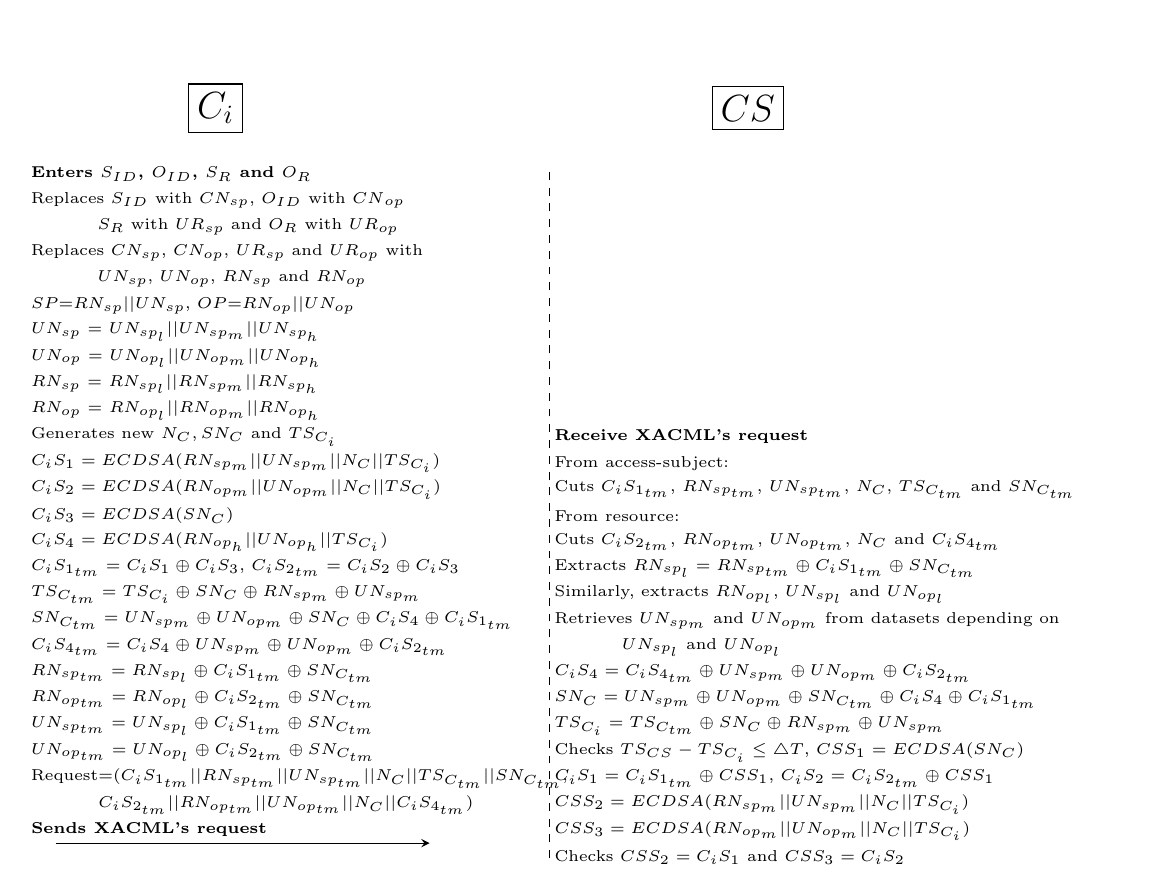
\begin{tikzpicture}
\scalebox{0.95}{
\notsotiny

% to draw vertical dashed line
\draw [dashed] (7.8,2.1) -- (7.8,11.3);

% to write entities
\node [right=2cm] at (25pt,345pt){\Large\textbf{\fbox{$C_i$}}};
\node [right=9cm] at (25pt,345pt){\Large\textbf{\fbox{$CS$}}};
%Client side:
\node [right=-0.1cm] at (25pt,320pt){\textbf{Enters $S_{ID}$, $O_{ID}$, $S_R$ and $O_R$}};
\node [right=-0.1cm] at (25pt,310pt){Replaces $S_{ID}$ with $CN_{sp}$, $O_{ID}$ with ${CN}_{op}$};
\node [right=0.79cm] at (25pt,300pt){$S_R$ with $UR_{sp}$ and $O_R$ with $UR_{op}$};
\node [right=-0.1cm] at (25pt,290pt) {Replaces $CN_{sp}$, $CN_{op}$, $UR_{sp}$ and $UR_{op}$ with};
\node [right=0.79cm] at (25pt,280pt) {$UN_{sp}$, $UN_{op}$, $RN_{sp}$ and $RN_{op}$};
\node [right=-0.1cm] at (25pt,270pt){$SP$=$RN_{sp}||UN_{sp}$, $OP$=$RN_{op}||UN_{op}$};
\node [right=-0.1cm] at (25pt,260pt) {$UN_{sp}$ = $UN_{sp_{l}}||UN_{sp_{m}}||UN_{sp_{h}}$};
\node [right=-0.1cm] at (25pt,250pt) {$UN_{op}$ = $UN_{op_{l}}||UN_{op_{m}}||UN_{op_{h}}$};
\node [right=-0.1cm] at (25pt,240pt) {$RN_{sp}$ = $RN_{sp_{l}}||RN_{sp_{m}}||RN_{sp_{h}}$};
\node [right=-0.1cm] at (25pt,230pt) {$RN_{op}$ = $RN_{op_{l}}||RN_{op_{m}}||RN_{op_{h}}$};
\node [right=-0.1cm] at (25pt,220pt) {Generates new $N_{C}, SN_{C}$ and $TS_{C_i}$};
\node [right=-0.1cm] at (25pt,210pt) {$C_iS_1=ECDSA(RN_{sp_{m}}||UN_{sp_{m}}||N_{C}||TS_{C_i})$};
\node [right=-0.1cm] at (25pt,200pt) {$C_iS_2=ECDSA(RN_{op_m}||UN_{op_m}||N_{C}||TS_{C_i})$};
\node [right=-0.1cm] at (25pt,190pt) {$C_iS_3=ECDSA(SN_{C})$};
\node [right=-0.1cm] at (25pt,180pt) {$C_iS_4=ECDSA(RN_{op_h}||UN_{op_h}||TS_{C_i})$};
\node [right=-0.1cm] at (25pt,170pt) {$C_iS_{1_{tm}}=C_iS_1\oplus C_iS_3$, $C_iS_{2_{tm}}=C_iS_2\oplus C_iS_3$};
\node [right=-0.1cm] at (25pt,160pt) {$TS_{C_{tm}}=TS_{C_i}\oplus SN_{C}\oplus RN_{sp_m}\oplus UN_{sp_m}$};
\node [right=-0.1cm] at (25pt,150pt) {$SN_{C_{tm}}=UN_{sp_m}\oplus UN_{op_m}\oplus SN_C\oplus C_iS_4\oplus C_iS_{1_{tm}}$};
\node [right=-0.1cm] at (25pt,140pt) {$C_iS_{4_{tm}}=C_iS_4\oplus UN_{sp_m}\oplus UN_{op_m}\oplus C_iS_{2_{tm}}$};
\node [right=-0.1cm] at (25pt,130pt) {$RN_{sp_{tm}}=RN_{sp_{l}}\oplus C_iS_{1_{tm}}\oplus SN_{C_{tm}}$};
\node [right=-0.1cm] at (25pt,120pt) {$RN_{op_{tm}}=RN_{op_{l}}\oplus C_iS_{2_{tm}}\oplus SN_{C_{tm}}$};
\node [right=-0.1cm] at (25pt,110pt) {$UN_{sp_{tm}}=UN_{sp_{l}}\oplus C_iS_{1_{tm}}\oplus SN_{C_{tm}}$};
\node [right=-0.1cm] at (25pt,100pt) {$UN_{op_{tm}}=UN_{op_{l}}\oplus C_iS_{2_{tm}}\oplus SN_{C_{tm}}$};
\node [right=-0.1cm] at (25pt,90pt) {Request=($C_iS_{1_{tm}}||RN_{sp_{tm}}||UN_{sp_{tm}}||N_{C}||TS_{C_{tm}}||SN_{C_{tm}}$,};
\node [right=0.8cm] at (25pt,80pt) {$C_iS_{2_{tm}}||RN_{op_{tm}}||UN_{op_{tm}}||N_{C}||C_iS_{4_{tm}}$)};
% to draw arrow with text
\draw [->,>=stealth] (1.2,2.3) -- (6.2,2.3) node[above,pos=0.25] {\textbf{Sends XACML's request}};

%Central Server side:
\node [right=6.9cm] at (25pt,220pt) {\textbf{Receive XACML's request}};
\node [right=6.9cm] at (25pt,210pt) {From access-subject:};
\node [right=6.9cm] at (25pt,200pt) {Cuts $C_iS_{1_{tm}}$, $RN_{sp_{tm}}$, $UN_{sp_{tm}}$, $N_{C}$, $TS_{C_{tm}}$ and $SN_{C_{tm}}$};
\node [right=6.9cm] at (25pt,190pt) {From resource:};
\node [right=6.9cm] at (25pt,180pt) {Cuts $C_iS_{2_{tm}}$, $RN_{op_{tm}}$, $UN_{op_{tm}}$, $N_{C}$  and $C_iS_{4_{tm}}$};
\node [right=6.9cm] at (25pt,170pt) {Extracts $RN_{sp_l}=RN_{sp_{tm}}\oplus C_iS_{1_{tm}}\oplus SN_{C_{tm}}$};
\node [right=6.9cm] at (25pt,160pt) {Similarly, extracts $RN_{op_l}$, $UN_{sp_l}$ and $UN_{op_l}$ };
\node [right=6.9cm] at (25pt,150pt) {Retrieves $UN_{sp_{m}}$ and $UN_{op_{m}}$ from datasets depending on};
\node [right=7.8cm] at (25pt,140pt) {$UN_{sp_l}$ and $UN_{op_l}$};
\node [right=6.9cm] at (25pt,130pt) {$C_iS_4=C_iS_{4_{tm}}\oplus UN_{sp_m}\oplus UN_{op_m}\oplus C_iS_{2_{tm}}$};
\node [right=6.9cm] at (25pt,120pt) {$SN_C=UN_{sp_m}\oplus UN_{op_m}\oplus SN_{C_{tm}}\oplus C_iS_4\oplus C_iS_{1_{tm}}$};
\node [right=6.9cm] at (25pt,110pt) {$TS_{C_i}=TS_{C_{tm}}\oplus SN_C\oplus RN_{sp_m}\oplus UN_{sp_m}$};
\node [right=6.9cm] at (25pt,100pt) {Checks $TS_{CS}-TS_{C_i}\leq \triangle T$, $CSS_1=ECDSA(SN_C)$};
\node [right=6.9cm] at (25pt,90pt) {$C_iS_1=C_iS_{1_{tm}}\oplus CSS_1$, $C_iS_2=C_iS_{2_{tm}}\oplus CSS_1$};
\node [right=6.9cm] at (25pt,80pt) {$CSS_2=ECDSA(RN_{sp_{m}}||UN_{sp_{m}}||N_{C}||TS_{C_i})$};
\node [right=6.9cm] at (25pt,70pt) {$CSS_3=ECDSA(RN_{op_m}||UN_{op_m}||N_{C}||TS_{C_i})$};
\node [right=6.9cm] at (25pt,60pt) {Checks $CSS_2=C_iS_1$ and $CSS_3=C_iS_2$};
}
\end{tikzpicture}
	\caption{Protocol of PAX model between $C_i$ and $CS$.}
	\label{fig:pax_ci_cs}
\end{figure*}
\item Second protocol as shown in Figure~\ref{fig:pax_cs_as}:
\begin{itemize}
\item $CS$ generates random secret ($SN_{CS}$) and new timestamp ($TS_{CS}$) between $CS$ and $AS$. Then, $CS$ computes the secret signature ($CSS_4$) to protect $SN_{CS}$. Also, $CS$ hides $C_i$'s parameters such as $N_C$ and $TS_{C_i}$ to use them with validation operations in $AS$ and  $DS$. In addition, all Sigs (such as $CSS_{2_{tm}}$) and PP (such as $N_{CS}$ and $TS_{CS_{tm}}$) are anonymously hidden by $CS$. At this point, $CS$ sends XACML's request to $AS$.
\item $AS$ receives the request, cuts Sigs and PP. After that, $AS$ extracts original parameters (such as $C_iS_4$ and $TS_{CS}$) and checks timestamp. $AS$ computes $ASS_1$ (to extract $CSS_2$ and $CSS_3$) and computes $ASS_2$ and $ASS_3$ (to check $ASS_2$=$CSS_2$ and $ASS_3$=$CSS_3$). $AS$ retrieves $RN_{op_h}$ and $UN_{op_h}$ from dataset (depending on $RN_{op_m}$ and $UN_{op_m}$) and computes $ASS_4$ to ensure $C_i$ request is legitimate after checks $ASS_4=C_iS_4$. $AS$ uses the parts of external pseudonyms to specify $UR_{sp}$, $UR_{op}$, $CN_{sp}$ and $CN_{sp}$. $AS$ retrieves Sigs of $SP$ and $OP$ ($S_{sp}$ and $S_{op}$) depending on the internal $SP$ and $OP$. $AS$ uses PDP1 engine to evaluate XACML's request after adding $S_{sp}$ and $S_{op}$ to that request. $AS$ specifies user's policy in PAP and checks user's attributes in PIP. PDP1 applies policy to get a decision (permit, deny, not applicable and indeterminate). If decision="permit", $AS$ uses $UR_{sp}$ to specify user's role (direct/indirect). If $UR_{sp}$=direct, $AS$ sends the data retrieval request by PRP to $DS$; if $UR_{sp}$=indirect, $AS$ sends the Shamir request that contain at least 2 $SS_s$ to insure legitimate indirect users. Otherwise $AS$ sends reject response to $C_i$ by $CS$.
\end{itemize}
% Authorisation for direct user (CS to AS)
\begin{figure*}[ht]
\centering
\scriptsize
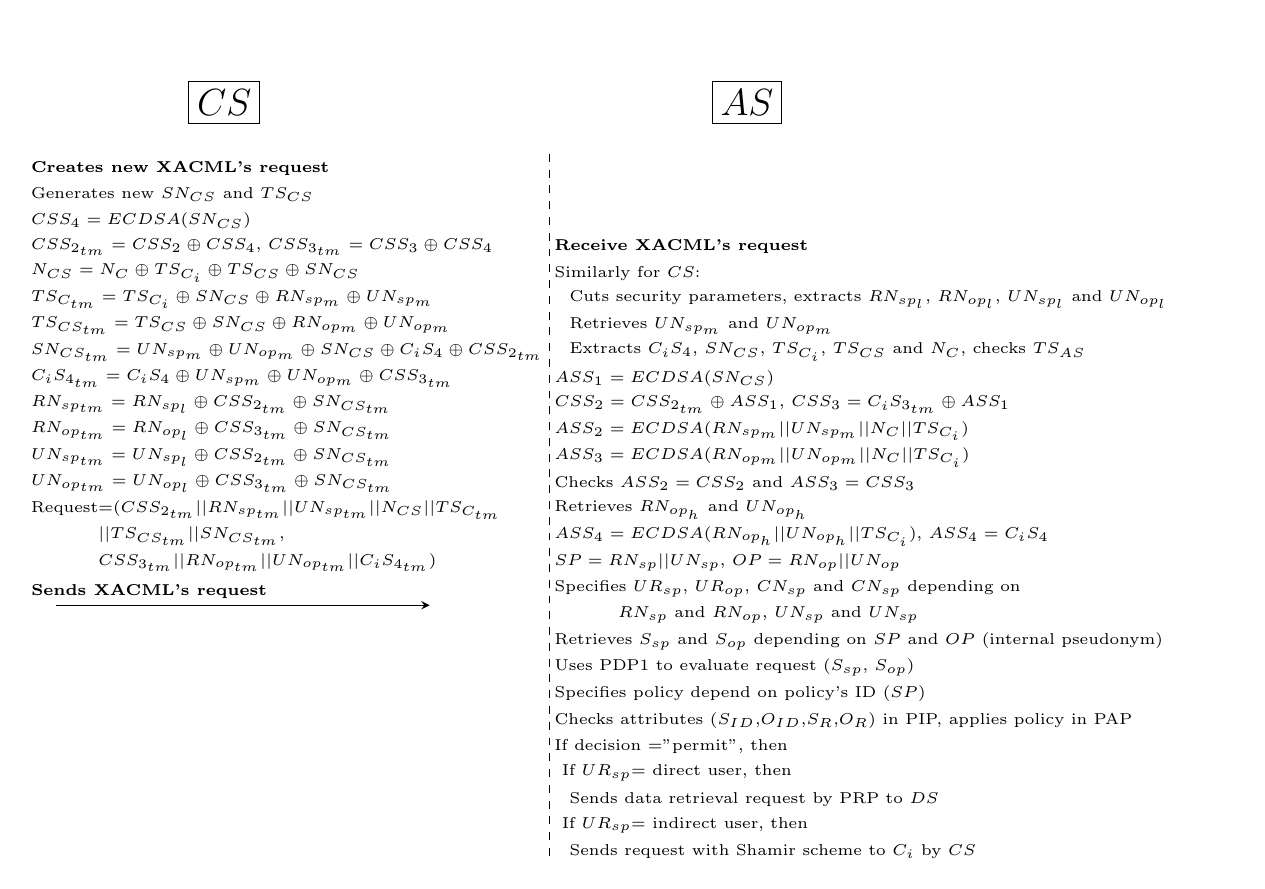
\begin{tikzpicture}
\scalebox{0.95}{
\notsotiny

% to draw vertical dashed line
\draw [dashed] (7.8,1.35) -- (7.8,10.8);

% to write entities
\node [right=2cm] at (25pt,325pt){\Large\textbf{\fbox{$CS$}}};
\node [right=9cm] at (25pt,325pt){\Large\textbf{\fbox{$AS$}}};
%Client side:
\node [right=-0.1cm] at (25pt,300pt){\textbf{Creates new XACML's request}};
\node [right=-0.1cm] at (25pt,290pt) {Generates new $SN_{CS}$ and $TS_{CS}$};
\node [right=-0.1cm] at (25pt,280pt) {$CSS_4=ECDSA(SN_{CS})$};
\node [right=-0.1cm] at (25pt,270pt) {$CSS_{2_{tm}}=CSS_2\oplus CSS_4$, $CSS_{3_{tm}}=CSS_3\oplus CSS_4$};
\node [right=-0.1cm] at (25pt,260pt) {$N_{CS}=N_{C}\oplus TS_{C_i}\oplus TS_{CS}\oplus SN_{CS}$};
\node [right=-0.1cm] at (25pt,250pt) {$TS_{C_{tm}}=TS_{C_i}\oplus SN_{CS}\oplus RN_{sp_m}\oplus UN_{sp_m}$};
\node [right=-0.1cm] at (25pt,240pt) {$TS_{CS_{tm}}=TS_{CS}\oplus SN_{CS}\oplus RN_{op_m}\oplus UN_{op_m}$};
\node [right=-0.1cm] at (25pt,230pt) {$SN_{CS_{tm}}=UN_{sp_m}\oplus UN_{op_m}\oplus SN_{CS}\oplus C_iS_4\oplus CSS_{2_{tm}}$};
\node [right=-0.1cm] at (25pt,220pt) {$C_iS_{4_{tm}}=C_iS_4\oplus UN_{sp_m}\oplus UN_{op_m}\oplus CSS_{3_{tm}}$};
\node [right=-0.1cm] at (25pt,210pt) {$RN_{sp_{tm}}=RN_{sp_{l}}\oplus CSS_{2_{tm}}\oplus SN_{CS_{tm}}$};
\node [right=-0.1cm] at (25pt,200pt) {$RN_{op_{tm}}=RN_{op_{l}}\oplus CSS_{3_{tm}}\oplus SN_{CS_{tm}}$};
\node [right=-0.1cm] at (25pt,190pt) {$UN_{sp_{tm}}=UN_{sp_{l}}\oplus CSS_{2_{tm}}\oplus SN_{CS_{tm}}$};
\node [right=-0.1cm] at (25pt,180pt) {$UN_{op_{tm}}=UN_{op_{l}}\oplus CSS_{3_{tm}}\oplus SN_{CS_{tm}}$};
\node [right=-0.1cm] at (25pt,170pt) {Request=($CSS_{2_{tm}}||RN_{sp_{tm}}||UN_{sp_{tm}}||N_{CS}||TS_{C_{tm}}$};
\node [right=0.8cm] at (25pt,160pt) {$||TS_{CS_{tm}}||SN_{CS_{tm}}$,};
\node [right=0.8cm] at (25pt,150pt) {$CSS_{3_{tm}}||RN_{op_{tm}}||UN_{op_{tm}}||C_iS_{4_{tm}}$)};
% to draw arrow with text
\draw [->,>=stealth] (1.2,4.7) -- (6.2,4.7) node[above,pos=0.25] {\textbf{Sends XACML's request}};

%Attributes Server side:
\node [right=6.9cm] at (25pt,270pt){\textbf{Receive XACML's request}};
\node [right=6.9cm] at (25pt,260pt){Similarly for $CS$:};
    \node [right=7.1cm] at (25pt,250pt){Cuts security parameters, extracts $RN_{sp_l}$, $RN_{op_l}$, $UN_{sp_l}$ and $UN_{op_l}$ };
    \node [right=7.1cm] at (25pt,240pt){Retrieves $UN_{sp_m}$ and $UN_{op_m}$};
    \node [right=7.1cm] at (25pt,230pt) {Extracts  $C_iS_4$, $SN_{CS}$, $TS_{C_i}$, $TS_{CS}$ and $N_{C}$, checks $TS_{AS}$};
\node [right=6.9cm] at (25pt,220pt) {$ASS_1=ECDSA(SN_{CS})$};
\node [right=6.9cm] at (25pt,210pt) {$CSS_2=CSS_{2_{tm}}\oplus ASS_1$, $CSS_3=C_iS_{3_{tm}}\oplus ASS_1$};
\node [right=6.9cm] at (25pt,200pt) {$ASS_2=ECDSA(RN_{sp_{m}}||UN_{sp_{m}}||N_{C}||TS_{C_i})$};
\node [right=6.9cm] at (25pt,190pt) {$ASS_3=ECDSA(RN_{op_m}||UN_{op_m}||N_{C}||TS_{C_i})$};
\node [right=6.9cm] at (25pt,180pt) {Checks $ASS_2=CSS_2$ and $ASS_3=CSS_3$};
\node [right=6.9cm] at (25pt,170pt){Retrieves $RN_{op_h}$ and $UN_{op_h}$};
\node [right=6.9cm] at (25pt,160pt) {$ASS_4=ECDSA(RN_{op_h}||UN_{op_h}||TS_{C_i})$, $ASS_4=C_iS_4$};
\node [right=6.9cm] at (25pt,150pt) {$SP=RN_{sp}||UN_{sp}$, $OP=RN_{op}||UN_{op}$};

\node [right=6.9cm] at (25pt,140pt){Specifies $UR_{sp}$, $UR_{op}$, $CN_{sp}$ and $CN_{sp}$  depending on};
\node [right=7.75cm] at (25pt,130pt){$RN_{sp}$ and $RN_{op}$, $UN_{sp}$ and $UN_{sp}$};

\node [right=6.9cm] at (25pt,120pt) {Retrieves $S_{sp}$ and $S_{op}$ depending on $SP$ and $OP$ (internal pseudonym) };
\node [right=6.9cm] at (25pt,110pt) {Uses PDP1 to evaluate request ($S_{sp}$, $S_{op}$)};
\node [right=6.9cm] at (25pt,100pt) {Specifies policy depend on policy's ID ($SP$)};
\node [right=6.9cm] at (25pt,90pt) {Checks attributes ($S_{ID}$,$O_{ID}$,$S_R$,$O_R$) in PIP, applies policy in PAP};
\node [right=6.9cm] at (25pt,80pt){If decision ="permit", then };
  \node [right=7cm] at (25pt,70pt) {If $UR_{sp}$= direct user, then};
    \node [right=7.1cm] at (25pt,60pt){Sends data retrieval request by PRP to $DS$};
  \node [right=7cm] at (25pt,50pt) {If $UR_{sp}$= indirect user, then};
    \node [right=7.1cm] at (25pt,40pt){Sends request with Shamir scheme to $C_i$ by $CS$};
}
\end{tikzpicture}
	\caption{Protocol of PAX model between $CS$ and $AS$.}
	\label{fig:pax_cs_as}
\end{figure*}
\item  Third protocol as shown in Figure~\ref{fig:pax_as_ds}:
\begin{itemize}
\item Similarly, $AS$ generates random secret ($SN_{AS}$) and timestamp ($TS_{AS}$) between $AS$ and $DS$. $AS$ computes $ASS_{5}$ to protect secret ($SN_{AS}$) between $AS$ and $DS$. Additionally, $AS$ computes $ASS_{6}$ to ensure legitimate PP ($RN_{op_m}$ and $UN_{op_m}$) in $DS$. All Sigs (such as $ASS_{6_{tm}}$) and PP (such as $TS_{AS_{tm}}$ and $SN_{AS_{tm}}$) are anonymously hidden by $AS$. Then, $AS$ sends XACML's request to $DS$.
\item $DS$ receives the request, cuts Sigs and PP. After that, $DS$ extracts original parameters (such as $C_iS_4$ and $SN_{AS}$) and checks timestamp. $DS$ computes $DSS_1$ (to extract $ASS_6$) and retrieves $RN_{op_h}$ and $RN_{op_m}$ depending on $RN_{op_l}$. Then, $DS$ computes $DSS_2$ and $DSS_3$ to check $DSS_2=ASS_6$ and $DSS_3=C_iS_4$. If $AS$'s parameters validated in $DS$ correctly, $DS$ computes timestamp ($TS_{DS}$) and signs patient's data ($DSS_4$). All Sigs (such as $DSS_{4_{tm}}$) and PP (such as $TS_{DS_{tm}}$) are anonymously hidden by $DS$. At this point, $DS$ sends the response to $AS$.
\item $AS$ receives the response, extracts PP (such as $TS_{DS}$) and checks timestamp. $AS$ tests the Sigs checking (such as $ASS_6=DSS_2$). Then, $AS$ computes data signature ($ASS_7$) to check data integrity by $ASS_7=DSS_4$.
\end{itemize}
% Authorisation for direct user (AS to DS)
\begin{figure*}[ht]
\centering
\scriptsize
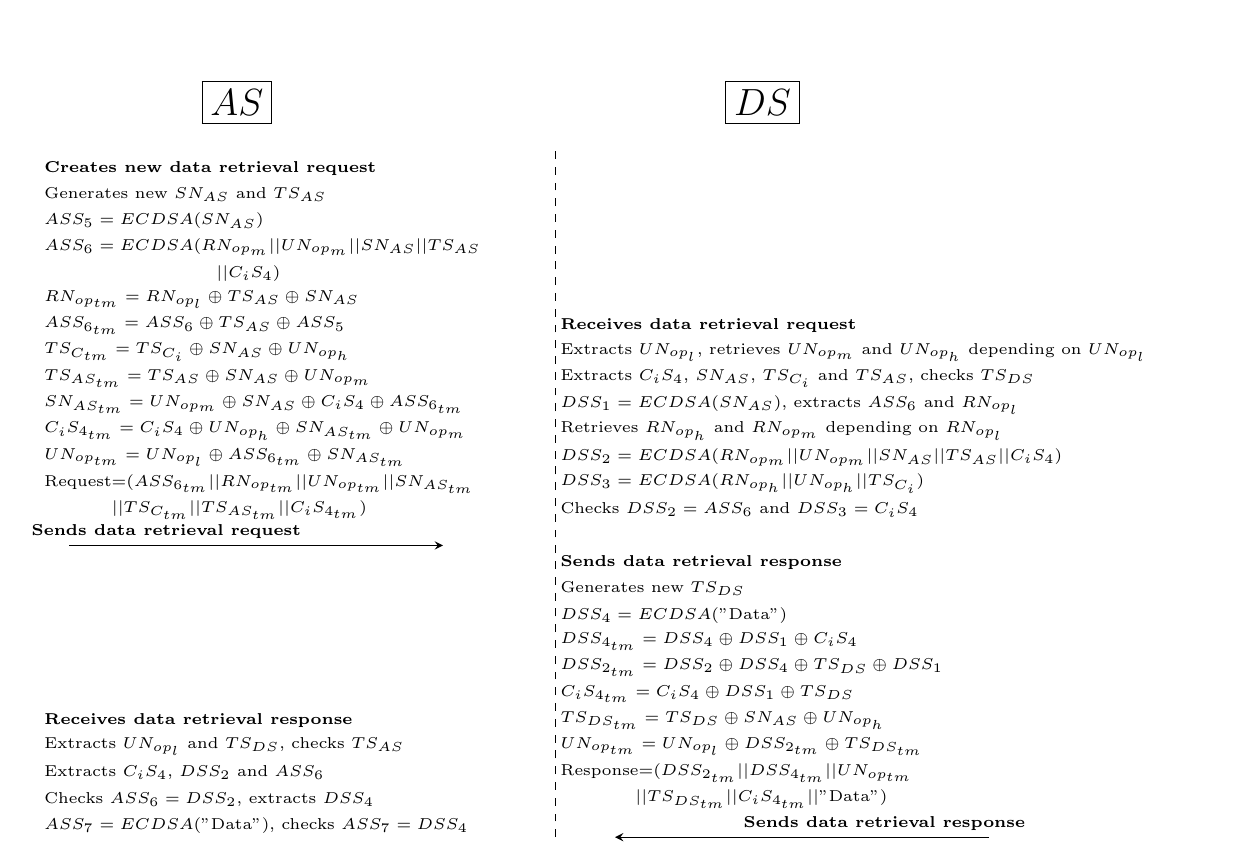
\begin{tikzpicture}
\scalebox{0.95}{
\notsotiny

% to draw vertical dashed line
\draw [dashed] (7.7,1.6) -- (7.7,10.8);

% to write entities
\node [right=2cm] at (25pt,325pt){\Large\textbf{\fbox{$AS$}}};
\node [right=9cm] at (25pt,325pt){\Large\textbf{\fbox{$DS$}}};
%Attributes Server side:
\node [right=-0.1cm] at (25pt,300pt){\textbf{Creates new data retrieval request}};
\node [right=-0.1cm] at (25pt,290pt) {Generates new  $SN_{AS}$ and $TS_{AS}$};
\node [right=-0.1cm] at (25pt,280pt) {$ASS_5=ECDSA(SN_{AS})$};
\node [right=-0.1cm] at (25pt,270pt) {$ASS_6=ECDSA(RN_{op_m}||UN_{op_m}||SN_{AS}||TS_{AS}$};
\node [right=2.2cm] at (25pt,260pt) {$||C_iS_4)$};
\node [right=-0.1cm] at (25pt,250pt) {$RN_{op_{tm}}=RN_{op_l}\oplus TS_{AS}\oplus SN_{AS}$};
\node [right=-0.1cm] at (25pt,240pt) {$ASS_{6_{tm}}=ASS_6\oplus TS_{AS}\oplus ASS_5$};
\node [right=-0.1cm] at (25pt,230pt) {$TS_{C_{tm}}=TS_{C_i}\oplus SN_{AS}\oplus UN_{op_h}$};
\node [right=-0.1cm] at (25pt,220pt) {$TS_{AS_{tm}}=TS_{AS}\oplus SN_{AS}\oplus UN_{op_m}$};
\node [right=-0.1cm] at (25pt,210pt) {$SN_{AS_{tm}}=UN_{op_m}\oplus SN_{AS}\oplus C_iS_4\oplus ASS_{6_{tm}}$};
\node [right=-0.1cm] at (25pt,200pt) {$C_iS_{4_{tm}}=C_iS_4\oplus UN_{op_h}\oplus SN_{AS_{tm}}\oplus UN_{op_m}$};
\node [right=-0.1cm] at (25pt,190pt) {$UN_{op_{tm}}=UN_{op_{l}}\oplus ASS_{6_{tm}}\oplus SN_{AS_{tm}}$};
\node [right=-0.1cm] at (25pt,180pt) {Request=($ASS_{6_{tm}}||RN_{op_{tm}}||UN_{op_{tm}}||SN_{AS_{tm}}$};
\node [right=0.8cm] at (25pt,170pt) {$||TS_{C_{tm}}||TS_{AS_{tm}}||C_iS_{4_{tm}}$)};
% to draw arrow with text
\draw [->,>=stealth] (1.2,5.5) -- (6.2,5.5) node[above,pos=0.26] {\textbf{Sends data retrieval request}};

%Data Server side:
\node [right=6.8cm] at (25pt,240pt){\textbf{Receives data retrieval request}};
\node [right=6.8cm] at (25pt,230pt){Extracts $UN_{op_l}$, retrieves $UN_{op_m}$ and $UN_{op_h}$ depending on $UN_{op_l}$};
\node [right=6.8cm] at (25pt,220pt){ Extracts $C_iS_4$, $SN_{AS}$, $TS_{C_i}$ and $TS_{AS}$, checks $TS_{DS}$};
\node [right=6.8cm] at (25pt,210pt){$DSS_1=ECDSA(SN_{AS})$, extracts $ASS_6$ and $RN_{op_l}$};
\node [right=6.8cm] at (25pt,200pt){Retrieves $RN_{op_h}$ and $RN_{op_m}$  depending on  $RN_{op_l}$};
\node [right=6.8cm] at (25pt,190pt){$DSS_2=ECDSA(RN_{op_{m}}||UN_{op_{m}}||SN_{AS}||TS_{AS}||C_iS_4)$};
\node [right=6.8cm] at (25pt,180pt) {$DSS_3=ECDSA(RN_{op_h}||UN_{op_h}||TS_{C_i})$};
\node [right=6.8cm] at (25pt,170pt) {Checks $DSS_2=ASS_6$ and $DSS_3=C_iS_4$};

\node [right=6.8cm] at (25pt,150pt){\textbf{Sends data retrieval response}};
\node [right=6.8cm] at (25pt,140pt) {Generates new  $TS_{DS}$};
\node [right=6.8cm] at (25pt,130pt) {$DSS_4=ECDSA($"Data"$)$};
\node [right=6.8cm] at (25pt,120pt) {$DSS_{4_{tm}}=DSS_4\oplus DSS_1\oplus C_iS_4$};
\node [right=6.8cm] at (25pt,110pt) {$DSS_{2_{tm}}=DSS_2\oplus DSS_4\oplus TS_{DS}\oplus DSS_1$};
\node [right=6.8cm] at (25pt,100pt) { $C_iS_{4_{tm}}=C_iS_4\oplus DSS_1\oplus TS_{DS}$};
\node [right=6.8cm] at (25pt,90pt) {$TS_{DS_{tm}}=TS_{DS}\oplus SN_{AS}\oplus UN_{op_h}$};
\node [right=6.8cm] at (25pt,80pt) {$UN_{op_{tm}}=UN_{op_l}\oplus DSS_{2_{tm}}\oplus TS_{DS_{tm}}$};
\node [right=6.8cm] at (25pt,70pt) {Response=($DSS_{2_{tm}}||DSS_{4_{tm}}||UN_{op_{tm}}$};
\node [right=7.8cm] at (25pt,60pt) {$||TS_{DS_{tm}}||C_iS_{4_{tm}}||$"Data")};
% to draw arrow with text
\draw [->,>=stealth] (13.5,1.6) -- (8.5,1.6) node[above,pos=0.28] {\textbf{Sends data retrieval response}};

% Attribute server side
\node [right=-0.1cm] at (25pt,90pt){\textbf{Receives data retrieval response}};
\node [right=-0.1cm] at (25pt,80pt) {Extracts $UN_{op_l}$  and $TS_{DS}$, checks $TS_{AS}$ };
\node [right=-0.1cm] at (25pt,70pt) {Extracts $C_iS_4$, $DSS_2$ and $ASS_6$  };
\node [right=-0.1cm] at (25pt,60pt) {Checks $ASS_6=DSS_2$, extracts $DSS_4$};
\node [right=-0.1cm] at (25pt,50pt) {$ASS_7=ECDSA($"Data"$)$, checks $ASS_7=DSS_4$};
}
\end{tikzpicture}
	\caption{Protocol of PAX model between $AS$ and $DS$.}
	\label{fig:pax_as_ds}
\end{figure*}
\item Fourth protocol as shown in Figure~\ref{fig:pax_as_cs_ci}:
\begin{itemize}
\item $AS$ prepares the response to $CS$ by generating a new timestamp ($TS_{AS}$), hides data signature ($ASS_7$) with $ASS_2$, $ASS_3$, $C_iS_4$ and secret signature ($ASS_1$). $AS$ hides PP and sends the response that contains decision and patient's data to $CS$.
\item $CS$ receives the response and extracts Sigs and PP. $CS$ computes data signature ($DSS_5$) to check data integrity ($CSS_5=ASS_7$). Then, $CS$ checks other Sigs ($CSS_2$, $CSS_3$ and $CSS_4$) with received Sigs ($ASS_2$, $ASS_3$ and $C_iS_4$) to ensure legitimacy of $AS$. $CS$ prepares the response to $C_i$ by generating a new timestamp and hides data signature ($CSS_5$) with $CSS_2$, $CSS_3$, $C_iS_4$ and secret signature ($CSS_1$). $CS$ sends the response to $C_i$.
\item $C_i$ receives the response, extracts PP and checks timestamp. $C_i$ computes data signature ($C_iS_5$) to check data integrity by $C_iS_5=CSS_5$. Then, $C_i$ extracts signatures ($CSS_2$, $CSS_3$, $CSS_1$ and $C_iS_4$) and checks them with original signatures ($C_iS_1$, $C_iS_2$, $C_iS_3$ and $C_iS_4$) respectively. $C_i$ uses $CSS_2$, $CSS_3$ and $CSS_1$ (secret signature between $C_i$ and $CS$) to check legitimacy of $CS$ while uses $C_iS_4$ to check legitimacy of $AS$ and $DS$. If all Sigs are validated, namely, authorised $C_i$ received securely correct data.
\end{itemize}
% Authorisation for direct user (AS_CS_Ci)
\begin{figure*}[t]
\centering
\scriptsize
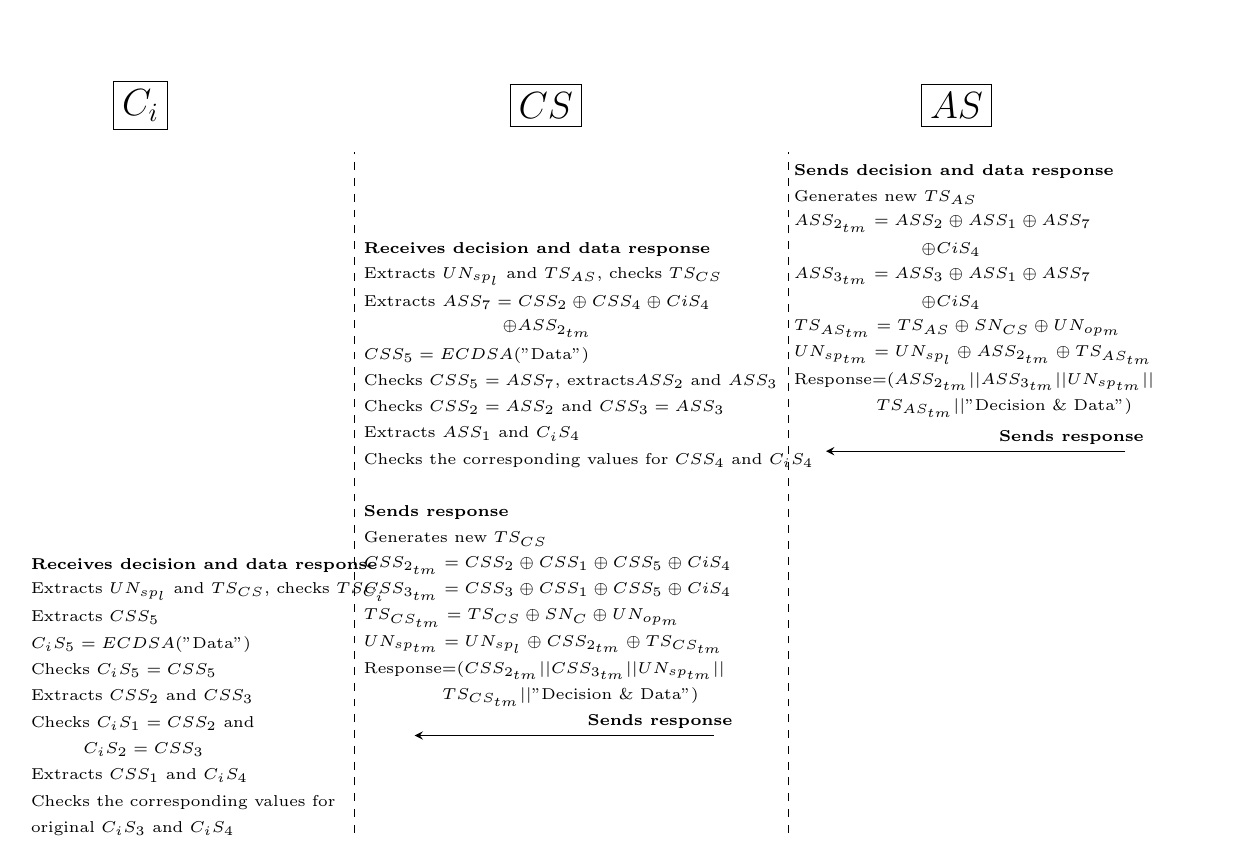
\begin{tikzpicture}
\scalebox{0.95}{ % to reduce font
\notsotiny

% to draw vertical dashed line
\draw [dashed] (5.2,1.7) -- (5.2,10.8);
\draw [dashed] (11.0,1.7) -- (11.0,10.8);

% to write entities
\node [right=1cm] at (25pt,325pt){\Large\textbf{\fbox{$C_i$}}};
\node [right=6.3cm] at (25pt,325pt){\Large\textbf{\fbox{$CS$}}};
\node [right=11.8cm] at (25pt,325pt){\Large\textbf{\fbox{$AS$}}};

%Attributes Server side:
\node [right=10.1cm] at (25pt,300pt){\textbf{Sends decision and data response}};
\node [right=10.1cm] at (25pt,290pt){Generates new $TS_{AS}$};
\node [right=10.1cm] at (25pt,280pt){$ASS_{2_{tm}}=ASS_2\oplus ASS_1\oplus ASS_7$};
\node [right=11.8cm] at (25pt,270pt){$\oplus CiS_4$};
\node [right=10.1cm] at (25pt,260pt){$ASS_{3_{tm}}=ASS_3\oplus ASS_1\oplus ASS_7$};
\node [right=11.8cm] at (25pt,250pt){$\oplus CiS_4$};
\node [right=10.1cm] at (25pt,240pt){$TS_{AS_{tm}}=TS_{AS}\oplus SN_{CS}\oplus UN_{op_m}$};
\node [right=10.1cm] at (25pt,230pt){$UN_{sp_{tm}}=UN_{sp_l}\oplus ASS_{2_{tm}}\oplus TS_{AS_{tm}}$};
\node [right=10.1cm] at (25pt,220pt){Response=($ASS_{2_{tm}}||ASS_{3_{tm}}||UN_{sp_{tm}}||$};
\node [right=11.2cm] at (25pt,210pt){$TS_{AS_{tm}}||$"Decision \& Data")};
% to draw arrow with text
\draw [->,>=stealth] (15.5,6.8) -- (11.5,6.8) node[above,pos=0.18] {\textbf{Sends  response}};

%Central Server side:
\node [right=4.35cm] at (25pt,270pt){\textbf{Receives decision and data response}};
\node [right=4.35cm] at (25pt,260pt){Extracts $UN_{sp_l}$ and $TS_{AS}$, checks $TS_{CS}$};
\node [right=4.35cm] at (25pt,250pt){Extracts $ASS_7=CSS_2\oplus CSS_4\oplus CiS_4$};
\node [right=6.2cm] at (25pt,240pt){$\oplus ASS_{2_{tm}}$};
\node [right=4.35cm] at (25pt,230pt){$CSS_5=ECDSA($"Data")};
\node [right=4.35cm] at (25pt,220pt){Checks $CSS_5=ASS_7$, extracts$ASS_2$ and $ASS_3$};
\node [right=4.35cm] at (25pt,210pt){Checks $CSS_2=ASS_2$ and $CSS_3=ASS_3$};
\node [right=4.35cm] at (25pt,200pt){Extracts $ASS_1$ and $C_iS_4$};
\node [right=4.35cm] at (25pt,190pt){Checks the corresponding values for $CSS_4$ and $C_iS_4$};

\node [right=4.35cm] at (25pt,170pt){\textbf{Sends  response}};
\node [right=4.35cm] at (25pt,160pt){Generates new $TS_{CS}$};
\node [right=4.35cm] at (25pt,150pt){$CSS_{2_{tm}}=CSS_2\oplus CSS_1\oplus CSS_5\oplus CiS_4$};
\node [right=4.35cm] at (25pt,140pt){$CSS_{3_{tm}}=CSS_3\oplus CSS_1\oplus CSS_5\oplus CiS_4$};
\node [right=4.35cm] at (25pt,130pt){$TS_{CS_{tm}}=TS_{CS}\oplus SN_{C}\oplus UN_{op_m}$};
\node [right=4.35cm] at (25pt,120pt){$UN_{sp_{tm}}=UN_{sp_l}\oplus CSS_{2_{tm}}\oplus TS_{CS_{tm}}$};
\node [right=4.35cm] at (25pt,110pt){Response=($CSS_{2_{tm}}||CSS_{3_{tm}}||UN_{sp_{tm}}||$};
\node [right=5.4cm] at (25pt,100pt){$TS_{CS_{tm}}||$"Decision \& Data")};
% to draw arrow with text
\draw [->,>=stealth] (10,3) -- (6,3) node[above,pos=0.18] {\textbf{Sends response}};

% Clienti
\node [right=-0.1cm] at (25pt,150pt){\textbf{Receives decision and data response}};
\node [right=-0.1cm] at (25pt,140pt){Extracts $UN_{sp_l}$ and $TS_{CS}$, checks $TS_{C_i}$};
\node [right=-0.1cm] at (25pt,130pt){Extracts $CSS_5$};
\node [right=-0.1cm] at (25pt,120pt){$C_iS_5=ECDSA($"Data")};
\node [right=-0.1cm] at (25pt,110pt){Checks $C_iS_5=CSS_5$};
\node [right=-0.1cm] at (25pt,100pt){Extracts $CSS_2$ and $CSS_3$};
\node [right=-0.1cm] at (25pt,90pt){Checks $C_iS_1=CSS_2$ and};
\node [right=0.6cm] at (25pt,80pt){$C_iS_2=CSS_3$};
\node [right=-0.1cm] at (25pt,70pt){Extracts $CSS_1$ and $C_iS_4$ };
\node [right=-0.1cm] at (25pt,60pt){Checks the corresponding values for};
\node [right=-0.1cm] at (25pt,50pt){original $C_iS_3$ and $C_iS_4$};
}
\end{tikzpicture}
	\caption{Protocol of PAX model between $AS$, $CS$ and $C_i$.}
	\label{fig:pax_as_cs_ci}
\end{figure*}
\end{enumerate}
\end{itemize}
\item \textbf{Authorisation protocols for indirect subjects and objects}\\
Authorisation of indirect users is an important process to secure sensitive patients' data 
in the EHR stored in $DS$. PAX offers additional procedures to prevent the abuse of indirect 
user privileges.
\begin{itemize}[topsep=0pt,itemsep=-1ex,partopsep=1ex,parsep=1ex]
\item \textbf{Prerequisite procedures}\\
There are a set of steps that must be performed before the authorisation protocols are applied.
\begin{enumerate}
\item Steps from 1 to 3 are similar to those for direct users.
\item The Shamir scheme is used to generate the $SS_s$ from $MS$ for the number of users, each $C_i$ has unique $SS$ same length as $MS$, and authorised with two policies for each indirect user on $AS$. The policy evaluation process is also done with two, PDP1 and PDP2, evaluation engines. The use of two evaluation engines is very important in separating direct and indirect users and increasing security in the privacy of medical records.
\item The PAX authorisation system identifies certain medical records (the patients' history at a given time such as a year or more ago) for indirect users who can access them, as shown in Figure~\ref{fig:patientsdata} (researcher case).
\end{enumerate}
\item \textbf{Authorisation protocols}\\
The following protocols detail how the indirect user obtains medical records in PAX. Figure~\ref{fig:indirectuser} illustrates generally the authorisation of indirect users, while Figures~\ref{fig:pax_ci_cs}, \ref{fig:pax_cs_as},  \ref{fig:pax_indirectuser}, \ref{fig:pax_as_ds}, and \ref{fig:pax_as_cs_ci} show the authorisation protocols of indirect users in PAX.
\begin{figure*}[t!]
\centering
  \includegraphics[width=14cm,height=7cm]{indirectuser.png}
	\caption{Authorisation of indirect users.}
	\label{fig:indirectuser}
\end{figure*}
\begin{enumerate}
\item The steps of the first and second protocols are similar to the ones of the direct users authorisation.
\item Third protocol as shown in Figure~\ref{fig:pax_indirectuser}:
\begin{itemize}
\item $AS$ computed $MS$ previously by signing all users' signatures. Then, $AS$ computes Shamir scheme to generate $SS_s$ with the same number of users (each $C_i$ has one unique $SS$). In PAX, $C_i$ needs at least 3 $SS_s$ to generate original $MS$. In this protocol, $AS$ generates a new timestamp and retrieves at least 2 $SS_s$. After that, $AS$ hides $SS_s$ with $ASS_2$, $C_iS_4$, $S_{sp}$ and secret signature ($ASS_1$) as well as parameters (such as $TS_{AS_{tm}}$ and $UN_{sp_{tm}}$) are anonymously hidden. At this point, $AS$ sends request to $CS$.
\item $CS$ receives the request, extracts PP and checks timestamp. Then, $CS$ removes the secret signature ($CSS_4$) and adds the secret signature ($CSS_1$) in $CSS_{2_{tm}}$. $CS$ generates a new timestamp ($TS_{CS}$), hides PP and sends the request to $C_i$.
\item $C_i$ receives Shamir's request, extracts PP and checks timestamp. Then, $C_i$ computes $C_iS_6$ to extract $SS_s$ and retrieves his $SS$. At the moment, $C_i$ can generate $MS$ from Shamir ($C_i$'s $SS$||$SS_s$), hides $MS$ with $C_iS_6$ and $C_iS_3$, generates timestamp and hides PP. At this point, $C_i$ sends the response to $CS$.
\item $CS$ receives the response, extracts PP and checks timestamp. Also, $CS$ removes $CSS_1$ and adds $CSS_4$ in $C_iS_{6_{tm}}$. $CS$ generates a new timestamp, hides PP and sends the response to $AS$.
\item $AS$ receives Shamir response, extracts PP and checks timestamp. Then, $AS$ extracts the received $MS$ and checks it with the saved original $MS$. After that, $AS$ retrieves $C_i$'s $SS$ depending on $S_{sp}$($UR_{sp}||CN_{sp}$) and assigns the request ($SS$,$S_{op}$) to PDP2 . $AS$ specifies policy depending on policy's ID (Shamir||$SP$), checks attributes in PIP and PDP2 applies policy in PAP to produce the decision. If the decision is "permit", $AS$ creates a data retrieval request by PRP to DS; otherwise $AS$ sends reject response to $C_i$ by $CS$.
\end{itemize}
% Authorisation for indirect user (Shamir Scheme)
\begin{figure*}[ht]
\centering
\scriptsize
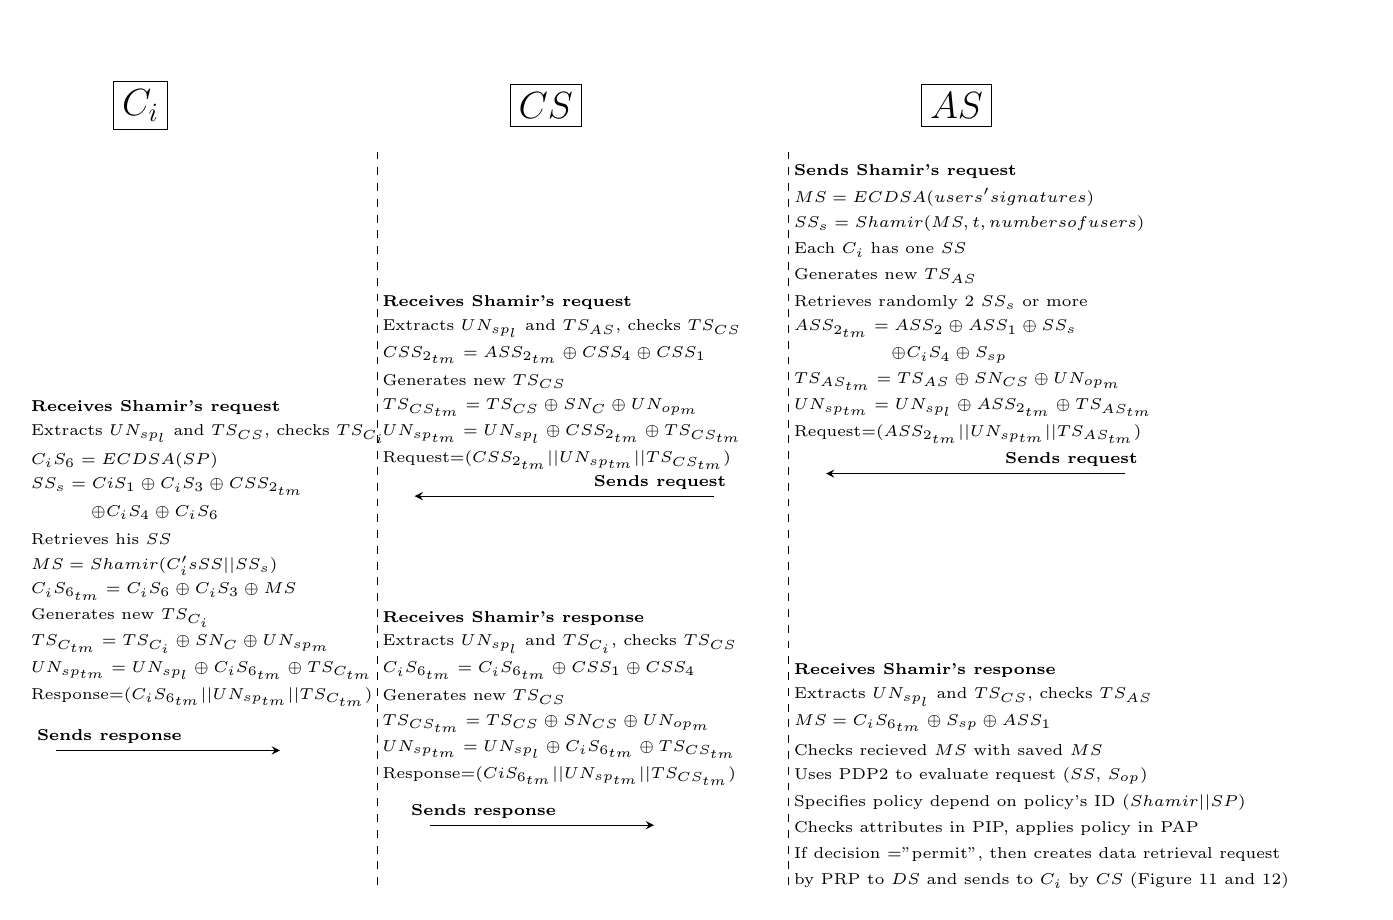
\begin{tikzpicture}
\scalebox{0.95}{ % to reduce font
\notsotiny

% to draw vertical dashed line
\draw [dashed] (5.5,1) -- (5.5,10.8);
\draw [dashed] (11.0,1) -- (11.0,10.8);

% to write entities
\node [right=1cm] at (25pt,325pt){\Large\textbf{\fbox{$C_i$}}};
\node [right=6.3cm] at (25pt,325pt){\Large\textbf{\fbox{$CS$}}};
\node [right=11.8cm] at (25pt,325pt){\Large\textbf{\fbox{$AS$}}};

%Attributes Server side:
\node [right=10.1cm] at (25pt,300pt){\textbf{Sends Shamir's request}};
\node [right=10.1cm] at (25pt,290pt){$MS=ECDSA(users' signatures)$};
\node [right=10.1cm] at (25pt,280pt){$SS_s=Shamir(MS,t,numbers of users)$};
\node [right=10.1cm] at (25pt,270pt){Each $C_i$ has one $SS$};
\node [right=10.1cm] at (25pt,260pt){Generates new $TS_{AS}$};
\node [right=10.1cm] at (25pt,250pt){Retrieves randomly 2 $SS_s$ or more};
\node [right=10.1cm] at (25pt,240pt){$ASS_{2_{tm}}=ASS_2\oplus ASS_1\oplus SS_s$};
\node [right=11.4cm] at (25pt,230pt){$\oplus C_iS_4\oplus S_{sp}$};
\node [right=10.1cm] at (25pt,220pt){$TS_{AS_{tm}}=TS_{AS}\oplus SN_{CS}\oplus UN_{op_m}$};
\node [right=10.1cm] at (25pt,210pt){$UN_{sp_{tm}}=UN_{sp_l}\oplus ASS_{2_{tm}}\oplus TS_{AS_{tm}}$};
\node [right=10.1cm] at (25pt,200pt){Request=($ASS_{2_{tm}}||UN_{sp_{tm}}||TS_{AS_{tm}}$)};
% to draw arrow with text
\draw [->,>=stealth] (15.5,6.5) -- (11.5,6.5) node[above,pos=0.18] {\textbf{Sends request}};

\node [right=10.1cm] at (25pt,110pt){\textbf{Receives Shamir's response}};
\node [right=10.1cm] at (25pt,100pt){Extracts $UN_{sp_l}$ and $TS_{CS}$, checks $TS_{AS}$};
\node [right=10.1cm] at (25pt,90pt){$MS=C_iS_{6_{tm}}\oplus S_{sp}\oplus ASS_1$};
\node [right=10.1cm] at (25pt,80pt){Checks recieved $MS$ with saved $MS$};
\node [right=10.1cm] at (25pt,70pt) {Uses PDP2 to evaluate request ($SS$, $S_{op}$)};
\node [right=10.1cm] at (25pt,60pt) {Specifies policy depend on policy's ID ($Shamir||SP$)};
\node [right=10.1cm] at (25pt,50pt) {Checks attributes in PIP, applies policy in PAP};
\node [right=10.1cm] at (25pt,40pt){If decision ="permit", then creates data retrieval request};
\node [right=10.1cm] at (25pt,30pt){ by PRP to $DS$ and sends to $C_i$ by $CS$ (Figure 11 and 12)};

%Central Server side:
\node [right=4.6cm] at (25pt,250pt){\textbf{Receives Shamir's request}};
\node [right=4.6cm] at (25pt,240pt){Extracts $UN_{sp_l}$ and $TS_{AS}$, checks $TS_{CS}$};
\node [right=4.6cm] at (25pt,230pt){$CSS_{2_{tm}}=ASS_{2_{tm}}\oplus CSS_4\oplus CSS_1$};
\node [right=4.6cm] at (25pt,220pt){Generates new $TS_{CS}$};
\node [right=4.6cm] at (25pt,210pt){$TS_{CS_{tm}}=TS_{CS}\oplus SN_{C}\oplus UN_{op_m}$};
\node [right=4.6cm] at (25pt,200pt){$UN_{sp_{tm}}=UN_{sp_l}\oplus CSS_{2_{tm}}\oplus TS_{CS_{tm}}$};
\node [right=4.6cm] at (25pt,190pt){Request=($CSS_{2_{tm}}||UN_{sp_{tm}}||TS_{CS_{tm}}$)};
% to draw arrow with text
\draw [->,>=stealth] (10,6.2) -- (6,6.2) node[above,pos=0.18] {\textbf{Sends request}};

\node [right=4.6cm] at (25pt,130pt){\textbf{Receives Shamir's response}};
\node [right=4.6cm] at (25pt,120pt){Extracts $UN_{sp_l}$ and $TS_{C_i}$, checks $TS_{CS}$};
\node [right=4.6cm] at (25pt,110pt){$C_iS_{6_{tm}}=C_iS_{6_{tm}}\oplus CSS_1\oplus CSS_4$};
\node [right=4.6cm] at (25pt,100pt){Generates new $TS_{CS}$};
\node [right=4.6cm] at (25pt,90pt){$TS_{CS_{tm}}=TS_{CS}\oplus SN_{CS}\oplus UN_{op_m}$};
\node [right=4.6cm] at (25pt,80pt){$UN_{sp_{tm}}=UN_{sp_l}\oplus C_iS_{6_{tm}}\oplus TS_{CS_{tm}}$};
\node [right=4.6cm] at (25pt,70pt){Response=($CiS_{6_{tm}}||UN_{sp_{tm}}||TS_{CS_{tm}}$)};
% to draw arrow with text
\draw [->,>=stealth] (6.2,1.8) -- (9.2,1.8) node[above,pos=0.24] {\textbf{Sends response}};

% Clienti
\node [right=-0.1cm] at (25pt,210pt){\textbf{Receives Shamir's request}};
\node [right=-0.1cm] at (25pt,200pt){Extracts $UN_{sp_l}$ and $TS_{CS}$, checks $TS_{C_i}$};
\node [right=-0.1cm] at (25pt,190pt){$C_iS_6=ECDSA(SP)$};
\node [right=-0.1cm] at (25pt,180pt){$SS_s=CiS_1\oplus C_iS_3\oplus CSS_{2_{tm}}$};
\node [right=.7cm] at (25pt,170pt){$\oplus C_iS_4\oplus C_iS_6$};
\node [right=-0.1cm] at (25pt,160pt){Retrieves his $SS$};
\node [right=-0.1cm] at (25pt,150pt){$MS=Shamir(C_i's SS||SS_s)$};
\node [right=-0.1cm] at (25pt,140pt){$C_iS_{6_{tm}}=C_iS_6\oplus C_iS_3\oplus MS$};
\node [right=-0.1cm] at (25pt,130pt){Generates new $TS_{C_i}$};
\node [right=-0.1cm] at (25pt,120pt){$TS_{C_{tm}}=TS_{C_i}\oplus SN_C\oplus UN_{sp_m}$};
\node [right=-0.1cm] at (25pt,110pt){$UN_{sp_{tm}}=UN_{sp_l}\oplus C_iS_{6_{tm}}\oplus TS_{C_{tm}}$};
\node [right=-0.1cm] at (25pt,100pt){Response=($C_iS_{6_{tm}}||UN_{sp_{tm}}||TS_{C_{tm}}$)};
% to draw arrow with text
\draw [->,>=stealth] (1.2,2.8) -- (4.2,2.8) node[above,pos=0.24] {\textbf{Sends response}};
}
\end{tikzpicture}
	\caption{Protocol of PAX model for indirect users.}
	\label{fig:pax_indirectuser}
\end{figure*}
\item The fourth and fifth protocols are similar to the third and fourth ones respectively in direct user authorisation. $DS$ sends the response to the $C_i$ by $AS$ and $CS$. If $C_i$ is an advisor, relative, or emergency doctor, $C_i$ will receive specific patient's data; otherwise, if  $C_i$ is researcher doctor, $C_i$ will receive a set of medical records.
\end{enumerate}
\end{itemize}
\end{itemize}
\end{itemize}
% \section{Discussion}
\section{Users scenarios in PAX}
\label{sec:discussion}
In this section, we discuss users scenarios and security analysis in PAX, and 
demonstrate PAX's ability to protect patients' data. Also, the formal tools are 
used in the PAX to prove security measures in repelling to healthcare risks.
\subsection{Direct and indirect users scenarios in PAX}
There are 4 scenarios in PAX that involve obtaining the access to medical 
records in the EHR. 
% We present our perspective of securing the privacy of patients' 
% data through the integration of anonymity, pseudonym, and XACML in our project. 
To provide user scenarios, a number of EHR users with the PAX system are imposed, 
as shown in Figure~\ref{fig:scenarios}. The patient may suffer from many diseases 
such as diabetes, dementia, cancer, addiction, blood pressure, and heart disease, 
which means that the patient is associated with more than one doctor. The patient 
does not want other healthcare providers to access his/her personal information 
because of embarrassment or his/her psychological state. Also, the doctor has an 
obligation of treating set of patients. Therefore, ensuring privacy in non-disclosure 
of personal information to patients requires each indirect user to comply with 
the HIPAA standards.

Assume three patients are Sara, John, and Rose, who suffer from diseases such as 
cancer, dementia, and diabetes respectively. Each disease requires a different level 
of care. For instance, a patient suffering from dementia needs a family member who assists with all of the patient's tasks and is able to access all of the patient's data. We assume that Julia is one of John's relatives. Also, there a group of healthcare providers, including Simon, Adam, Hawa, and Abraham, who want access to patients' medical records. These users can have different roles; for example, Adam may have the roles of advisor and doctor, and Abraham may be a doctor and an emergency doctor. Different user roles can be a major reason for breaching the privacy of medical records. Users such as patients (Sara and Rose) and the physician (Simon) need direct authorisation to EHR data because of persistent and regular requests to access the repository. For example, Simon is the general practitioner (GP) for Sara and needs to access her data every day or even more than once a day (under the PAX system, Sara's data is private in data access requests by both Sara and Simon, as shown in Figure~\ref{fig:saradata}).
\begin{enumerate}
\item The first scenario (advisor): Simon needs a consultant (such as Adam) to diagnose Sara's disease or to submit treatment suggestions (after taking Sara's consent to seek specialist advice). Adam is not associated with Sara permanently and continuously and does not need Sara's personal information; he only needs certain details of the patient's data and medical reports. Therefore, in PAX, Adam needs to enter his name (Adam), the name of the doctor (Simon), and Sara's pseudonym to access Sara's data; he does not need to know Sara's real attributes. Figure~\ref{fig:saradata} shows Sara's data, which can be obtained by Simon and Adam. We note from Figure~\ref{fig:saradata} that the data received does not contain any of Sara's attributes, and Adam does not use any real attributes for Sara, which means that PAX provides a high level of security and privacy that can prevent external and internal attacks.
\item The second scenario (relative of a patient): Because the patient (John) suffers from dementia, he is unable to perform his duties. John needs a family helper (such as Julia) to access his medical data without misuse or to bypass these privileges to other medical records. Julia needs a request that contains her Sigs and John's pseudonym to be considered a legitimate user in the system but is not authorised to access John's data until the $CS$ and $AS$ complete the third authorisation protocol with the Shamir scheme.
\item The third scenario (researcher): Hawa is a researcher and tries to access the server's repository to use EHR in evaluating a medical study to develop a disease treatment. The researcher needs access to medical records sporadically and not permanently. The researcher is not associated with a particular patient and needs access to a set of the patients' data. Also, this indirect user does not need access to the patients' attributes. Figure~\ref{fig:patientsdata} shows a set of medical records obtained by Hawa in the case of authorisation without using any of the patients' real attributes.
\item The fourth scenario (emergency doctor): When Rose's health has deteriorated significantly and suddenly, her doctor is not available for some reason. Rose needs an emergency doctor to treat and assess her condition quickly (e.g., Abraham). The emergency doctor needs to access Rose's data without accessing personal information. In an emergency, access to a patient's data does not require the patient's consent.  Abraham should not know any secrets healthcare providers have used to authorise access to Rose's data.
\end{enumerate}
PAX provides security and privacy for all previous scenarios; indirect users cannot access the patient's personal information because it is separate and completely hidden from the data. As a result, the user can retrieve this data to improve healthcare without penetrating the repository in $DS$.
\begin{figure*}[ht!]
\centering
  \includegraphics[width=13 cm,height=8cm]{scenarios.png}
	\caption{Users' scenarios in PAX.}
	\label{fig:scenarios}
\end{figure*}
%@@@@@@@@@@@@@@@@@@@@@
\begin{SaveVerbatim}{data1}
   ***********************************
   *         Patient's Data          *
   ***********************************
\end{SaveVerbatim}
\begin{SaveVerbatim}{data2}
check1:    report:    status:    date:
check2:    report:    status:    date:
check3:    report:    status:    date:
check4:    report:    status:    date:
check5:    report:    status:    date:
  .          .          .          .
  .          .          .          .
  .          .          .          .
\end{SaveVerbatim}
\begin{SaveVerbatim}{data3}
        *********************************
        *      Patients' DataSet        *
        *********************************
\end{SaveVerbatim}
\begin{SaveVerbatim}{data4}
------------------------------------------------
No Check   Report   Status  time      date
------------------------------------------------
1  check3  Report3  still   23:21:33  2017-09-05
2  check1  Report1  ok      14:36:45  2017-09-08
3  check2  Report2  normal  17:09:57  2017-09-08
5  check3  Report3  still   17:10:09  2017-09-10
6  check2  Report2  normal  12:28:20  2017-09-11
.    .       .        .         .           .
.    .       .        .         .           .
.    .       .        .         .           .
\end{SaveVerbatim}
\begin{figure}[!t]
   %fig 1
  %  \centering
     \scriptsize
\begin{minipage}[t]{0.38\textwidth}
\begin{tcolorbox}[
  colback=white, %background color box
  colframe=black, %framecolor box
  boxrule=0.8pt,
 %colbacktitle=Carmine!85!white, %backgroundcolor titile box
 %coltitle=white, %color title
  %sharp corners,
  arc=0.0mm,
  %fonttitle=\bfseries,
  %title= \textbf{Gaspreisfunktion},
  ]
 \UseVerbatim{data1}
 Pseudonym: $RN_{op_{tm}}$ \& $UN_{op_{tm}}$
 \UseVerbatim{data2}
 \end{tcolorbox}
  \caption{Part of Sarah's data.}
  \label{fig:saradata}
\end{minipage}\hfill
   %fig 2
%    \centering
     \scriptsize
   \begin {minipage}[t]{0.47\textwidth}
     \begin{tcolorbox}[%
  colback=white, %background color box
  colframe=black, %framecolor box
  boxrule=0.8pt,
 %colbacktitle=Carmine!85!white, %backgroundcolor titile box
 %coltitle=white, %color title
  %sharp corners,
  arc=0.0mm,
  %fonttitle=\bfseries,
  %title= \textbf{Gaspreisfunktion},
  ]
     \UseVerbatim{data3}

     \UseVerbatim{data4}
 \end{tcolorbox}

     \caption{Part of medical records for patients.}
     \label{fig:patientsdata}
   \end{minipage}
\end{figure}
%@@@@@@@@@@@@@@@@@@@@@
\subsection{Security analysis}
Security and privacy mechanisms in PAX have evaluated under theoretical analysis, BAN logic and AVISPA tool.
\subsubsection{Theoretical Security Analysis}
Organizational and managerial features are important in healthcare systems, but the key player in applying these systems is the use of security and privacy mechanisms for patient records \cite{fp9}. Medical records in the EHR are sensitive data and require security mechanisms to protect their privacy from attackers. Also, the different levels and privileges of healthcare providers make the development of security mechanisms and authorisation models very difficult \cite{fp8}. Moreover, applying privacy to medical records (EHR) requires the use of access models in the authorisation of users. Integrating RBAC and ABAC gives more powerful features to PAX users.  The result is an access control model based on roles and attributes that handle users' requests at the coarse-grained and fine-grained levels. To increase security and privacy in the authorisation model, we have added a set of mechanisms to hide and separate personal information about data. The PAX system ensures that legitimate users access their specific data and, on the other hand, the privacy of medical records is maintained. Any healthcare system should support the basic security features of confidentiality, integrity, and availability (C.I.A.) \cite{fp3}, and there is a set of security features included in PAX.
\begin{enumerate}
  \item Integrity and non-repudiation of requests\\
User requests and policies need protection from change or repudiation. We used the ECDSA algorithm to sign user attributes. Any change in the Sigs will be detected in the server because the server checks the users' requests before authorising access to the data. In addition, the signatory party cannot deny its Sig. These features make the system immune against changing attacks such as MITM.
  \item Authentication and authorisation of requests\\
Each EHR requires authentication and authorisation properties to protect medical records from unauthorised access. We applied ECDSA to the XACML v3.0 to support these properties in PAX. The use of Sigs in XACML between the $C_i$ and the $CS$, $AS$ and $DS$ support user authentication in addition to the use of policies and rules to identify authorised users and the level of access granted to them by providing anti privileged insider and authorisation policies.
  \item Confidentiality and anonymization\\
One of the security features of hiding information is confidentiality. We applied ECDSA to add confidential requests to subjects and objects, and we added a Shamir scheme (backup or fail-open mechanism) to provide anonymity of $SS_s$ to users of the EHR system. This process prevents the attacker from seeing explicit attributes and does not allow the hacker to know the user-configured $SS$ for any healthcare provider. A Shamir scheme ensures the anonymity of the Sig. This backup mechanism enables indirect users to access protected health information (PHI) with privacy and security.
  \item Pseudonymization\\
A patient's privacy requires the separation of personal information from the patient's data. Pseudonym prevents the intruder from knowing the data of any of the patients. PAX supports pseudonym in both subjects' and objects' attributes using pseudonyms for real attributes. This feature supports the privacy of a patient's data.
  \item Audit and activities\\
PAX records all user activities (requests and responses) to access medical records. It monitors user activities, including the number of access times, the result of the decision, and the amount of data required. The audit process is important for any healthcare system in determining users' activities. PAX stores and organizes requests and responses for each user (patient, doctor, advisor, relative, researcher, and emergency doctor) separately to facilitate the management of these activities.
\end{enumerate}
There is a range of attacks that pose a serious risk to any healthcare system. PAX's security mechanisms act as countermeasures (as shown in Table~\ref{tab:comparison}) against known attacks.
\begin{enumerate}
\item Availability attacks\\
The server is vulnerable to the denial of service (DoS) attacks that are intended to disable the service. In PAX, the indirect user creates a random Sig based on $SS_s$ provided by healthcare providers. The attacker cannot use the same $SS_s$ because the $CS$ and $AS$ will ignore the request. The abundance of medical records is critical to healthcare providers' flexible access.  Therefore, supporting robustness in any healthcare system depends on preventing DoS attacks. Although the PAX system limits the risk of DoS attacks and provides successfully anti DoS, it does not do so fully because the attacker can still send requests without penetrating the patient's personal information and data.
  \item Data and policies datasets attacks\\
The data in the single server is considered an attractive treasure for attackers. Also, policies contain the attributes and roles of users, which can assist attackers in carrying out an attack to recognise and access patients' data. In PAX, even if the attacker obtained a patient's data, the data would not be useful because both the stored and movable data would have a pseudonym. In addition, the data is stored (on $ DS $) separately from policies (on $ AS $) as well as PAX policies are associated with pseudonym and anonymity (both $CS$ and $DS$ do not have real attributes datasets for users), which prevent attackers from revealing subjects' and objects' attributes. Consequently, PAX provides effectively authorisation policies and anti datasets attacks.
  \item Modification attacks on requests\\
Users' requests from clients to server in PAX are fully protected from modification. PAX uses random nonces and Sigs to detect changing operation by intruders. Thus, PAX fully is secure against MITM attacks.
 \item Replay attacks\\
The intruder can not resend authorisation request to the network later because PAX produces a new timestamp ($TS_{C}$, $TS_{CS}$, $TS_{AS}$, and $TS_{DS}$) between PAX’s entities. Therefore, PAX withstands securely against replay attacks.
  \item Unauthorised access attacks\\
User access to a repository depends on authorisation policies. We use XACML v3.0 to create user policies. Integrating RBAC and ABAC into XACML prevents internal/external unauthorised users from accessing patients' data. Thus, PAX reliably provides anti privileged insider depending on users' role and attributes.
  \item Traffic analysis attacks\\
To perform this attack, the hacker must analyse either the requests or the data moving between the source and the target. In PAX, if we assume that the attacker has some attributes (such as the name) and expects a specific patient, the attacker cannot use a keyword (name) and analyse it with multiple requests or medical records, even if it is the same user, to reveal its real attributes; the attacker cannot identify this data for a particular patient. Using pseudonym and anonymity prevents attackers from tracking/leaking traffic. For example, if advisor1 and advisor2 want patient1 data, the generated requests will be different. This prevents the parsing of requests. As a result, PAX supports anonymity, pseudonym, anti traceability and anti leakage features.
 \item Impersonation attacks\\
The intruder can not impersonate PAX’s entities ($C_i$, $CS$, $AS$ and $DS$) because PAX uses secret nonces ($SN_{C}$, $SN_{CS}$ and $SN_{AS}$) and secret Sigs among entities to support mutual authentication and prevent impersonation attacks. Thereupon, PAX resists impersonation attacks of the fake client/ server.
  \item Timing attacks\\
This attack exploits the security procedure while calculating the time period for security operations (such as encryption and signing). PAX prevents these attacks because when the attacker gets multiple requests for the same user, the attacker will find that these requests contain different Sigs, and the attacker does not have the parameters to generate the Sig. In addition, ECDSA’s Sigs with 256-bit is resistant to timing attacks. Hence, PAX robustly prevents timing attacks.
\end{enumerate}
\subsubsection{Proof of PAX Security Protocol}
To verify request source, freshness and legitimacy of entity in PAX, we have used Burrows, Abadi and Needham (BAN) logic that depends set of rules such as seeing (SR), message meaning (MMR), nonce verification (NVR), jurisdiction (JR),  freshness conjuncatenation (FCR) and shared secret (SSR) (details about BAN’s notations and rules is available in \cite{fp42},\cite{fp43},\cite{fp44}). With BAN, we prove that each entity in PAX deals with other legitimate entity when transferring the message (M) from the indirect user to the servers and vice versa. BAN structures consist of goals(G), idealized form, hypotheses (H) and proofs of goals by applying rules and hypotheses.
\begin{itemize}
\item \textbf{Goals}: PAX must provide the following goals to securely exchange messages among PAX entities.

\begin{varwidth}{1.5\textwidth}
\begin{itemize}
 \scriptsize
\item \textbf{G1}:$C_i \mid\equiv C_i {\xrightleftharpoons{C_iS_3}} CS$
\item \textbf{G2}:$CS \mid\equiv C_i {\xrightleftharpoons{CSS_1}} CS$
\item \textbf{G3}:$CS \mid\equiv CS {\xrightleftharpoons{CSS_4}} AS$
\end{itemize}
\end{varwidth}
\hspace{4em}
\begin{varwidth}{.5\textwidth}
\begin{itemize}
 \scriptsize
\item \textbf{G4}:$AS \mid\equiv CS {\xrightleftharpoons{ASS_1}} AS$
\item \textbf{G5}:$AS \mid\equiv DS {\xrightleftharpoons{ASS_5}} AS$
\item \textbf{G6}:$DS \mid\equiv AS {\xrightleftharpoons{DSS_1}} DS$
\end{itemize}
\end{varwidth}
\vspace{2mm}
\item \textbf{Idealized form}: The messages (M) are represented in a BAN formula.
 \begin{itemize}
   \scriptsize
   \vspace{1.2mm}{
     \item \textbf{M1}: $C_i \rightarrow CS$: $C_iS_{1_{tm}}||RN_{sp_{tm}}||UN_{sp_{tm}}||N_{C}||TS_{C_{tm}}||SN_{C_{tm}}$, $C_iS_{2_{tm}}||RN_{op_{tm}}||UN_{op_{tm}}||N_{C}||C_iS_{4_{tm}}$: $\langle SN_C \rangle _{C_iS_3}$
      \vspace{1.2mm}
     \item \textbf{M2}: $CS \rightarrow AS$: $CSS_{2_{tm}}||RN_{sp_{tm}}||UN_{sp_{tm}}||N_{CS}||TS_{C_{tm}}||$\ $TS_{CS_{tm}}||SN_{CS_{tm}}$, $CSS_{3_{tm}}||RN_{op_{tm}}$\ $||UN_{op_{tm}}$\ $||C_iS_{4_{tm}}$: $\langle SN_{CS} \rangle _{CSS_4}$
     \vspace{1.2mm}
     \item \textbf{M3}: $AS \rightarrow CS$: $ASS_{2_{tm}}||UN_{sp_{tm}}||TS_{AS_{tm}}$: $\langle SN_{CS} \rangle _{ASS_1}$
    \vspace{1.2mm}
     \item \textbf{M4}: $CS \rightarrow C_i$: $CSS_{2_{tm}}||UN_{sp_{tm}}||TS_{CS_{tm}}$: $\langle SN_C \rangle _{CSS_1}$
     \vspace{1.2mm}
     \item \textbf{M5}: $C_i \rightarrow CS$: $C_iS_{6_{tm}}||UN_{sp_{tm}}||TS_{C_{tm}}$: $\langle SN_C \rangle _{C_iS_3}$
     \vspace{1.2mm}
     \item \textbf{M6}: $CS \rightarrow AS$: $CiS_{6_{tm}}||UN_{sp_{tm}}||TS_{CS_{tm}}$: $\langle SN_{CS} \rangle _{CSS_4}$
     \vspace{1.2mm}
     \item \textbf{M7}: $AS \rightarrow DS$: $ASS_{6_{tm}}||RN_{op_{tm}}||UN_{op_{tm}}||SN_{AS_{tm}}||TS_{C_{tm}}$\ $||TS_{AS_{tm}}||C_iS_{4_{tm}}$: $\langle SN_{AS} \rangle _{ASS_5}$
      \vspace{1mm}
     \item \textbf{M8}: $DS \rightarrow AS$: $DSS_{2_{tm}}||DSS_{4_{tm}}||UN_{op_{tm}}||TS_{DS_{tm}}||C_iS_{4_{tm}}$\ $||$"Data": $\langle SN_{AS} \rangle _{DSS_1}$
      \vspace{1mm}
     \item \textbf{M9}: $AS \rightarrow CS$: $ASS_{2_{tm}}||ASS_{3_{tm}}||UN_{sp_{tm}}||TS_{AS_{tm}}||$"Decision \& Data": $\langle SN_{CS} \rangle _{ASS_1}$
      \vspace{1mm}
     \item \textbf{M10}: $CS \rightarrow C_i$: $CSS_{2_{tm}}||CSS_{3_{tm}}||UN_{sp_{tm}}||TS_{CS_{tm}}||$"Decision \& Data": $\langle SN_C \rangle _{CSS_1}$
     }
   \end{itemize}
\item \textbf{Hypotheses}: Sets of hypotheses to analyse PAX's security.

\begin{varwidth}{1.5\textwidth}
\begin{itemize}
 \scriptsize
\item \textbf{H1}: $C_i \mid\equiv \#(SN_C)$.
\item \textbf{H2}: $C_i \mid\equiv \#(TS_{C_i})$.
\item \textbf{H3}: $CS \mid\equiv \#(SN_C)$.
\item \textbf{H4}: $CS \mid\equiv \#(TS_{CS})$.
\item \textbf{H5}: $CS \mid\equiv \#(SN_{CS})$.
\item \textbf{H6}: $AS \mid\equiv \#(SN_{CS})$.
\item \textbf{H7}: $AS \mid\equiv \#(TS_{AS})$
\item \textbf{H8}: $AS \mid\equiv \#(SN_{AS})$.
\item \textbf{H9}: $DS \mid\equiv \#(SN_{AS})$.
\item \textbf{H10}: $DS \mid\equiv \#(TS_{DS})$.
\item \textbf{H11}: $CS \mid\equiv C_i \Longrightarrow SN_C$.
\end{itemize}
\end{varwidth}
\hspace{4em}
\begin{varwidth}{.5\textwidth}
\begin{itemize}
 \scriptsize
\item \textbf{H12}: $AS \mid\equiv CS \Longrightarrow SN_{CS}$.
\item \textbf{H13}: $DS \mid\equiv AS \Longrightarrow SN_{AS}$.
\item \textbf{H14}: $C_i \mid\equiv C_i \xmapsto{KCS_{pu}} CS$.
\item \textbf{H15}: $CS\mid\equiv CS \xmapsto{KC_{pu}} C_i$.
\item \textbf{H16}: $CS \mid\equiv CS \xmapsto{KAS_{pu}} AS$.
\item \textbf{H17}: $AS \mid\equiv AS \xmapsto{KCS_{pu}} CS$.
\item \textbf{H18}: $AS\mid\equiv AS \xmapsto{KDS_{pu}} DS$.
\item \textbf{H19}: $DS \mid\equiv DS \xmapsto{KAS_{pu}} AS$.
\end{itemize}
\end{varwidth}
\vspace{2mm}
\item \textbf{Proofs}: We have used BAN logic to prove goals based on rules and hypotheses.
   \begin{itemize} [topsep=0pt,itemsep=-1ex,partopsep=1ex,parsep=1ex]
   \scriptsize
    \item \textbf{M1}: $C_i \rightarrow CS$:
                                    \begin{itemize}[topsep=0pt,itemsep=-1ex,partopsep=1ex,parsep=1ex]
                                    \item \textbf{SR}:\\
                                    S1: $CS \lhd$ M1
                                    \item \textbf{MMR}:\\
                                    Using MMR, S1 and H14, S2: $CS \mid\equiv C_i \mid \sim SN_C$
                                    \item \textbf{NVR and FCR}:\\
                                     Using NVR, FCR, S2, H1 and H2, S3: $CS \mid\equiv C_i \mid\equiv SN_C$
                                     \item \textbf{JR}:\\
                                     Using JR,S3 and H11, S4: $CS \mid\equiv SN_C$
                                     \item \textbf{SSR}:\\
                                     Using SSR, S3, H1 and H2, S5: $CS \mid\equiv C_i {\xrightleftharpoons{CSS_1}} CS$ (\textbf{G2})
                                    \end{itemize}
     \item \textbf{M2}: $CS \rightarrow AS$:
                                   \begin{itemize}[topsep=0pt,itemsep=-1ex,partopsep=1ex,parsep=1ex]
                                    \item \textbf{SR}:\\
                                    S6: $AS \lhd$ M2
                                    \item \textbf{MMR}:\\
                                    Using MMR, S6 and H16, S7: $AS \mid\equiv CS \mid \sim SN_{CS}$
                                    \item \textbf{NVR and FCR}:\\
                                     Using NVR, FCR, S7, H4 and H5, S8: $AS \mid\equiv CS \mid\equiv SN_{CS}$
                                     \item \textbf{JR}:\\
                                     Using JR, S8 and H12, S9: $AS \mid\equiv SN_{CS}$
                                     \item \textbf{SSR}:\\
                                     Using SSR, S8, H4 and H5, S10: $AS\mid\equiv CS {\xrightleftharpoons{ASS_1}} AS$ (\textbf{G4})
                                    \end{itemize}
     \item \textbf{M3}: $AS \rightarrow CS$:
                                  \begin{itemize}[topsep=0pt,itemsep=-1ex,partopsep=1ex,parsep=1ex]
                                    \item \textbf{SR}:\\
                                    S11: $CS \lhd$ M3
                                    \item \textbf{MMR}:\\
                                    Using MMR, S11 and H17, S12: $CS \mid\equiv AS \mid \sim SN_{CS}$
                                    \item \textbf{NVR and FCR}:\\
                                     Using NVR, FCR, S12, H6 and H7, S13: $CS \mid\equiv AS \mid\equiv SN_{CS}$
                                     \item \textbf{JR}:\\
                                     Using JR, S13 and H12, S14: $CS \mid\equiv SN_{CS}$
                                     \item \textbf{SSR}:\\
                                     Using SSR, S13, H6 and H7, S15: $CS\mid\equiv CS {\xrightleftharpoons{CSS_4}} AS$ (\textbf{G3})
                                    \end{itemize}
     \item \textbf{M4}: $CS \rightarrow C_{i}$:
                                   \begin{itemize}[topsep=0pt,itemsep=-1ex,partopsep=1ex,parsep=1ex]
                                    \item \textbf{SR}:\\
                                    S16: $C_i \lhd$ M4
                                    \item \textbf{MMR}:\\
                                    Using MMR, S16 and H15, S17: $C_i \mid\equiv CS \mid \sim SN_{C}$
                                    \item \textbf{NVR and FCR}:\\
                                     Using NVR, FCR, S17, H3 and H4, S18: $C_i \mid\equiv CS \mid\equiv SN_{C}$
                                     \item \textbf{JR}:\\
                                     Using JR, S18 and H11, S19: $C_i \mid\equiv SN_{C}$
                                     \item \textbf{SSR}:\\
                                     Using SSR, S18, H3 and H4, S20: $C_i\mid\equiv C_i {\xrightleftharpoons{C_iS_3}} CS$ (\textbf{G1})
                                    \end{itemize}
     \item \textbf{M5}: $C_i \rightarrow CS$: Similar to the M1 (\textbf{G2})
     \item \textbf{M6}: $CS \rightarrow AS$: Similar to the M2 (\textbf{G4})
     \item \textbf{M7}:$AS \rightarrow DS$:
                                    \begin{itemize}[topsep=0pt,itemsep=-1ex,partopsep=1ex,parsep=1ex]
                                    \item \textbf{SR}:\\
                                    S21: $DS \lhd$ M7
                                    \item \textbf{MMR}:\\
                                    Using MMR, S21 and H18, S22: $DS \mid\equiv AS \mid \sim SN_{AS}$
                                    \item \textbf{NVR and FCR}:\\
                                     Using NVR, FCR, S22, H7 and H8, S23: $DS \mid\equiv AS \mid\equiv SN_{AS}$
                                     \item \textbf{JR}:\\
                                     Using JR, S23 and H13, S24: $DS \mid\equiv SN_{AS}$
                                     \item \textbf{SSR}:\\
                                     Using SSR, S23, H7 and H8, S25: $DS\mid\equiv DS {\xrightleftharpoons{DSS_1}} AS$ (\textbf{G6})
                                    \end{itemize}
     \item \textbf{M8}: $DS \rightarrow AS$:
                                    \begin{itemize}[topsep=0pt,itemsep=-1ex,partopsep=1ex,parsep=1ex]
                                    \item \textbf{SR}:\\
                                    S26: $AS \lhd$ M8
                                    \item \textbf{MMR}:\\
                                    Using MMR, S26 and H19, S27: $AS \mid\equiv DS \mid \sim SN_{AS}$
                                    \item \textbf{NVR and FCR}:\\
                                     Using NVR, FCR, S27, H9 and H10, S28: $AS \mid\equiv DS \mid\equiv SN_{AS}$
                                     \item \textbf{JR}:\\
                                     Using JR, S28 and H13, S29: $AS \mid\equiv SN_{AS}$
                                     \item \textbf{SSR}:\\
                                     Using SSR, S28, H9 and H10, S30: $AS\mid\equiv AS {\xrightleftharpoons{ASS_5}} DS$ (\textbf{G5})
                                    \end{itemize}
     \item \textbf{M9}: $AS \rightarrow CS$: Similar to the M3 (\textbf{G3})
     \item \textbf{M10}: $CS \rightarrow C_i$: Similar to the M4 (\textbf{G1})
   \end{itemize}
\end{itemize}
\subsubsection{Proof of PAX Security Mechanism}
In this Section, we simulate the PAX scheme using the AVISPA tool to test and analyse that user authorisation information is safe during its transition between PAX entities and immune against active and passive attacks.
\begin{itemize}
\item AVISPA Briefly\\
After designing any authorisation scheme, this scheme should be validated and its accuracy verified under a security analysis tool such as AVISPA to analyse, trace, observe and test the possibility of threat experimentally. The AVISPA tool is a push-button, testing/proofing model and is used directives and expressive terms intermediate format (IF) and output format (OF) to achieve simulation of security analysis \cite{fp55}, \cite{fp45}, \cite{fp56}.
AVISPA is a formal tool for analysing security schemes and applied by researchers to evaluate recent security protocols \cite{fp46}, \cite{fp47}, \cite{fp48}, \cite{fp57}. This tool is based on the Dolev-Yao (dy) model in analysis protocols during the transmission of information in the communication channels. It provides many features to analyse security schemes, such as a practical assessment of error detection and tracking, statistics, accurate results, testing of many techniques on the one protocol, ease of use, robustness of this tool to implement security protocols \cite{fp45}. This tool deals with high-level protocol specification language (HLPSL) and 4 backends such as Constraint-Logic-based Attack Searcher (CL-AtSe) to extract the results of the scheme analysis (more detailed information about the HLPSL language and the description of the AVISPA tool is available in \cite{fp45}, \cite{fp49} ).
\item PAX with AVISPA\\
In terms of HLSPL with AVISPA, PAX consists of four core (essential) roles: client ($C_i$), centralServer ($CS$), attributesServer ($AS$) and dataServer ($DS$). Also, there are supporting roles such as session, and environment, goal specification section. Essential roles include a transition section (to specify the sequence of communication operations in network framework). Supporting roles include a composition section (to specify the linking of sessions and roles). PAX depends on asymmetric cryptography by using ECDSA with public keys ($KC_{pu}$, $KCS_{pu}$, $KAS_{pu}$ and $KDS_{pu}$) to perform security requirements (integrity, authentication and non-repudiation). Moreover, PAX applies nonces ($SN_C$, $SN_{CS}$, $SN_{AS}$ and $SN_{DS}$) to support anonymity and timestamps ($TS_{C}$, $TS_{CS}$, $TS_{AS}$ and $TS_{DS}$) to support freshness. Authorisation process for indirect users is illustrated by the HLPSL scripts in Figures~\ref{fig:avispa_ci}, \ref{fig:avispa_cs}, \ref{fig:avispa_as} and \ref{fig:avispa_ds} (in Appendix). Each role consists of the number of transitions, the receiving process (RCV), the sending process (SND), the sender's claim process of fresh value and correct (witness), the validation process in receiver for the sender's claim (request), the process of creating a fresh value for the nonce and timestamp (new) and the use of the private key (\_inv) in PAX's entities.
At first, $C_i$ receives the start signal as in Figure~\ref{fig:avispa_ci}, then the SND and RCV operations continue until the authorisation process is completed as in Figure~\ref{fig:pax's _framework_in_avispa}.\\
Figure~\ref{fig:avispa_session} shows the roles of session, environment, and goal section. In the session role, a composition process has been performed for the four roles ($clienti$, $centralServer$, $attributeServer$ and $dataServer$) and specifies the send and receive channels in the Dolev-Yao model. In the environment role, the PP, the goals specified in the goal section, and the known information for the intruder ($intruder\_knowledge$) have been defined.  In this role, one or more sessions are composed, and we tested our scheme with sessions for replay, MITM, and impersonating entity attacks. We assumed that an intruder ($I$) creates a public key ($ki$) and has knowledge of the public keys ($kCpu$, $kCSpu$, and $kASpu$) of PAX's entities in the network. Intruder attempts to resend legitimate user requests later, intercepts/modifies these requests, or impersonates the connecting entities using $i$ constant rather than $ci$, $cs$, $as$ and $ds$. The results displays that these attacks cannot penetrate the security goals in our scheme. Goal section describes verified goals in PAX, and provides 10 goals of secrecy (such as $S\_ID$, $O\_ID$, $S\_R$ and $O\_R$ represent the first secret (sec1) and known only for both $ci$ and $cs$) and 8 goals of authentication (such as $UNspm$, $UNopm$ and $TScs$ represent the first authentication between $ci$ and $cs$).
\item Simulation Result\\
In this Section, the simulation result is based on CL-AtSe backend in the AVISPA. Figure~\ref{fig:avispa_result} displays the simulation result with the CL-AtSe backend, PAX clearly and accurately achieves the SAFE result in the SUMMARY section, bounded number of sessions in the DETAILS section, the goals of the scheme achieved (as\_specified) in the GOAL section as well as statistical numbers such as time, number of nodes, and analysed states in the STATISTICS section. Based on this result, we note that our scheme is capable of preventing passive and active attacks such as replay, MITM, and impersonating, and that the goals of the scheme in Figure~\ref{fig:avispa_session} achieved to prevent the violation of legitimate users information in the network authorisation.
\end{itemize}
\begin{figure*}[t!]
\centering
\begin{minipage}{.5\textwidth}
  \centering
  \includegraphics[width=8cm,height=5.5cm]{PAX's_framework_in_AVISPA.png}
  \captionof{figure}{PAX's framework in AVISPA.}
  \label{fig:pax's _framework_in_avispa}
\end{minipage}%
 \begin{minipage}[t!]{0.68\textwidth}
     \centering
     \notsotinynew
       \begin{SaveVerbatim}{VerbCode}
SUMMARY
  SAFE

DETAILS
  BOUNDED_NUMBER_OF_SESSIONS
  TYPED_MODEL

PROTOCOL
  /home/span/span/testsuite/results/PAX.if

GOAL
  As Specified

BACKEND
  CL-AtSe

STATISTICS

  Analysed   : 6912 states
  Reachable  : 6912 states
  Translation: 2.12 seconds
  Computation: 139.21 seconds
   \end{SaveVerbatim}
  \setlength{\fboxsep}{1mm}
  \fbox{\BUseVerbatim{VerbCode}}
     \caption{PAX's result in CL-AtSe.}
     \label{fig:avispa_result}
   \end{minipage}
\end{figure*}
\section{Comparison Studies with Other Research}
\label{sec:comparison}
In this Section, we explain how our project addresses the gaps in related works (\cite{fp12}, \cite{fp2}, \cite{fp6}, \cite{fp13}, \cite{fp16}, \cite{fp17}, \cite{fp35}). PAX has not suffered from PERMIS's problems \cite{fp16} because each request to the healthcare provider has been signed randomly with the ECDSA algorithm, which includes both the roles ($RN_s$) and the pseudonyms ($UN_s$). In PAX, the policies are stored on the attributes server as Sigs and pseudonym rather than as explicit attributes in XACML (each user in PAX has attributes separate from other users that prevent the inheritance of attributes). Compared with \cite{fp6}, PAX has solved all requests standardization and structure problems by including XACML v3.0 and ECDSA. XACML v3.0 offers standardization, and generic and rich policy language and is unified with the context of subjects' requests. It does not have problems converting requests from different sources. We also use ECDSA to generate very small keys relative to RSA to improve server performance. Furthermore, PAX does not need the keys complexity in PIPE \cite{fp2} because XACML has the flexibility to handle practitioners and patients' requests as well as we use only one high-performance signature algorithm. In our project, all the attributes in the requests and policies are not clearly written as in \cite{fp12}. Moreover, data is anonymous to the patient when the data transferred from the source to the target because it is linked with a random pseudonym.\\
Instead of one situation (emergency) as in HCPP, our project used several realistic situations such as doctor advisors, physician researchers, emergency doctors, and patients' relatives for healthcare users and used the XACML v3.0 policy language, which is effective for authorising users. Our project does not require continuous mining \cite{fp13} of patient data but relies on an internal pseudonym to access medical records. XACS \cite{fp17} offers protection only against external attacks, whereas  PAX offers protection against internal and external attacks by preventing attackers from identifying the personal information of legitimate users or patients' data. Finally, The access control model in \cite{fp35} deals with real attributes, whereas PAX integrates signatures and pseudonyms within XACML's policies and requests to prevent the exchange of users' attributes clearly during the authorisation process in healthcare applications \cite{fp35}. Table~\ref{tab:comparison} compares the security features provided in PAX and related works.

 \begin{table*}[!t]
\begin{center}
\caption{Comparison of security features}
\label{tab:comparison}
 \notsotinynew %\scriptsize
\setlength{\tabcolsep}{2pt}
\begin{tabular}{|p{84pt}|p{34pt}|p{34pt}|p{34pt}|p{40pt}|p{34pt}|p{41pt}|p{34pt}|p{21pt}|}
\hline
Security feature              &\citet{fp16} &\citet{fp6}  &\citet{fp2}  &\citet{fp12} &\citet{fp13} &\citet{fp17} &\citet{fp35} & \textbf{PAX} \\
\hline
Mutual authentication  &                      &                     &                     &                     &                      &                      &                     &\checkmark\\
Preserving anonymity   &                      &\checkmark &\checkmark &                     &\checkmark  &                      &                     &\checkmark\\
Pseudonym	                  &                      &\checkmark &\checkmark &                     &\checkmark  &                      &                     &\checkmark\\
Anti DoS                         &\checkmark  &                     &\checkmark &                     &\checkmark  &                      &                      &\checkmark\\
Anti dataset attack        &                      &                     &                     &                     &                      &                      &\checkmark  &\checkmark\\
Anti MITM                     &\checkmark  &\checkmark &\checkmark &                     &\checkmark  &                      &\checkmark &\checkmark\\
Anti replay                      &\checkmark  &                     &\checkmark &\checkmark &\checkmark   &\checkmark  &\checkmark &\checkmark\\
Anti privileged insider  &                      &                     &                      &                     &\checkmark  &                      &                     &\checkmark\\
Anti traceability             &                      &                     &\checkmark &                      &\checkmark  &                       &                     &\checkmark\\
Anti impersonation       &                       &                     &                     &                      &                     &                       &                     &\checkmark\\
Anti timing                     &                       &                     &                      &                     &\checkmark  &                      &                      &\checkmark\\
Anti leakage                   &                       &                     &\checkmark &                      &\checkmark  &                      &                     &\checkmark\\
Authorisation policies  &\checkmark   &                     &                     & \checkmark &                      &\checkmark  &\checkmark &\checkmark\\
\hline
\end{tabular}
\end{center}
\end{table*}
\section{Conclusion and Future work}
\label{sec:conclusion}
The security and privacy of medical records have become essential requirements for the establishment of any healthcare system in recent years. To ensure the provision of security and privacy, this paper proposes a PAX authorisation system that supports pseudonym, anonymity and XACML. Specifically, the proposed system uses a random pseudonym to separate personal information about patients' data, anonymity to hide subjects' information, and XACML to create distributed access control policies to authorise subjects' requests to objects' records in EHR. Different from a large amount of theoretical investigation in the existing literature, this paper achieves the security and privacy preservation by utilizing the pseudonym and anonymity techniques, which can reduce the unnecessary time consumption and the burden on the server. Security analyses using the theoretical method or formal methods (BAN and AVISPA) demonstrate that PAX is safe, maintains the privacy of healthcare users and alleviate the risk of penetrating compared to existing research. We believe that the PAX system provides a security high-level that maintains patients' privacy, and the system especially protects patients' information from indirect users (advisors, patients' relatives, researchers, and emergency doctors), who have been considered a serious security threat to any healthcare system because they can carry out internal attacks using the privileges granted to them. To further develop the proposed PAX system, we intend to add some features to support security and privacy in EHR.
\begin{enumerate}
\item PAX requires an authentication mechanism that is more stringent to identify legitimate users in the network and prevent counterfeit requests. We intend to use a one-time password based on users' attributes, temporary parameters, and Sigs to support the authentication of legitimate users in PAX.
\item Patients' data requires devices (such as WSN) to be aggregated accurately and continuously and sent to the $CS$ and $DS$. However, data collection and storage on the server requires security mechanisms.
\item We will focus on patients' data without the use of cryptographic mechanisms in examining the patients' daily condition, use patients' real data to test PAX with large data, and allow PAX to distinguish between patients' history, daily status, and purpose of data access. We will also encrypt the patients' old medical records (within a certain period) that are not frequently retrieved by healthcare providers in a manner that does not affect the efficiency of the server in providing the service to users.
\item We will investigate the application of a light hash algorithm to generate patients' pseudonyms, which support increased randomization while maintaining system performance as an additional security measure to protect the privacy of medical records in EHR.
\item  We intend to build an evaluation system to assess PAX in the exchange of requests among network entities $C_i$, $CS$, $AS$ and $DS$ in terms of authorisation request delay, cost of signature and verification, storage and throughput.
\end{enumerate}
%%%%%%%%%%%%%%%%%%%%%%%%%%%%%%%%%%%%%%%%%%
\vspace{6pt}

%%%%%%%%%%%%%%%%%%%%%%%%%%%%%%%%%%%%%%%%%%
%% optional
%\supplementary{The following are available online at \linksupplementary{s1}, Figure S1: title, Table S1: title, Video S1: title.}

% Only for the journal Methods and Protocols:
% If you wish to submit a video article, please do so with any other supplementary material.
% \supplementary{The following are available at \linksupplementary{s1}, Figure S1: title, Table S1: title, Video S1: title. A supporting video article is available at doi: link.}

%%%%%%%%%%%%%%%%%%%%%%%%%%%%%%%%%%%%%%%%%%
\authorcontributions{ conceptualization, M.A. and Z.Z.; methodology, M.A.; software, M.A.; formal analysis, Z.Z.; writing--original draft preparation, M.A.; writing--review and editing, M.A, Z.Z. and J.Z.; supervision, Z.Z. and J.Z.; project administration, M.A.}

%%%%%%%%%%%%%%%%%%%%%%%%%%%%%%%%%%%%%%%%%%
\funding{This research received no external funding.}

%%%%%%%%%%%%%%%%%%%%%%%%%%%%%%%%%%%%%%%%%%
\conflictsofinterest{The authors declare that they have no conflicts of interest.}

%%%%%%%%%%%%%%%%%%%%%%%%%%%%%%%%%%%%%%%%%%
%% optional
\abbreviations{The following abbreviations are used in this manuscript:\\
\noindent
\begin{tabular}{@{}ll}
    $C_{i}$                                     & Client entity\\ 			
    $CS$, $AS$,  $DS$                  & Central server, Attributes server and	 Data server\\	
    $MS$                                          & Master secret/Master signature\\
    $SS$                                            & One secret sharing\\
    $S_{ID}$, $O_{ID}$                & Subject ID, Object ID\\
    $S_{R}$, $O_{R}$                   & Subject role, Object role\\
    $UR_{i}$                                    & User's role (patient, patient relative or provider)\\
    $CN_{i}$                                    & Client's number\\
    $RN_{i}$                                     & Role's number\\
    $UN_{i}$                                    & User's number\\
    $SP$, $OP$                                  & Subject 's pseudonym and Object 's pseudonym\\
    $S_{sp}$, $S_{op}$                  & Signature of $SP$ and Signature of $OP$\\
    $RN_{sp}$, $UN_{sp}$            & $RN_{i}$, $UN_{i}$ for $SP$\\
    $RN_{op}$, $UN_{op}$           & $RN_{i}$, $UN_{i}$ for $OP$\\
    $N$, $SN$                                     & Random nonces and random secret nonce\\
    $TS$                                              & Timestamp \\
    $C_iS_{j}$                                    & Signature generated by $C_{i}$ and j is signature number\\
    $CSS_{j}$                                     & Signature generated by $CS$\\
    $ASS_{j}$                                    & Signature generated by $AS$\\
    $DSS_{j}$                                    & Signature generated by $DS$\\
    $\|$, $\oplus$,  $tm$                    & Concatenation operation, Exclusive or operation and Temporary\\

%MDPI & Multidisciplinary Digital Publishing Institute\\
%DOAJ & Directory of open access journals\\
%TLA & Three letter acronym\\
%LD & linear dichroism
\end{tabular}}

%%%%%%%%%%%%%%%%%%%%%%%%%%%%%%%%%%%%%%%%%%
%% optional
\appendixtitles{no} %Leave argument "no" if all appendix headings stay EMPTY (then no dot is printed after "Appendix A"). If the appendix sections contain a heading then change the argument to "yes".
\appendix
\section*{Appendix A}
\unskip
\label{sec:appendix}
The following scripts represent roles in AVISPA tool:
\begin{figure}[H]
%fig Ci
\begin{minipage}[t]{0.48\textwidth}
\centering
\notsotinynew  %\scriptsize
\begin{SaveVerbatim}{VerbCode}
role clienti(Ci,CS:agent,KCpu,KCSpu:public_key,H:hash_func,
             S_ID,O_ID,S_R,O_R:message,SND,RCV:channel(dy))
played_by Ci def=
local
     State:nat,
     TSc,TScs,TSctm,TScstm,Nc,SNc,SNctm:text,
     CiS1,CiS2,CiS3,CiS4,CiS5,CiS6,CiS1tm,CiS2tm,CiS4tm,
     CiS6tm,CSS2tm,CSS3tm,CSS5:text,
     SP,OP,UNspl,UNspm,UNsph,UNopl,UNopm,UNoph,
     RNspl,RNspm,RNsph,RNopl,RNopm,RNoph:text,
     RNspn,RNopn,UNspn,UNopn:text,AS,DS:agent,
     MS,SS,SSs,Decision,Data:text
const
     sec1,sec2,sec3,sec4,sec5,sec6,auth1,auth2:protocol_id
init
     State := 0
transition
1.State=0 /\ RCV(start) =|> State':=1
  /\Nc':=new()/\SNc':=new()/\TSc':=new()
  /\CiS1':={H(RNspm.UNspm.Nc'.TSc')}_inv(KCpu)
  /\CiS2':={H(RNopm.UNopm.Nc'.TSc')}_inv(KCpu)
  /\CiS3':={H(SNc')}_inv(KCpu)/\ CiS4':={H(RNoph
  .UNoph.TSc')}_inv(KCpu)
  /\CiS1tm':=xor(CiS1',CiS3')/\CiS2tm':=xor(CiS2',CiS3')
  /\TSctm':=xor(TSc',xor(SNc',xor(RNspm,UNspm)))
  /\SNctm':=xor(UNspm,xor(UNopm,xor(SNc'
  ,xor(CiS4',CiS1tm'))))
  /\CiS4tm':=xor(CiS4',xor(UNspm,xor(UNopm,CiS2tm')))
  /\RNspn':=xor(RNspl,xor(CiS1tm',SNctm'))
  /\RNopn':=xor(RNopl,xor(CiS2tm',SNctm'))
  /\UNspn':=xor(UNspl,xor(CiS1tm',SNctm'))
  /\UNopn':=xor(UNopl,xor(CiS2tm',SNctm'))
%Ci sends XACML's request to CS
  /\SND(CS.CiS1tm'.RNspn'.UNspn'.Nc'.TSctm'.SNctm'
  .CiS2tm'.RNopn'.UNopn'.Nc'.CiS4tm')
  /\secret({S_ID,O_ID,S_R,O_R},sec1,{Ci,AS})
  /\secret({SNc',CiS3',TSc'},sec2,{Ci,CS})
  /\secret({CiS1',CiS2'},sec3,{Ci,CS,AS})
  /\secret({RNspm,UNspm,RNopm,UNopm},sec4,{Ci,CS})
%Ci receives first authorisation response from CS
2. State  = 1/\RCV(Ci.CSS2tm'.UNspn'.TScstm')=|>
   State':= 2
   /\UNspl':=xor(UNspn',xor(CSS2tm',TScstm'))
   /\TScs':=xor(TScstm',xor(SNc,UNopm))
   /\CiS6':={H(SP)}_inv(KCpu)
   /\SSs':=xor(CiS1,xor(CiS3,xor(CSS2tm',xor(CiS4,CiS6'))))
   /\MS':= {(SS.SSs')}
   /\CiS6tm':=xor(CiS6',xor(CiS3,MS'))
   /\secret({OP,CiS4},sec5,{Ci,AS,DS})
   /\secret({SP,CiS6,MS',SS},sec6,{Ci,AS})
   /\TSc':=new()/\TSctm':=xor(TSc',xor(SNc,UNspm))
   /\UNspn':=xor(UNspl',xor(CiS6tm',TSctm'))
%Ci sends Shamir's response to CS
   /\SND(CS.CiS6tm'.UNspn'.TSctm')
   /\witness(Ci,CS,auth1,{UNspm,UNopm,TScs})
%Ci receives decision & data from CS
3.State=2/\RCV(Ci.CSS2tm'.CSS3tm'.UNspn'.TScstm'
  .Decision.Data)=|> State':=3
  /\UNspl':=xor(UNspn',xor(CSS2tm',TScstm'))
  /\TScs':=xor(TScstm',xor(SNc,UNopm))
  /\CSS5':=xor(CiS1',xor(CiS3',xor(CSS2tm',CiS4')))
  /\CiS5':={H(Data)}_inv(KCSpu)
  /\CiS1':=xor(CSS2tm',xor(CiS3,xor(CiS5',CiS4)))
  /\CiS2':=xor(CSS3tm',xor(CiS3,xor(CiS5',CiS4)))
  /\CiS3':=xor(CiS2',xor(CSS2tm',xor(CiS5',CiS4)))
  /\CiS4':=xor(CiS1',xor(CiS3',xor(CiS5',CSS2tm')))
  /\request(Ci,CS,auth2,{SNc,CiS3,CiS4,TSc})
end role
\end{SaveVerbatim}
\setlength{\fboxsep}{1mm}
\fbox{\BUseVerbatim{VerbCode}}
\caption{$C_i$ role of PAX in HLPSL.}
\label{fig:avispa_ci}
 \end{minipage}\hfill
%fig CS
\begin {minipage}[t]{0.48\textwidth}
\centering
\notsotinynew  %\scriptsize
\begin{SaveVerbatim}{VerbCode}
role centralServer(CS,Ci,AS:agent,KCSpu,KCpu,KASpu:public_key,
                   H:hash_func,SND,RCV:channel(dy))
played_by CS def=
local
     State:nat,TSc,TScs,TSas,TSctm,TScstm,TSastm,Nc,Ncs,SNc,
     SNcs,SNctm,SNcstm:text,CSS1,CSS2,CSS3,CSS4,CSS5,CSS2tm,
     CSS3tm,CiS1,CiS2,CiS4,CiS1tm,CiS2tm,CiS4tm,CiS6tm:text,
     ASS2,ASS3,ASS7,ASS2tm,ASS3tm:text,Decision,Data:text,
     UNspl,UNspm,UNopl,UNopm,RNspl,RNspm,RNopl,RNopm,
     RNspn,RNopn,UNspn,UNopn:text
const
     sec2,sec3,sec4,sec7,auth1,auth2,auth3,auth4:protocol_id
init
     State := 0
transition
%CS receives XACML's request from Ci
1.State=0 /\ RCV(CS.CiS1tm'.RNspn'.UNspn'.Nc'.TSctm'.SNctm'
  .CiS2tm'.RNopn'.UNopn'.Nc'.CiS4tm')=|>State':=1
  /\RNspl':=xor(RNspn',xor(CiS1tm',SNctm'))
  /\RNopl':=xor(RNopn',xor(CiS2tm',SNctm'))
  /\UNspl':=xor(UNspn',xor(CiS1tm',SNctm'))
  /\UNopl':=xor(UNopn',xor(CiS2tm',SNctm'))
  /\CiS4':=xor(CiS4tm',xor(UNspm,xor(UNopm,CiS2tm')))
  /\SNc':=xor(UNspm,xor(UNopm,xor(SNctm',xor(CiS4',CiS1tm'))))
  /\TSc':=xor(TSctm',xor(SNc',xor(RNspm,UNspm)))
  /\CSS1':={H(SNc')}_inv(KCpu)
  /\CiS1':=xor(CiS1tm',CSS1')/\CiS2':= xor(CiS2tm',CSS1')
  /\CSS2':={H(RNspm.UNspm.Nc'.TSc')}_inv(KCpu)
  /\CSS3':={H(RNopm.UNopm.Nc'.TSc')}_inv(KCpu)
  /\secret({SNc',CSS1',TSc'},sec2,{CS,Ci})
  /\secret({CSS2',CSS3'},sec3,{CS,Ci,AS})
%CS creates authorisation request to AS
  /\SNcs':=new() /\TScs':=new()
  /\CSS4':= {H(SNcs')}_inv(KCSpu)
  /\CSS2tm':=xor(CSS2',CSS4')
  /\CSS3tm':=xor(CSS3',CSS4')
  /\Ncs':=xor(Nc',xor(TSc',xor(TScs',SNcs')))
  /\TSctm':=xor(TSc',xor(SNcs',xor(RNspm,UNspm)))
  /\TScstm':=xor(TScs',xor(SNcs',xor(RNopm,UNopm)))
  /\SNcstm':=xor(UNspm,xor(UNopm,xor(SNcs',xor(CiS4',CSS2tm))))
  /\CiS4tm':=xor(CiS4',xor(UNspm,xor(UNopm,CSS3tm')))
  /\RNspn':=xor(RNspl,xor(CSS2tm',SNcstm'))
  /\RNopn':=xor(RNopl,xor(CSS3tm',SNcstm'))
  /\UNspn':=xor(UNspl,xor(CSS2tm',SNcstm'))
  /\UNopn':=xor(UNopl,xor(CSS3tm',SNcstm'))
%CS sends request to AS
  /\SND(AS.CSS2tm'.RNspn'.UNspn'.Ncs'.TSctm'.TScstm'.SNcstm'
  .CSS3tm'.RNopn'.UNopn'.CiS4tm')
  /\secret({RNspm,UNspm,RNopm,UNopm},sec4,{CS,AS})
  /\secret({SNcs',CSS4',TScs',Nc'},sec7,{CS,AS})
%CS receives authorisation response from AS
2.State=1 /\ RCV(CS.ASS2tm'.UNspn'.TSastm')=|>
  State':=2/\CSS2tm':=xor(ASS2tm',xor(CSS4,CSS1))
  /\TScs':=new()
  /\TScstm':=xor(TScs',xor(SNc,UNopm))
  /\UNspn':=xor(UNspl,xor(CSS2tm',TScstm'))
  /\witness(CS,AS,auth3,{UNspm,UNopm,Nc,TSc,TSas})
%CS sends authorisation response to Ci
  /\SND(Ci.CSS2tm'.UNspn'.TScstm')
%CS receives Shamir's response from Ci
3. State = 2 /\RCV(CS.CiS6tm'.UNspn'.TSctm')=|>
   State':=3/\UNspl':=xor(UNspn',xor(CiS6tm',TSctm'))
  /\TSc':=xor(TSctm',xor(SNc,UNspm))
  /\CiS6tm':=xor(CiS6tm',xor(CSS1,CSS4))
  /\request(CS,Ci,auth1,{UNspm,UNopm,TScs})
  /\TScs':=new()
  /\TScstm':=xor(TScs',xor(SNcs,UNopm))
  /\UNspn':=xor(UNspl,xor(CiS6tm',TScstm'))
%CS sends Shamir's response to AS
  /\SND(AS.CiS6tm'.UNspn'.TScstm')
%CS receives decision & data response from AS
4.State=3 /\RCV(CS.ASS2tm'.ASS3tm'.UNspn'.TSastm'.Decision.
   Data)=|>State':=4/\UNspl':=xor(UNspn',xor(ASS2tm',TSastm'))
  /\TSas':=xor(TSastm',xor(SNcs,UNopm))
  /\ASS7':=xor(CSS2,xor(CSS4,xor(CiS4,ASS2tm)))
  /\CSS5':={H(Data)}_inv(KASpu)
  /\ASS2':=xor(ASS2tm',xor(CSS4,xor(ASS7,CiS4)))
  /\ASS3':=xor(ASS3tm,xor(CSS4,xor(ASS7,CiS4)))
  /\CiS4':=xor(ASS2tm',xor(CSS4,xor(ASS7,ASS2')))
  /\request(CS,AS,auth4,{SNcs,CSS1,CiS4,TScs})
  /\TScs':=new()
  /\CSS2tm':=xor(CSS2,xor(CSS1,xor(CSS5,CiS4)))
  /\CSS3tm':=xor(CSS3,xor(CSS1,xor(CSS5,CiS4)))
  /\TScstm':=xor(TScs',xor(SNc,UNopm))
  /\UNspn':=xor(UNspl,xor(CSS2tm',TScstm'))
%CS sends decision & data response to Ci
  /\SND(Ci.CSS2tm'.CSS3tm'.UNspn'.TScstm'.Decision.Data)
  /\witness(CS,Ci,auth2,{SNc,CSS1,CiS4,TSc})
end role
\end{SaveVerbatim}
\setlength{\fboxsep}{1mm}
\fbox{\BUseVerbatim{VerbCode}}

\caption{$CS$ role of PAX in HLPSL.}
 \label{fig:avispa_cs}
 \end{minipage}
\end{figure}

\begin{figure}[H]
%fig AS
\begin{minipage}[t]{0.48\textwidth}
\centering
\notsotinynew  %\scriptsize
\begin{SaveVerbatim}{VerbCode}
role attributesServer(AS,CS,DS:agent,KASpu,KCSpu,KDSpu:public_key,
        Ssp,Sop:text,H:hash_func,SND,RCV:channel(dy))
played_by AS def=
local
     State:nat, TSc,TScs,TSas,TSds,TSctm,TScstm,TSastm,TSdstm,Nc,
     Ncs,SNcs,SNas,SNcstm,SNastm:text, ASS1,ASS2,ASS3,ASS4,ASS5,
     ASS6,ASS7,ASS2tm,ASS3tm,ASS6tm:text, CiS4,CiS4tm,CiS6tm,CSS2,
     CSS3,CSS2tm,CSS3tm,DSS2tm,DSS4tm,DSS4:text,
     SP,OP,URsp,UNsp,URop,UNop,RNsp,RNop:text,
     UNspl,UNspm,UNsph,UNopl,UNopm,UNoph:text,
     RNspl,RNspm,RNsph,RNopl,RNopm,RNoph:text,
     RNspn,RNopn,UNspn,UNopn:text,
     S_ID,O_ID,S_R,O_R:message,Ci:agent,SSs,MS,Data,Decision:text
const
     sec1,sec3,sec4,sec5,sec6,sec7,sec8,sec9,sec10,auth3,auth4
     ,auth5,auth6:protocol_id
init  State := 0
transition
%AS receives from CS
1.State = 0 /\ RCV(AS.CSS2tm'.RNspn'.UNspn'.Ncs'.TSctm'.TScstm'
  .SNcstm'.CSS3tm'.RNopn'.UNopn'.CiS4tm')=|> State':= 1
  /\RNspl':=xor(RNspn',xor(CSS2tm',SNcstm'))
  /\RNopl':=xor(RNopn',xor(CSS3tm',SNcstm'))
  /\UNspl':=xor(UNspn',xor(CSS2tm',SNcstm'))
  /\UNopl':=xor(UNopn',xor(CSS3tm',SNcstm'))
  /\CiS4':=xor(CiS4tm',xor(UNspm,xor(UNopm,CSS3tm')))
  /\SNcs':=xor(UNspm,xor(UNopm,xor(SNcstm',xor(CiS4',CSS2tm'))))
  /\TSc':=xor(TSctm',xor(SNcs',xor(RNspm,UNspm)))
  /\TScs':=xor(TScstm',xor(SNcs',xor(RNopm,UNopm)))
  /\Nc':=xor(Ncs',xor(TSc',xor(TScs',SNcs')))
  /\ASS1':= {H(SNcs')}_inv(KCSpu)
  /\CSS2':=xor(CSS2tm',ASS1')
  /\CSS3':=xor(CSS3tm',ASS1')
  /\ASS2':= {H(RNspm.UNspm.Nc'.TSc')}_inv(KCSpu)
  /\ASS3':= {H(RNopm.UNopm.Nc'.TSc')}_inv(KCSpu)
  /\ASS4':={H(RNoph.UNoph.TSc')}_inv(KCSpu)
  /\SP':=URsp.UNsp/\OP':=URop.UNop
  /\secret({S_ID,O_ID,S_R,O_R},sec1,{AS,Ci})
  /\secret({ASS2',ASS3'},sec3,{AS,CS,Ci})
  /\secret({RNspm,UNspm,RNopm,UNopm},sec4,{AS,CS})
  /\secret({OP',CiS4'},sec5,{AS,DS,Ci})
  /\secret({SP',Ssp,MS,SSs},sec6,{AS,Ci})
  /\secret({SNcs',ASS1',TScs',Nc},sec7,{AS,CS})
  /\secret(Sop,sec8,AS)
%AS creates Shamir's request
  /\TSas':=new()
  /\ASS2tm':=xor(ASS2,xor(ASS1,xor(SSs,xor(CiS4',Ssp))))
  /\TSastm':=xor(TSas',xor(SNcs',UNopm))
  /\UNspn':=xor(UNspl',xor(ASS2tm',TSastm'))
%AS sends Shamir's request to CS
  /\SND(CS.ASS2tm'.UNspn'.TSastm')
%AS receives Shamir's response from CS
2.State=1 /\ RCV(AS.CiS6tm'.UNspn'.TScstm')=|>
  State':= 2/\UNspl':=xor(UNspn',xor(CiS6tm',TScstm'))
  /\TScs':=xor(TScstm',xor(SNcs,UNopm))
  /\MS':=xor(CiS6tm',xor(Ssp,ASS1))
  /\request(AS,CS,auth3,{UNspm,UNopm,Nc,TSc,TSas})
%AS creates data retrieval request
  /\SNas':=new()/\TSas':=new()
  /\ASS5':={H(SNas')}_inv(KASpu)
  /\ASS6':={H(RNopm.UNopm.SNas'.TSas'.CiS4)}_inv(KASpu)
  /\RNopn':=xor(RNopl,xor(TSas',SNas'))
  /\ASS6tm':=xor(ASS6',xor(TSas',ASS5'))
  /\TSctm':=xor(TSc,xor(SNas',UNoph))
  /\TSastm':=xor(TSas',xor(SNas',UNopm))
  /\SNastm':=xor(UNopm,xor(SNas',xor(CiS4,ASS6tm')))
  /\CiS4tm':=xor(CiS4,xor(UNoph,xor(SNastm',UNopm)))
  /\UNopn':=xor(UNopl,xor(ASS6tm',TSastm'))
  /\secret({SNas',ASS5',TSas'},sec9,{AS,DS})
  /\secret({RNoph,UNoph,ASS6'},sec10,{AS,DS})
%AS sends data retrieval request to DS
  /\SND(DS.ASS6tm'.RNopn'.UNopn'.SNastm'.TSctm'.TSastm'.CiS4tm')
  /\ witness(AS,DS,auth5,{CiS4,ASS6})
%AS receives data retrieval response from DS
3.State=2/\ RCV(AS.DS.DSS2tm'.DSS4tm'.UNopn'.TSdstm'
   .CiS4tm'.Data) =|> State':=3
  /\UNopl':=xor(UNopn',xor(DSS2tm',TSdstm'))
  /\TSds':=xor(TSdstm',xor(SNas,UNoph))
  /\CiS4':=xor(CiS4tm',xor(ASS5,TSds'))
  /\DSS4':=xor(DSS4tm',xor(ASS5,CiS4'))
  /\ASS6':=xor(DSS2tm',xor(DSS4',xor(TSds',ASS5)))
  /\ASS7':={H(Data)}_inv(KDSpu)
  /\request(AS,DS,auth6,{SNas,ASS5,RNoph,UNoph})
%AS creates decision & data response
  /\TSas':=new()
  /\ASS2tm':=xor(ASS2,xor(ASS1,xor(ASS7,CiS4)))
  /\ASS3tm':=xor(ASS3,xor(ASS1,xor(ASS7,CiS4)))
  /\TSastm':=xor(TSas',xor(SNcs,UNopm))
  /\UNspn':=xor(UNspl,xor(ASS2tm',TSastm'))
%AS sends data retrieval response (Data and Decision) to CS
  /\SND(CS.ASS2tm'.ASS3tm'.UNspn'.TSastm'.Decision.Data)
  /\witness(AS,CS,auth4,{SNcs,ASS1,CiS4,TScs})
end role
\end{SaveVerbatim}
\setlength{\fboxsep}{1mm}
\fbox{\BUseVerbatim{VerbCode}}
\caption{$AS$ role of PAX in HLPSL.}
\label{fig:avispa_as}
\end{minipage}\hfill
%fig DS
\begin {minipage}[t]{0.48\textwidth}
\centering
\notsotinynew  %\scriptsize
\begin{SaveVerbatim}{VerbCode}
role dataServer(DS,AS:agent,KDSpu,KASpu:public_key,
                H:hash_func,SND,RCV:channel(dy))
played_by DS def=
local
     State:nat,
     TSc,TSctm,TSas,TSastm,TSds,TSdstm,SNas,SNastm:text,
     OP,UNopl,UNopm,UNoph:text,
     RNopl,RNopm,RNoph,RNopn,UNopn:text,
     DSS1,DSS2,DSS3,DSS4:text,
     DSS2tm,DSS4tm,CiS4,CiS4tm,ASS6tm:text,
     Ci:agent,Data:text
const  sec5,sec9,sec10,auth5,auth6:protocol_id
init  State := 0
transition
1.State = 0 /\ RCV(DS.ASS6tm'.RNopn'.UNopn'.SNastm'
  .TSctm'.TSastm'.CiS4tm')=|>State':=1
  /\UNopl':=xor(UNopn',xor(ASS6tm',TSastm'))
  /\CiS4':=xor(CiS4tm',xor(UNoph,xor(SNastm',UNopm)))
  /\SNas':= xor(UNopm,xor(SNastm',xor(CiS4',ASS6tm')))
  /\TSc':=xor(TSctm',xor(SNas',UNoph))
  /\TSas':=xor(TSastm',xor(SNas',UNopm))
  /\RNopl':=xor(RNopn',xor(TSas',SNas'))
  /\DSS1':={H(SNas')}_inv(KASpu)
  /\DSS2':={H(RNopm.UNopm.SNas'.TSas'.CiS4')}_inv(KASpu)
  /\DSS3':={H(RNoph.UNoph.TSc')}_inv(KASpu)
  /\secret({OP,CiS4'},sec5,{DS,AS,Ci})
  /\secret({SNas',DSS1',TSas'},sec9,{DS,AS})
  /\secret({RNoph,UNoph,DSS2'},sec10,{DS,AS})
  /\request(DS,AS,auth5,{CiS4,DSS2})
%DS Creates data retrieval response
  /\TSds':=new()
  /\DSS4':={H(Data)}_inv(KDSpu)
  /\DSS4tm':=xor(DSS4',xor(DSS1',CiS4'))
  /\DSS2tm':=xor(DSS2',xor(DSS4',xor(TSds',DSS1')))
  /\CiS4tm':=xor(CiS4',xor(DSS1',TSds'))
  /\TSdstm':=xor(TSds',xor(SNas',UNoph))
  /\UNopn':=xor(UNopl',xor(DSS2tm',TSdstm'))
%DS sends data retrieval response to AS
  /\SND(AS.DSS2tm'.DSS4tm'.UNopn'.TSdstm'.CiS4tm'.Data)
  /\ witness(DS,AS,auth6,{SNas,DSS1,RNoph,UNoph})
end role
\end{SaveVerbatim}
\setlength{\fboxsep}{1mm}
\fbox{\BUseVerbatim{VerbCode}}

\caption{$DS$ role of PAX in HLPSL.}
\label{fig:avispa_ds}
\end{minipage}
\end{figure}

%fig
%##################
\begin{figure}[H]
  \centering
 \notsotinynew  %\scriptsize
  \begin{SaveVerbatim}{VerbCode}
role session(Ci,CS,AS,DS:agent,
             KCpu,KCSpu,KASpu,KDSpu:public_key,H:hash_func,
             S_ID,O_ID,S_R,O_R:message,Ssp,Sop:text)
def=
local  SND1,RCV1,SND2,RCV2,SND3,RCV3,SND4,RCV4:channel(dy)
composition
  clienti(Ci,CS,KCpu,KCSpu,H,S_ID,O_ID,S_R,O_R,SND1,RCV1)
  /\centralServer(CS,Ci,AS,KCSpu,KCpu,KASpu,H,SND2,RCV2)
  /\attributesServer(AS,CS,DS,KASpu,KCSpu,KDSpu,Ssp,Sop,
     H,SND3,RCV3)
  /\dataServer(DS,AS,KDSpu,KASpu,H,SND4,RCV4)
end role

role environment()
def=
const
  ci,cs,as,ds,i:agent,
  kCpu,kCSpu,kASpu,kDSpu,ki:public_key,
  s_id,o_id,s_r,o_r:message,ssp,sop:text,
  h:hash_func,sec1,sec2,sec3,sec4,sec5,sec6,sec7,sec8,sec9,sec10,
  auth1,auth2,auth3,auth4,auth5,auth6,auth7,auth8:protocol_id
	
  intruder_knowledge={i,ci,cs,as,kCpu,kCSpu,kASpu,kDSpu,ki,inv(ki)}
composition
  session(ci,cs,as,ds,kCpu,kCSpu,kASpu,kDSpu,h,s_id,o_id,s_r,
  o_r,ssp,sop)
%Check replay attack
  /\session(ci,cs,as,ds,kCpu,kCSpu,kASpu,kDSpu,h,s_id,o_id,s_r,
  %o_r,ssp,sop)
%Check MITM attack
  %/\session(cs,ci,as,ds,kCSpu,kCpu,kASpu,kDSpu,h,s_id,o_id,s_r,
  %o_r,ssp,sop)
%Check impersonate Ci
  %/\session(i,cs,as,ds,ki,kCSpu,kASpu,kDSpu,h,s_id,o_id,s_r,
  %o_r,ssp,sop)
%Check impersonate CS
  %/\session(ci,i,as,ds,kCpu,ki,kASpu,kDSpu,h,s_id,o_id,s_r,
  %o_r,ssp,sop)
%Check impersonate AS
  %/\session(ci,cs,i,ds,kCpu,kCSpu,ki,kDSpu,h,s_id,o_id,s_r,
  %o_r,ssp,sop)
%Check impersonate DS
  %/\session(ci,cs,as,i,kCpu,kCSpu,kASpu,ki,h,s_id,o_id,s_r,
  %o_r,ssp,sop)
end role

goal
  secrecy_of sec1,sec2,sec3,sec4,sec5,sec6,sec7,sec8,sec9,sec10
  authentication_on auth1,auth2,auth3,auth4,auth5,auth6,auth7,auth8
end goal
environment()
   \end{SaveVerbatim}
  \setlength{\fboxsep}{1mm}
  \fbox{\BUseVerbatim{VerbCode}}
  \caption{Session, environment, and goal role of PAX in HLPSL.}
  \label{fig:avispa_session}
\end{figure}

%%%%%%%%%%%%%%%%%%%%%%%%%%%%%%%%%%%%%%%%%%
% Citations and References in Supplementary files are permitted provided that they also appear in the reference list here.

%=====================================
% References, variant A: internal bibliography
%=====================================
\reftitle{References}
\begin{thebibliography}{999}
% References
%Type = Article
\bibitem[{Anjum et~al.(2018)Anjum, Choo, Khan, Haroon, Khan, Khan, Ahmad, Raza
  et~al.}]{fp36}
\bibinfo{author}{Anjum, A.}, \bibinfo{author}{Choo, K.-K.~R.},
  \bibinfo{author}{Khan, A.}, \bibinfo{author}{Haroon, A.},
  \bibinfo{author}{Khan, S.}, \bibinfo{author}{Khan, S.~U.},
  \bibinfo{author}{Ahmad, N.}, \bibinfo{author}{Raza, B.} et~al.
  (\bibinfo{year}{2018}).
\newblock \bibinfo{title}{An efficient privacy mechanism for electronic health
  records}.
\newblock {\it \bibinfo{journal}{computers \& security}\/},  {\it
  \bibinfo{volume}{72}\/}, \bibinfo{pages}{196--211}.
  %Type = Article
\bibitem[{Gajanayake et~al.(2014)Gajanayake, Iannella \& Sahama}]{fp12}
\bibinfo{author}{Gajanayake, R.}, \bibinfo{author}{Iannella, R.}, \&
  \bibinfo{author}{Sahama, T.} (\bibinfo{year}{2014}).
\newblock \bibinfo{title}{Privacy oriented access control for electronic health
  records}.
\newblock {\it \bibinfo{journal}{Electronic Journal of Health Informatics}\/},
  {\it \bibinfo{volume}{8}\/}, \bibinfo{pages}{15}.
  %Type = Article
\bibitem[{Al-Zubaidie et~al.(2019)Al-Zubaidie, Zhang \& Zhang}]{fp55}
\bibinfo{author}{Al-Zubaidie, M.}, \bibinfo{author}{Zhang, Z.}, \&
  \bibinfo{author}{Zhang, J.} (\bibinfo{year}{2019}).
\newblock \bibinfo{title}{Ramhu: A new robust lightweight scheme for mutual
  users authentication in healthcare applications}.
\newblock {\it \bibinfo{journal}{Security and Communication Networks}\/},  {\it
  \bibinfo{volume}{2019}\/}, \bibinfo{pages}{1--26}.
 %Type = Inproceedings
\bibitem[{Calvillo-Arbizu et~al.(2014)Calvillo-Arbizu, Roman-Martinez \&
  Roa-Romero}]{fp8}
\bibinfo{author}{Calvillo-Arbizu, J.}, \bibinfo{author}{Roman-Martinez, I.}, \&
  \bibinfo{author}{Roa-Romero, L.~M.} (\bibinfo{year}{2014}).
\newblock \bibinfo{title}{Standardized access control mechanisms for protecting
  {ISO} 13606-based electronic health record systems}.
\newblock In {\it \bibinfo{booktitle}{Biomedical and Health Informatics (BHI),
  2014 IEEE-EMBS International Conference on}\/} (pp.
  \bibinfo{pages}{539--542}).
\newblock \bibinfo{organization}{IEEE}.
%Type = Inproceedings
\bibitem[{Alhaqbani \& Fidge(2008)}]{fp1}
\bibinfo{author}{Alhaqbani, B.}, \& \bibinfo{author}{Fidge, C.}
  (\bibinfo{year}{2008}).
\newblock \bibinfo{title}{Privacy-preserving electronic health record linkage
  using pseudonym identifiers}.
\newblock In {\it \bibinfo{booktitle}{E-health Networking, Applications and
  Services, 2008. HealthCom 2008. 10th International Conference on}\/} (pp.
  \bibinfo{pages}{108--117}).
\newblock \bibinfo{organization}{IEEE}.
%Type = Inproceedings
\bibitem[{Riedl et~al.(2008)Riedl, Grascher, Fenz \& Neubauer}]{fp2}
\bibinfo{author}{Riedl, B.}, \bibinfo{author}{Grascher, V.},
  \bibinfo{author}{Fenz, S.}, \& \bibinfo{author}{Neubauer, T.}
  (\bibinfo{year}{2008}).
\newblock \bibinfo{title}{Pseudonymization for improving the privacy in
  e-health applications}.
\newblock In {\it \bibinfo{booktitle}{Hawaii International Conference on System
  Sciences, Proceedings of the 41st Annual}\/} (pp. \bibinfo{pages}{255--255}).
\newblock \bibinfo{organization}{IEEE}.
%Type = Article
\bibitem[{Neubauer \& Heurix(2011)}]{fp3}
\bibinfo{author}{Neubauer, T.}, \& \bibinfo{author}{Heurix, J.}
  (\bibinfo{year}{2011}).
\newblock \bibinfo{title}{A methodology for the pseudonymization of medical
  data}.
\newblock {\it \bibinfo{journal}{International Journal of Medical
  Informatics}\/},  {\it \bibinfo{volume}{80}\/}, \bibinfo{pages}{190--204}.
%Type = Article
\bibitem[{Quantin et~al.(2011)Quantin, Jaquet-Chiffelle, Coatrieux, Benzenine
  \& Allaert}]{fp6}
\bibinfo{author}{Quantin, C.}, \bibinfo{author}{Jaquet-Chiffelle, D.-O.},
  \bibinfo{author}{Coatrieux, G.}, \bibinfo{author}{Benzenine, E.}, \&
  \bibinfo{author}{Allaert, F.-A.} (\bibinfo{year}{2011}).
\newblock \bibinfo{title}{Medical record search engines, using pseudonymised
  patient identity: an alternative to centralised medical records}.
\newblock {\it \bibinfo{journal}{International Journal of Medical
  Informatics}\/},  {\it \bibinfo{volume}{80}\/}, \bibinfo{pages}{e6--e11}.
%Type = Inproceedings
\bibitem[{Sun et~al.(2011)Sun, Zhu, Zhang \& Fang}]{fp13}
\bibinfo{author}{Sun, J.}, \bibinfo{author}{Zhu, X.}, \bibinfo{author}{Zhang,
  C.}, \& \bibinfo{author}{Fang, Y.} (\bibinfo{year}{2011}).
\newblock \bibinfo{title}{{HCPP}: Cryptography based secure {EHR} system for
  patient privacy and emergency healthcare}.
\newblock In {\it \bibinfo{booktitle}{Distributed Computing Systems (ICDCS),
  2011 31st International Conference on}\/} (pp. \bibinfo{pages}{373--382}).
\newblock \bibinfo{organization}{IEEE}.
%Type = Inproceedings
\bibitem[{Riedl et~al.(2007)Riedl, Grascher \& Neubauer}]{fp14}
\bibinfo{author}{Riedl, B.}, \bibinfo{author}{Grascher, V.}, \&
  \bibinfo{author}{Neubauer, T.} (\bibinfo{year}{2007}).
\newblock \bibinfo{title}{Applying a threshold scheme to the pseudonymization
  of health data}.
\newblock In {\it \bibinfo{booktitle}{Dependable Computing, 2007. PRDC 2007.
  13th Pacific Rim International Symposium on}\/} (pp.
  \bibinfo{pages}{397--400}).
\newblock \bibinfo{organization}{IEEE}.
%Type = Article
\bibitem[{Rezaeibagha et~al.(2015)Rezaeibagha, Win \& Susilo}]{fp9}
\bibinfo{author}{Rezaeibagha, F.}, \bibinfo{author}{Win, K.~T.}, \&
  \bibinfo{author}{Susilo, W.} (\bibinfo{year}{2015}).
\newblock \bibinfo{title}{A systematic literature review on security and
  privacy of electronic health record systems: technical perspectives}.
\newblock {\it \bibinfo{journal}{Health Information Management Journal}\/},
  {\it \bibinfo{volume}{44}\/}, \bibinfo{pages}{23--38}.
%Type = Inproceedings
\bibitem[{Wimalasiri et~al.(2005)Wimalasiri, Ray \& Wilson}]{fp11}
\bibinfo{author}{Wimalasiri, J.~S.}, \bibinfo{author}{Ray, P.}, \&
  \bibinfo{author}{Wilson, C.} (\bibinfo{year}{2005}).
\newblock \bibinfo{title}{Security of electronic health records based on web
  services}.
\newblock In {\it \bibinfo{booktitle}{Enterprise Networking and Computing in
  Healthcare Industry, 2005. HEALTHCOM 2005. Proceedings of 7th International
  Workshop on}\/} (pp. \bibinfo{pages}{91--95}).
\newblock \bibinfo{organization}{IEEE}.
%Type = Article
\bibitem[{Koczkodaj et~al.(2018)Koczkodaj, Mazurek, Strza{\l}ka, Wolny-Dominiak
  \& Woodbury-Smith}]{fp34}
\bibinfo{author}{Koczkodaj, W.~W.}, \bibinfo{author}{Mazurek, M.},
  \bibinfo{author}{Strza{\l}ka, D.}, \bibinfo{author}{Wolny-Dominiak, A.}, \&
  \bibinfo{author}{Woodbury-Smith, M.} (\bibinfo{year}{2018}).
\newblock \bibinfo{title}{Electronic health record breaches as social
  indicators}.
\newblock {\it \bibinfo{journal}{Social Indicators Research}\/},  (pp.
  \bibinfo{pages}{1--11}).
%Type = Misc
\bibitem[{{\relax U.S. Department of Health and Human Services}(2018)}]{fp33}
\bibinfo{author}{{\relax U.S. Department of Health and Human Services}}
  (\bibinfo{year}{2018}).
\newblock \bibinfo{title}{Breaches affecting 500 or more individuals}.
\newblock \bibinfo{note}{Available at
  \url{https://ocrportal.hhs.gov/ocr/breach/breach_report.jsf\#}}.
%Type = Article
\bibitem[{Fern{\'a}ndez-Alem{\'a}n et~al.(2013)Fern{\'a}ndez-Alem{\'a}n,
  Se{\~n}or, Lozoya \& Toval}]{fp10}
\bibinfo{author}{Fern{\'a}ndez-Alem{\'a}n, J.~L.}, \bibinfo{author}{Se{\~n}or,
  I.~C.}, \bibinfo{author}{Lozoya, P. {\'A}.~O.}, \& \bibinfo{author}{Toval,
  A.} (\bibinfo{year}{2013}).
\newblock \bibinfo{title}{Security and privacy in electronic health records: A
  systematic literature review}.
\newblock {\it \bibinfo{journal}{Journal of Biomedical Informatics}\/},  {\it
  \bibinfo{volume}{46}\/}, \bibinfo{pages}{541--562}.
%Type = Inproceedings
\bibitem[{Chadwick et~al.(2006)Chadwick, Zhao, Otenko, Laborde, Su \&
  Nguyen}]{fp16}
\bibinfo{author}{Chadwick, D.}, \bibinfo{author}{Zhao, G.},
  \bibinfo{author}{Otenko, S.}, \bibinfo{author}{Laborde, R.},
  \bibinfo{author}{Su, L.}, \& \bibinfo{author}{Nguyen, T.~A.}
  (\bibinfo{year}{2006}).
\newblock \bibinfo{title}{Building a modular authorisation infrastructure}.
\newblock In {\it \bibinfo{booktitle}{The UK E-Science All Hands Meeting}\/}.
%Type = Article
\bibitem[{Jo \& Chung(2015)}]{fp17}
\bibinfo{author}{Jo, S.-M.}, \& \bibinfo{author}{Chung, K.-Y.}
  (\bibinfo{year}{2015}).
\newblock \bibinfo{title}{Design of access control system for telemedicine
  secure {XML} documents}.
\newblock {\it \bibinfo{journal}{Multimedia Tools and Applications}\/},  {\it
  \bibinfo{volume}{74}\/}, \bibinfo{pages}{2257--2271}.
%Type = Article
\bibitem[{Seol et~al.(2018)Seol, Kim, Lee, Seo \& Baik}]{fp35}
\bibinfo{author}{Seol, K.}, \bibinfo{author}{Kim, Y.-G.}, \bibinfo{author}{Lee,
  E.}, \bibinfo{author}{Seo, Y.-D.}, \& \bibinfo{author}{Baik, D.-K.}
  (\bibinfo{year}{2018}).
\newblock \bibinfo{title}{Privacy-preserving attribute-based access control
  model for xml-based electronic health record system}.
\newblock {\it \bibinfo{journal}{IEEE Access}\/},  {\it \bibinfo{volume}{6}\/},
  \bibinfo{pages}{9114--9128}.
%Type = Article
\bibitem[{Dolev \& Yao(1983)}]{fp32}
\bibinfo{author}{Dolev, D.}, \& \bibinfo{author}{Yao, A.}
  (\bibinfo{year}{1983}).
\newblock \bibinfo{title}{On the security of public key protocols}.
\newblock {\it \bibinfo{journal}{IEEE Transactions on information theory}\/},
  {\it \bibinfo{volume}{29}\/}, \bibinfo{pages}{198--208}.
%Type = Inproceedings
\bibitem[{S{\'a}nchez et~al.(2017)S{\'a}nchez, Demurjian \& Baihan}]{fp18}
\bibinfo{author}{S{\'a}nchez, Y. K.~R.}, \bibinfo{author}{Demurjian, S.~A.}, \&
  \bibinfo{author}{Baihan, M.~S.} (\bibinfo{year}{2017}).
\newblock \bibinfo{title}{Achieving rbac on restful apis for mobile apps using
  fhir}.
\newblock In {\it \bibinfo{booktitle}{Mobile Cloud Computing, Services, and
  Engineering (MobileCloud), 2017 5th IEEE International Conference on}\/} (pp.
  \bibinfo{pages}{139--144}).
\newblock \bibinfo{organization}{IEEE}.
%Type = Inproceedings
\bibitem[{Alturki(2017)}]{fp37}
\bibinfo{author}{Alturki, M.} (\bibinfo{year}{2017}).
\newblock \bibinfo{title}{Achieving a secured collaborative environment in
  e-sihi system users perspective on a framework to improve patients
  information}.
\newblock In {\it \bibinfo{booktitle}{Informatics, Health \& Technology
  (ICIHT), International Conference on}\/} (pp. \bibinfo{pages}{1--4}).
\newblock \bibinfo{organization}{IEEE}.
%Type = Article
\bibitem[{Jin et~al.(2012)Jin, Krishnan \& Sandhu}]{fp19}
\bibinfo{author}{Jin, X.}, \bibinfo{author}{Krishnan, R.}, \&
  \bibinfo{author}{Sandhu, R.~S.} (\bibinfo{year}{2012}).
\newblock \bibinfo{title}{A unified attribute-based access control model
  covering {DAC, MAC and RBAC}}.
\newblock {\it \bibinfo{journal}{DBSec}\/},  {\it \bibinfo{volume}{12}\/},
  \bibinfo{pages}{41--55}.
%Type = Inproceedings
\bibitem[{Zhang \& Zhang(2017)}]{fp30}
\bibinfo{author}{Zhang, Y.}, \& \bibinfo{author}{Zhang, B.}
  (\bibinfo{year}{2017}).
\newblock \bibinfo{title}{A new testing method for xacml 3.0 policy based on
  abac and data flow}.
\newblock In {\it \bibinfo{booktitle}{Control \& Automation (ICCA), 2017 13th
  IEEE International Conference on}\/} (pp. \bibinfo{pages}{160--164}).
\newblock \bibinfo{organization}{IEEE}.
%Type = Inproceedings
\bibitem[{Brossard et~al.(2017)Brossard, Gebel \& Berg}]{fp28}
\bibinfo{author}{Brossard, D.}, \bibinfo{author}{Gebel, G.}, \&
  \bibinfo{author}{Berg, M.} (\bibinfo{year}{2017}).
\newblock \bibinfo{title}{A systematic approach to implementing abac}.
\newblock In {\it \bibinfo{booktitle}{Proceedings of the 2nd ACM Workshop on
  Attribute-Based Access Control}\/} (pp. \bibinfo{pages}{53--59}).
\newblock \bibinfo{organization}{ACM}.
%Type = Article
\bibitem[{Lu \& Sinnott(2018)}]{fp20}
\bibinfo{author}{Lu, Y.}, \& \bibinfo{author}{Sinnott, R.~O.}
  (\bibinfo{year}{2018}).
\newblock \bibinfo{title}{Semantic privacy-preserving framework for electronic
  health record linkage}.
\newblock {\it \bibinfo{journal}{Telematics and Informatics}\/},  {\it
  \bibinfo{volume}{35}\/}, \bibinfo{pages}{737--752}.
%Type = Inproceedings
\bibitem[{Grace \& Surridge(2017)}]{fp27}
\bibinfo{author}{Grace, P.}, \& \bibinfo{author}{Surridge, M.}
  (\bibinfo{year}{2017}).
\newblock \bibinfo{title}{Towards a model of user-centered privacy
  preservation}.
\newblock In {\it \bibinfo{booktitle}{Proceedings of the 12th International
  Conference on Availability, Reliability and Security}\/}
  (p.~\bibinfo{pages}{91}).
\newblock \bibinfo{organization}{ACM}.
%Type = Inproceedings
\bibitem[{Beltran et~al.(2017)Beltran, Martinez \& Skarmeta}]{fp29}
\bibinfo{author}{Beltran, V.}, \bibinfo{author}{Martinez, J.}, \&
  \bibinfo{author}{Skarmeta, A.} (\bibinfo{year}{2017}).
\newblock \bibinfo{title}{User-centric access control for efficient security in
  smart cities}.
\newblock In {\it \bibinfo{booktitle}{Global Internet of Things Summit (GIoTS),
  2017}\/} (pp. \bibinfo{pages}{1--6}).
\newblock \bibinfo{organization}{IEEE}.
%Type = Article
\bibitem[{Turkmen et~al.(2017)Turkmen, den Hartog, Ranise \& Zannone}]{fp31}
\bibinfo{author}{Turkmen, F.}, \bibinfo{author}{den Hartog, J.},
  \bibinfo{author}{Ranise, S.}, \& \bibinfo{author}{Zannone, N.}
  (\bibinfo{year}{2017}).
\newblock \bibinfo{title}{Formal analysis of xacml policies using smt}.
\newblock {\it \bibinfo{journal}{Computers \& Security}\/},  {\it
  \bibinfo{volume}{66}\/}, \bibinfo{pages}{185--203}.
 %Type = Article
\bibitem[{Deng et~al.(2018)Deng, Wang, Zhang, Wei \& Yu}]{fp21}
\bibinfo{author}{Deng, F.}, \bibinfo{author}{Wang, S.}, \bibinfo{author}{Zhang,
  L.}, \bibinfo{author}{Wei, X.}, \& \bibinfo{author}{Yu, J.}
  (\bibinfo{year}{2018}).
\newblock \bibinfo{title}{Establishment of attribute bitmaps for efficient
  xacml policy evaluation}.
\newblock {\it \bibinfo{journal}{Knowledge-Based Systems}\/},  {\it
  \bibinfo{volume}{143}\/}, \bibinfo{pages}{93--101}.
%Type = Inproceedings
\bibitem[{Han et~al.(2002)Han, Kim, Jun, Chung \& Seo}]{fp23}
\bibinfo{author}{Han, J.-H.}, \bibinfo{author}{Kim, Y.-J.},
  \bibinfo{author}{Jun, S.-I.}, \bibinfo{author}{Chung, K.-I.}, \&
  \bibinfo{author}{Seo, C.-H.} (\bibinfo{year}{2002}).
\newblock \bibinfo{title}{Implementation of {ECC/ECDSA} cryptography algorithms
  based on {Java} card}.
\newblock In {\it \bibinfo{booktitle}{Distributed Computing Systems Workshops,
  2002. Proceedings. 22nd International Conference on}\/} (pp.
  \bibinfo{pages}{272--276}).
\newblock \bibinfo{organization}{IEEE}.
%Type = Inproceedings
\bibitem[{Rafik \& Mohammed(2013)}]{fp24}
\bibinfo{author}{Rafik, M. B.~O.}, \& \bibinfo{author}{Mohammed, F.}
  (\bibinfo{year}{2013}).
\newblock \bibinfo{title}{The impact of {ECC}'s scalar multiplication on
  wireless sensor networks}.
\newblock In {\it \bibinfo{booktitle}{Programming and Systems (ISPS), 2013 11th
  International Symposium on}\/} (pp. \bibinfo{pages}{17--23}).
\newblock \bibinfo{organization}{IEEE}.
%Type = Inproceedings
\bibitem[{Sghaier et~al.(2016)Sghaier, Zeghid \& Machhout}]{fp25}
\bibinfo{author}{Sghaier, A.}, \bibinfo{author}{Zeghid, M.}, \&
  \bibinfo{author}{Machhout, M.} (\bibinfo{year}{2016}).
\newblock \bibinfo{title}{Fast hardware implementation of ecdsa signature
  scheme}.
\newblock In {\it \bibinfo{booktitle}{Signal, Image, Video and Communications
  (ISIVC), International Symposium on}\/} (pp. \bibinfo{pages}{343--348}).
\newblock \bibinfo{organization}{IEEE}.
%Type = Inproceedings
\bibitem[{Dikshit \& Singh(2017)}]{fp26}
\bibinfo{author}{Dikshit, P.}, \& \bibinfo{author}{Singh, K.}
  (\bibinfo{year}{2017}).
\newblock \bibinfo{title}{Efficient weighted threshold ecdsa for securing
  bitcoin wallet}.
\newblock In {\it \bibinfo{booktitle}{Asia Security and Privacy (ISEASP), 2017
  ISEA}\/} (pp. \bibinfo{pages}{1--9}).
\newblock \bibinfo{organization}{IEEE}.
%Type = Inproceedings
\bibitem[{Sojka-Piotrowska \& Langendoerfer(2017)}]{fp38}
\bibinfo{author}{Sojka-Piotrowska, A.}, \& \bibinfo{author}{Langendoerfer, P.}
  (\bibinfo{year}{2017}).
\newblock \bibinfo{title}{Shortening the security parameters in lightweight wsn
  applications for iot-lessons learned}.
\newblock In {\it \bibinfo{booktitle}{Pervasive Computing and Communications
  Workshops (PerCom Workshops), 2017 IEEE International Conference on}\/} (pp.
  \bibinfo{pages}{636--641}).
\newblock \bibinfo{organization}{IEEE}.
%Type = Article
\bibitem[{Dou et~al.(2017)Dou, Weng, Ma \& Wei}]{fp22}
\bibinfo{author}{Dou, Y.}, \bibinfo{author}{Weng, J.}, \bibinfo{author}{Ma,
  C.}, \& \bibinfo{author}{Wei, F.} (\bibinfo{year}{2017}).
\newblock \bibinfo{title}{Secure and efficient ecc speeding up algorithms for
  wireless sensor networks}.
\newblock {\it \bibinfo{journal}{Soft Computing}\/},  {\it
  \bibinfo{volume}{21}\/}, \bibinfo{pages}{5665--5673}.
%Type = Article
\bibitem[{Liu et~al.(2018)Liu, Yang, Wang, Zhu \& Ji}]{fp39}
\bibinfo{author}{Liu, Y.}, \bibinfo{author}{Yang, C.}, \bibinfo{author}{Wang,
  Y.}, \bibinfo{author}{Zhu, L.}, \& \bibinfo{author}{Ji, W.}
  (\bibinfo{year}{2018}).
\newblock \bibinfo{title}{Cheating identifiable secret sharing scheme using
  symmetric bivariate polynomial}.
\newblock {\it \bibinfo{journal}{Information Sciences}\/},  {\it
  \bibinfo{volume}{453}\/}, \bibinfo{pages}{21--29}.
%Type = Article
\bibitem[{Ahmadian \& Jamshidpour(2018)}]{fp40}
\bibinfo{author}{Ahmadian, Z.}, \& \bibinfo{author}{Jamshidpour, S.}
  (\bibinfo{year}{2018}).
\newblock \bibinfo{title}{Linear subspace cryptanalysis of harn's secret
  sharing-based group authentication scheme}.
\newblock {\it \bibinfo{journal}{IEEE Transactions on Information Forensics and
  Security}\/},  {\it \bibinfo{volume}{13}\/}, \bibinfo{pages}{502--510}.
%Type = Article
\bibitem[{Stinson \& Wei(2018)}]{fp41}
\bibinfo{author}{Stinson, D.~R.}, \& \bibinfo{author}{Wei, R.}
  (\bibinfo{year}{2018}).
\newblock \bibinfo{title}{Combinatorial repairability for threshold schemes}.
\newblock {\it \bibinfo{journal}{Designs, Codes and Cryptography}\/},  {\it
  \bibinfo{volume}{86}\/}, \bibinfo{pages}{195--210}.
%Type = Article
\bibitem[{Zhou et~al.(2017)Zhou, Cao, Dong \& Vasilakos}]{fp54}
\bibinfo{author}{Zhou, J.}, \bibinfo{author}{Cao, Z.}, \bibinfo{author}{Dong,
  X.}, \& \bibinfo{author}{Vasilakos, A.~V.} (\bibinfo{year}{2017}).
\newblock \bibinfo{title}{Security and privacy for cloud-based iot:
  challenges}.
\newblock {\it \bibinfo{journal}{IEEE Communications Magazine}\/},  {\it
  \bibinfo{volume}{55}\/}, \bibinfo{pages}{26--33}.
%Type = Incollection
\bibitem[{Vatsalan et~al.(2017)Vatsalan, Sehili, Christen \& Rahm}]{fp52}
\bibinfo{author}{Vatsalan, D.}, \bibinfo{author}{Sehili, Z.},
  \bibinfo{author}{Christen, P.}, \& \bibinfo{author}{Rahm, E.}
  (\bibinfo{year}{2017}).
\newblock \bibinfo{title}{Privacy-preserving record linkage for big data:
  Current approaches and research challenges}.
\newblock In {\it \bibinfo{booktitle}{Handbook of Big Data Technologies}\/}
  (pp. \bibinfo{pages}{851--895}).
\newblock \bibinfo{publisher}{Springer}.
%Type = Article
\bibitem[{Yu(2016)}]{fp53}
\bibinfo{author}{Yu, S.} (\bibinfo{year}{2016}).
\newblock \bibinfo{title}{Big privacy: Challenges and opportunities of privacy
  study in the age of big data}.
\newblock {\it \bibinfo{journal}{IEEE access}\/},  {\it \bibinfo{volume}{4}\/},
  \bibinfo{pages}{2751--2763}.
%Type = Article
\bibitem[{Bogos et~al.(2018)Bogos, Gaspoz \& Vaudenay}]{fp51}
\bibinfo{author}{Bogos, S.}, \bibinfo{author}{Gaspoz, J.}, \&
  \bibinfo{author}{Vaudenay, S.} (\bibinfo{year}{2018}).
\newblock \bibinfo{title}{Cryptanalysis of a homomorphic encryption scheme}.
\newblock {\it \bibinfo{journal}{Cryptography and Communications}\/},  {\it
  \bibinfo{volume}{10}\/}, \bibinfo{pages}{27--39}.
  %Type = Article
\bibitem[{Burrows et~al.(1989)Burrows, Abadi \& Needham}]{fp42}
\bibinfo{author}{Burrows, M.}, \bibinfo{author}{Abadi, M.}, \&
  \bibinfo{author}{Needham, R.~M.} (\bibinfo{year}{1989}).
\newblock \bibinfo{title}{A logic of authentication}.
\newblock {\it \bibinfo{journal}{Proc. R. Soc. Lond. A}\/},  {\it
  \bibinfo{volume}{426}\/}, \bibinfo{pages}{233--271}.
%Type = Article
\bibitem[{Mahmood et~al.(2018)Mahmood, Chaudhry, Naqvi, Kumari, Li \&
  Sangaiah}]{fp43}
\bibinfo{author}{Mahmood, K.}, \bibinfo{author}{Chaudhry, S.~A.},
  \bibinfo{author}{Naqvi, H.}, \bibinfo{author}{Kumari, S.},
  \bibinfo{author}{Li, X.}, \& \bibinfo{author}{Sangaiah, A.~K.}
  (\bibinfo{year}{2018}).
\newblock \bibinfo{title}{An elliptic curve cryptography based lightweight
  authentication scheme for smart grid communication}.
\newblock {\it \bibinfo{journal}{Future Generation Computer Systems}\/},  {\it
  \bibinfo{volume}{81}\/}, \bibinfo{pages}{557--565}.
%Type = Article
\bibitem[{Amin et~al.(2018)Amin, Islam, Biswas, Khan \& Kumar}]{fp44}
\bibinfo{author}{Amin, R.}, \bibinfo{author}{Islam, S.~H.},
  \bibinfo{author}{Biswas, G.}, \bibinfo{author}{Khan, M.~K.}, \&
  \bibinfo{author}{Kumar, N.} (\bibinfo{year}{2018}).
\newblock \bibinfo{title}{A robust and anonymous patient monitoring system
  using wireless medical sensor networks}.
\newblock {\it \bibinfo{journal}{Future Generation Computer Systems}\/},  {\it
  \bibinfo{volume}{80}\/}, \bibinfo{pages}{483--495}.
  %Type = Misc
\bibitem[{Team(2006)}]{fp45}
\bibinfo{author}{Team, T.~A.} (\bibinfo{year}{2006}).
\newblock \bibinfo{title}{Avispa v1.1 user manual}.
%\newblock \URLprefix \url{http://www.avispa-project.org}.
\newblock \bibinfo{note}{Available at \url{http://www.avispa-project.org}}.
 %Type = Article
  \bibitem[Iqbal and Shafi(2019)]{fp56}
U.~Iqbal and S.~Shafi, ``A provable and secure key exchange protocol based on
  the elliptical curve diffe--hellman for wsn,'' in \emph{Advances in Big Data
  and Cloud Computing}.\hskip 1em plus 0.5em minus 0.4em\relax Springer, 2019,
  pp. 363--372.
%Type = Inproceedings
\bibitem[{Gupta et~al.(2018)Gupta, Parne \& Chaudhari}]{fp46}
\bibinfo{author}{Gupta, S.}, \bibinfo{author}{Parne, B.~L.}, \&
  \bibinfo{author}{Chaudhari, N.~S.} (\bibinfo{year}{2018}).
\newblock \bibinfo{title}{An efficient handover aka protocol for wireless
  network using chameleon hash function}.
\newblock In {\it \bibinfo{booktitle}{2018 4th International Conference on
  Recent Advances in Information Technology (RAIT)}\/} (pp.
  \bibinfo{pages}{1--7}).
\newblock \bibinfo{organization}{IEEE}.
%Type = Incollection
\bibitem[{Babu \& Padmanabhan(2018)}]{fp47}
\bibinfo{author}{Babu, K.~R.}, \& \bibinfo{author}{Padmanabhan, V.}
  (\bibinfo{year}{2018}).
\newblock \bibinfo{title}{Automated validation of dnssec}.
\newblock In {\it \bibinfo{booktitle}{Progress in Computing, Analytics and
  Networking}\/} (pp. \bibinfo{pages}{51--59}).
\newblock \bibinfo{publisher}{Springer}.
%Type = Article
\bibitem[{Xu et~al.(2018)Xu, Liu, Lu, Zeng, Zhang \& Li}]{fp48}
\bibinfo{author}{Xu, G.}, \bibinfo{author}{Liu, J.}, \bibinfo{author}{Lu, Y.},
  \bibinfo{author}{Zeng, X.}, \bibinfo{author}{Zhang, Y.}, \&
  \bibinfo{author}{Li, X.} (\bibinfo{year}{2018}).
\newblock \bibinfo{title}{A novel efficient maka protocol with
  desynchronization for anonymous roaming service in global mobility networks}.
\newblock {\it \bibinfo{journal}{Journal of Network and Computer
  Applications}\/},  {\it \bibinfo{volume}{107}\/}, \bibinfo{pages}{83--92}.
  %Type = Article
\bibitem[Dey and Hossain(2019)]{fp57}
S.~Dey and A.~Hossain, ``Session-key establishment and authentication in a
  smart home network using public key cryptography,'' \emph{IEEE Sensors
  Letters}, 2019.
   %Type = Article
\bibitem[{Das et~al.(2017)Das, Sutrala, Odelu \& Goswami}]{fp49}
\bibinfo{author}{Das, A.~K.}, \bibinfo{author}{Sutrala, A.~K.},
  \bibinfo{author}{Odelu, V.}, \& \bibinfo{author}{Goswami, A.}
  (\bibinfo{year}{2017}).
\newblock \bibinfo{title}{A secure smartcard-based anonymous user
  authentication scheme for healthcare applications using wireless medical
  sensor networks}.
\newblock {\it \bibinfo{journal}{Wireless Personal Communications}\/},  {\it
  \bibinfo{volume}{94}\/}, \bibinfo{pages}{1899--1933}.
\end{thebibliography}

% The following MDPI journals use author-date citation: Arts, Econometrics, Economies, Genealogy, Humanities, IJFS, JRFM, Laws, Religions, Risks, Social Sciences. For those journals, please follow the formatting guidelines on http://www.mdpi.com/authors/references
% To cite two works by the same author: \citeauthor{ref-journal-1a} (\citeyear{ref-journal-1a}, \citeyear{ref-journal-1b}). This produces: Whittaker (1967, 1975)
% To cite two works by the same author with specific pages: \citeauthor{ref-journal-3a} (\citeyear{ref-journal-3a}, p. 328; \citeyear{ref-journal-3b}, p.475). This produces: Wong (1999, p. 328; 2000, p. 475)

%=====================================
% References, variant B: external bibliography
%=====================================
%\externalbibliography{yes}
%\bibliography{your_external_BibTeX_file}

%%%%%%%%%%%%%%%%%%%%%%%%%%%%%%%%%%%%%%%%%%
%% optional
%\sampleavailability{Samples of the compounds ...... are available from the authors.}

%% for journal Sci
%\reviewreports{\\
%Reviewer 1 comments and authors’ response\\
%Reviewer 2 comments and authors’ response\\
%Reviewer 3 comments and authors’ response
%}

%%%%%%%%%%%%%%%%%%%%%%%%%%%%%%%%%%%%%%%%%%
\end{document}

